\documentclass[paper=a4,twoside=false,fontsize=11pt,numbers=noenddot,version=first,bibliography=totoc,headsepline]{scrbook}

% Get the necessary packages for the document.
% Set to english language and utf8.
\usepackage[english]{babel}
\usepackage[utf8]{inputenc}

% Some packages for symbols we need within the tutorial.
\usepackage{dingbat}
\usepackage{marvosym}

% For the sourcecode.
\usepackage{listings}

% Enable Jan's highlighting
% Usage:
% %% preamble
% \usepackage{listings} %% correct name?
\usepackage{lstide}
% \lstset{tabsize=2,captionpos=b,style=default,}
%
%
% %% main
%     \begin{lstlisting}[style=eclipse-java,gobble=6,caption={Simple micro-benchmark in Java}]
%       for (int i = 0; i < 1000; i++) {
%         tin = currentTime();
%         benchmarkedOperation // testtext
%         tout = currentTime();
%       }
%     \end{lstlisting}

% For the links etc.
\usepackage{hyperref} % avh: removed [pdfborder={0 0 0}]

% For the pdf-graphics.
\usepackage{graphicx}

% The steamroller tactics to fix figures and so on.
\usepackage{float}

% This is for tables which are to long to be shown on one page.
\usepackage{longtable}

% This package is for the directory tree structures
\usepackage{dirtree}
\renewcommand*\DTstylecomment{\footnotesize\normalfont\itshape\rmfamily}
\renewcommand*\DTstyle{\footnotesize\sffamily}

% We need this package for some color within the document.
\usepackage{color}

\usepackage[sort,compress,numbers]{natbib} %round,authoryear

% compactitem, compactenum, ...
\usepackage{paralist}


% This is the package for the margin-nodes.
\usepackage[color=white, bordercolor=white]{todonotes}

\usepackage{amsfonts}
\usepackage{setspace}
\usepackage{ae,aecompl}

\usepackage[automark]{scrpage2}

\usepackage[margin=0.5cm,indention=0em,font={small},labelfont={sf,small},format=hang]{caption}

\usepackage[hang,sf]{subfigure}
\subfigcapmargin=1em

%\usepackage{scrhack}

% Get the new commands we defined for this document.
% The name of Kieker, just for the case that the design of this should change.
\newcommand{\Kieker}{\textsf{Kieker}}

% The current version-string.
\newcommand{\version}{1.13} % will be set automatically by ant 'release' target 

% The single parts of Kieker and some files.
\newcommand{\KiekerMonitoringPart}{\textsf{Kieker.\-Monitoring}}
\newcommand{\KiekerAnalysisPart}{\textsf{Kieker.\-Analysis}}
\newcommand{\KiekerTraceAnalysis}{\textsf{Kieker.Trace\-Analysis}}
% \newcommand{\analysisJar}{kieker-analysis-\version.jar}
\newcommand{\mainJar}{kieker-1.13.jar} % will be set automatically by ant 'release' target
\newcommand{\mainJarEMF}{kieker-1.13-emf.jar} % will be set automatically by ant 'release' target
\newcommand{\mainJarWeaver}{kieker-1.13-aspectj.jar} % will be set automatically by ant 'release' target
% \newcommand{\monitoringJar}{kieker-monitoring-\version.jar}
% \newcommand{\commonJar}{kieker-common-\version.jar}
% \newcommand{\toolsJar}{kieker-tools-\version.jar}
\newcommand{\commonsLoggingJar}{commons-logging-1.1.2.jar}
\newcommand{\aspectJWeaverJar}{aspectjweaver-1.8.2.jar}
\newcommand{\monitoringPropertiesFile}{kieker.\-monitoring.\-pro\-per\-ties}
\newcommand{\analysisPropertiesFile}{kieker.analysis.properties}
\newcommand{\sigarJar}{sigar-1.6.4.jar}

\newcommand{\aopConfigFile}{aop.xml}
\newcommand{\binaryFileForDownload}{kieker-\version{}\-bina\-ries.zip}
\newcommand{\kiekerMonitoringProperties}{kieker.monitoring.pro\-perties}
\newcommand{\kiekerExampleMonitoringProperties}{kieker.monitoring.ex\-am\-ple.pro\-perties}

%%
\newcommand{\aspectJURL}{www.eclipse.org/aspectj/}

% Some directories for the examples
\newcommand{\userGuideDir}{kieker-documentation/userguide}
\newcommand{\exampleDir}{kieker-examples/userguide}
\newcommand{\exampleDirWin}{kieker-examples\textbackslash{}userguide}
\newcommand{\exampleDirRelativePath}{../../\exampleDir}
\newcommand{\plainBookstoreApplicationDir}{\exampleDirRelativePath/ch2--bookstore-application}
\newcommand{\plainBookstoreApplicationDirDistro}{\exampleDir/ch2--bookstore-application}
\newcommand{\manualInstrumentedBookstoreApplicationDir}{\exampleDirRelativePath/ch2--manual-instrumentation}
\newcommand{\manualInstrumentedBookstoreApplicationDirDistro}{\exampleDir/ch2--manual-instrumentation}
\newcommand{\customComponentsBookstoreApplicationDir}{\exampleDirRelativePath/ch3-4--custom-components}
\newcommand{\customComponentsBookstoreApplicationDirDistro}{\exampleDir/ch3-4--custom-components}
\newcommand{\aspectJBookstoreApplicationDir}{\exampleDirRelativePath/ch5--trace-monitoring-aspectj}
\newcommand{\aspectJBookstoreApplicationDirDistro}{\exampleDir/ch5--trace-monitoring-aspectj}
\newcommand{\aspectJBookstoreApplicationDirDistroWin}{\exampleDirWin\textbackslash{}ch5--trace-monitoring-aspectj}

\newcommand{\exampleReleaseDir}{examples/userguide}
\newcommand{\exampleReleaseDirWin}{examples\textbackslash{}userguide}
\newcommand{\exampleReleaseDirRelativePath}{../../\exampleReleaseDir}
\newcommand{\plainBookstoreApplicationReleaseDir}{\exampleReleaseDirRelativePath/ch2--bookstore-application}
\newcommand{\plainBookstoreApplicationReleaseDirDistro}{\exampleReleaseDir/ch2--bookstore-application}
\newcommand{\manualInstrumentedBookstoreApplicationReleaseDir}{\exampleReleaseDirRelativePath/ch2--manual-instrumentation}
\newcommand{\manualInstrumentedBookstoreApplicationReleaseDirDistro}{\exampleReleaseDir/ch2--manual-instrumentation}
\newcommand{\customComponentsBookstoreApplicationReleaseDir}{\exampleReleaseDirRelativePath/ch3-4--custom-components}
\newcommand{\customComponentsBookstoreApplicationReleaseDirDistro}{\exampleReleaseDir/ch3-4--custom-components}
\newcommand{\aspectJBookstoreApplicationReleaseDir}{\exampleReleaseDirRelativePath/ch5--trace-monitoring-aspectj}
\newcommand{\aspectJBookstoreApplicationReleaseDirDistro}{\exampleReleaseDir/ch5--trace-monitoring-aspectj}
\newcommand{\aspectJBookstoreApplicationReleaseDirDistroWin}{\exampleReleaseDirWin\textbackslash{}ch5--trace-monitoring-aspectj}



\newcommand{\kiekerSrcDir}{../../src/}

\newcommand{\distributedTestdataDir}{\aspectJBookstoreApplicationDir/testdata/kieker-20100830-082225522-UTC}
\newcommand{\distributedTestdataDirDistro}{\aspectJBookstoreApplicationDirDistro/testdata/kieker-20100830-082225522-UTC}
\newcommand{\distributedTestdataDirDistroWin}{..\textbackslash{}\aspectJBookstoreApplicationDirDistroWin\textbackslash{}testdata\textbackslash{}kieker-20100830-082225522-UTC}

\newcommand{\distributedTestdataReleaseDir}{\aspectJBookstoreApplicationReleaseDir/testdata/kieker-20100830-082225522-UTC}
\newcommand{\distributedTestdataReleaseDirDistro}{\aspectJBookstoreApplicationReleaseDirDistro/testdata/kieker-20100830-082225522-UTC}
\newcommand{\distributedTestdataReleaseDirDistroWin}{..\textbackslash{}\aspectJBookstoreApplicationReleaseDirDistroWin\textbackslash{}testdata\textbackslash{}kieker-20100830-082225522-UTC}

\newcommand{\JMSBookstoreApplicationDir}{\exampleDirRelativePath/appendix-JMS}
\newcommand{\JMSBookstoreApplicationReleaseDir}{\exampleReleaseDirRelativePath/appendix-JMS}
\newcommand{\JMSBookstoreApplicationDirDistro}{\exampleDir/appendix-JMS}
\newcommand{\JMSBookstoreApplicationReleaseDirDistro}{\exampleReleaseDir/appendix-JMS}

\newcommand{\AMQPBookstoreApplicationDir}{\exampleDirRelativePath/appendix-AMQP}
\newcommand{\AMQPBookstoreApplicationReleaseDirDistro}{\exampleReleaseDir/appendix-AMQP}

\newcommand{\SigarExampleDir}{\exampleDirRelativePath/appendix-Sigar}
\newcommand{\SigarExampleDirDistro}{\exampleDir/appendix-Sigar}
\newcommand{\SigarExampleReleaseDirDistro}{\exampleReleaseDir/appendix-Sigar}

\newcommand{\JavaEEServletExampleName}{JavaEEServletContainerExample}
\newcommand{\JavaEEServletExampleDir}{../../kieker-examples/\JavaEEServletExampleName}
\newcommand{\JavaEEServletExampleDirDistro}{kieker-examples/\JavaEEServletExampleName}
\newcommand{\JavaEEServletExampleReleaseDir}{../../examples/\JavaEEServletExampleName}
\newcommand{\JavaEEServletExampleReleaseDirDistro}{examples/\JavaEEServletExampleName}

% The complete url where to find Kieker.
\newcommand{\KiekerURL}{\url{http://kieker-monitoring.net}} 
% \newcommand{\KiekerDownloadURL}{\url{http://sourceforge.net/projects/kieker/files}}
\newcommand{\KiekerDownloadURL}{\url{http://kieker-monitoring.net/download/}}

% This is how we call the kieker directory.
\newcommand{\KiekerDir}{kieker-\version{}}%{$<$KIEKER-DIR$>$}

% These commands are necessary to mark classes, methods and files within the document.
\newcommand{\object}[1]{\texttt{#1}}
\newcommand{\class}[1]{\texttt{#1}}
\newcommand{\method}[1]{\textit{#1}}
\newcommand{\dir}[1]{\texttt{#1}}
\newcommand{\file}[1]{\texttt{#1}}
\newcommand{\parameterValue}[1]{\texttt{#1}}
\newcommand{\hostname}[1]{\texttt{#1}}

% This command formats the "new" files within a directory tree to get the users attention.
\newcommand{\newFilesDirTreeFormat}{\color{blue}}
\newcommand{\DirInDirTree}[1]{\textbf{#1}}
\newcommand{\newFileDirInDirTree}[1]{\colorbox{gray}{\color{white}#1}}


% These commands are for notifying the reader about something important.
\newcommand{\marginbox}[1]{\todo[noline]{#1}}
\newcommand{\notify}{\marginbox{\huge{\rightpointleft}}}
\newcommand{\warning}{\marginbox{\huge{\Stopsign}}}

% TODO command for our document
\newcommand{\TODO}[1]{\todo[inline,color=green!40]{TODO: #1}}

\makeatletter
\newcommand{\SYMBOLBOX}[2]{%
\begin{lrbox}{\@tempboxa}
\begin{minipage}[t]{0.1\textwidth}\vspace{1pt}
\begin{center}
\huge#1
\end{center}
\end{minipage}
\begin{minipage}[t]{0.8\textwidth}
#2%
\end{minipage}
\end{lrbox}
\todo[inline,bordercolor=black]{\usebox{\@tempboxa}}
}
\makeatother

\newcommand{\NOTIFYBOX}[1]{\SYMBOLBOX{\leftpointright}{#1}}
\newcommand{\WARNBOX}[1]{\SYMBOLBOX{\Stopsign}{#1}}

% This color will be used as backgroundcolor for the listings.
\definecolor{verylightgray}{gray}{.95}

% workaround for the listing's commentstyle
\newcommand{\textrmit}[1]{\textit{\textrm{#1}}}

% The following commands set the listings for the different (programming) languages correctly.
% For the first they use all nearly the same settings.
\newcommand{\setListing}[4]{
\lstset{    
numbers=#2,
basicstyle=#3,       	% the size of the fonts that are used for the code
keywordstyle=\bfseries,%
commentstyle={\textrmit},
showspaces=false,               % show spaces adding particular underscores
showstringspaces=false,         % underline spaces within strings
showtabs=false,                 % show tabs within strings adding particular underscores
%frame=shadowbox,	                % adds a frame around the code
% frame=lrtb,
rulesepcolor=\color{black},
linewidth=1\columnwidth,
columns=[c]flexible, % default is [c]fixed
% xleftmargin=1cm,
tabsize=2,	                % sets default tabsize to 2 spaces
captionpos=b,                   % sets the caption-position to bottom
breaklines=true,                % sets automatic line breaking
breakatwhitespace=false,        % sets if automatic breaks should only happen at whitespace
title=\lstname,                 % show the filename of files included with \lstinputlisting; also try caption instead of title
escapechar={#4},
backgroundcolor=\color{verylightgray},
style=#1, % they style may override one or more of the above settings
}
}

\lstdefinestyle{javaStyle}{
language=Java
}
\lstdefinestyle{bashStyle}{
language=Bash,
alsoletter={.,-,:}, % sonst auch 'java' in ClassName.java highlighted
morekeywords={java,javac,-classpath,-d,-jar,-javaagent:,copy,cp,dot,pic2plot,mkdir},
xleftmargin=3mm,
% showspaces=true
% emphstyle=\bfseries
}
\lstdefinestyle{xmlStyle}{
language=XML
}
\lstdefinestyle{PropertiesStyle}{
language=Bash,
xleftmargin=0mm
}
\lstdefinestyle{AntStyle}{
language=Ant,
xleftmargin=0mm
}
\lstdefinestyle{textStyle}{
language=,
xleftmargin=3mm
}

\newcommand{\UnixLikeSystem}{UNIX-like system}
\newcommand{\UnixLikeSystems}{UNIX-like systems}
\newcommand{\lstshellprompt}{$\triangleright$}
\newcommand{\lstHighlight}{\bfseries}
\newcommand{\setJavaCodeListing}{\setListing{eclipse-java}{left}{\sffamily\scriptsize}{\#}}
\newcommand{\setBashListing}{\setListing{bashStyle}{none}{\sffamily\footnotesize}{\#}}
\newcommand{\setPropertiesListing}{\setListing{PropertiesStyle}{none}{\sffamily\footnotesize}{}}
\newcommand{\setAntListing}{\setListing{AntStyle}{none}{\sffamily\footnotesize}{}}
\newcommand{\setTextListing}{\setListing{textStyle}{none}{\sffamily\scriptsize}{\$}}
\newcommand{\setXMLListing}{\setListing{xmlStyle}{left}{\sffamily\footnotesize}{}}

% This is the definition for the environment, that can be used for the background of the dirtrees.
\makeatletter\newenvironment{graybox}{%
   \begin{lrbox}{\@tempboxa}\begin{minipage}{0.965\columnwidth}}{\end{minipage}\end{lrbox}%
   \fcolorbox{white}{verylightgray}{\usebox{\@tempboxa}}
}\makeatother


\pagestyle{scrheadings}
\clearscrheadfoot

\ifoot[\hrule\sffamily Kieker \version{} User Guide]{\hrule\sffamily Kieker \version{} User Guide}
\ofoot[\hrule\sffamily\pagemark]{\hrule\sffamily\pagemark}

% Set the title and everything.
\titlehead{
  \begin{center}
    
\includegraphics[height=25mm]{./images/20120511-kieker-logo-1-6}\\
\href{http://kieker-monitoring.net}{\sffamily\Large http://kieker-monitoring.net}
  \end{center}
}

\title{%
\Huge\Kieker{} \version{} User Guide%
\footnote{\sffamily \textit{For guidelines on how to cite Kieker and this document, please see~Section~\ref{sec:ch1:citingKieker}.}}
}

\author{\sffamily Kieker Project%
% , and contributors
}
\date{\sffamily\today}
% \date{\sffamily May 19, 2011}
\publishers{\normalsize\sffamily

\begin{center}
\begin{tabular}{cc}
Kiel University & University of Stuttgart\\
Department of Computer Science & Institute of Software Technology\\
Software Engineering Group & Reliable Software Systems Group \\
Christian-Albrechts-Platz 4 & Universitätsstra\ss{}e 38\\
24118 Kiel, Germany & 70569 Stuttgart, Germany
\end{tabular}
\end{center}


%\flushleft
% \includegraphics[height=2.5cm]{./images/caulogo}\\[0.5ex]

}

\hypersetup
{%
pdftitle = {\Kieker{} \version{} User Guide},
pdfauthor = {Nils Ehmke, Andr\'e van Hoorn, and Reiner Jung}
% colorlinks = {true}
}

% Here we go.
\begin{document}
  % We want a table of contents separated from the rest of the text.
  \maketitle
  \setcounter{tocdepth}{1} % not deeper than section level
  {\sffamily\tableofcontents}

  % Insert the other parts of the document.
  %%%%%%%%%%%%%%%%%%%%%%%%%%%%%%%%%%%%%%%%%
% Introduction
%
% $Date$
% $Revision$
% $Author$


\chapter{Introduction}\label{chap:introduction}

Modern software applications are often complex and have to fulfill a large set of functional and non-functional requirements. The internal behavior of such large systems cannot easily be determined on the basis of the source code. Furthermore, existing applications often lack sufficient documentation which makes it cumbersome to extend and change them for future needs. A solution to these problems can be dynamic analysis based on application-level monitoring, which allows to log the behavior of the application and to discover, for example, application-internal control flows, calling dependencies, and method response times.

Dynamic analysis can help in detecting performance problems and faulty behavior, capacity planning, and many other areas. The \Kieker{} framework provides the necessary monitoring capabilities and comes with tools and libraries for the analysis of monitored data. \Kieker{} has been designed for %
continuous monitoring in production systems inducing only a very low overhead. Further information on the overhead caused by \Kieker{} is provided at \url{http://kieker-monitoring.net/overhead-evaluation/}.
%, and offline evaluation of monitored data for a deeper inspection of the application's behavior and runtime architecture.

%%
\section{What is \Kieker?}\label{sec:kieker}

\enlargethispage{1cm}

\Kieker{} is a Java-based application performance monitoring and dynamic software analysis framework~\cite{KiekerICPE2012}. %
Monitoring adapters for other platforms, such as Visual Basic~6~(VB6), .NET, and COBOL, exist as well.%
\footnote{\href{http://kieker-monitoring.net/support/}{Contact us} directly if you are interested in \Kieker{} support for other platforms} %
Figure \ref{fig:KiekerComponentDiagram} shows the framework's composition based %
on the two main components \KiekerMonitoringPart{} and \KiekerAnalysisPart{}. %

% This is the component diagram of Kieker (the satellite).
\begin{figure}[H]\centering
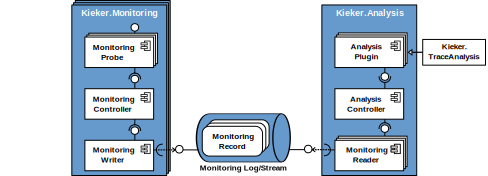
\includegraphics[width=0.96\textwidth]{images/kiekerComponentDiagram-woCloud-bw-w-record-newNames-withTraceAnalysis-colors}
\caption{Overview of the framework components}
\label{fig:KiekerComponentDiagram}
\end{figure}

\noindent The \KiekerMonitoringPart{} component is responsible for program instrumentation, data collection, and logging. Its core is the \class{MonitoringController}. %  which %
%receives the monitoring data in so-called monitoring records from monitoring probes, and writes these %
% receives the monitoring data and passes it to the configured monitoring log writer. %
%
The component \KiekerAnalysisPart{} is responsible for reading, analyzing, and visualizing the monitoring data. Its core is the \class{AnalysisController} which manages the life-cycle of the pipe-and-filter architecture of analysis plugins, including monitoring readers and  analysis filters.

The monitoring and analysis parts of the \Kieker{} framework are composed of subcomponents which represent the different functionalities of the monitoring and analysis tasks. The important interaction pattern among the components is illustrated in Figure~\ref{fig:KiekerCommunicationDiagram} but will be explained furthermore throughout the course of this user guide.

\vspace{1cm}

% This image shows the communication diagram of the different components.
\begin{figure}[H]\centering
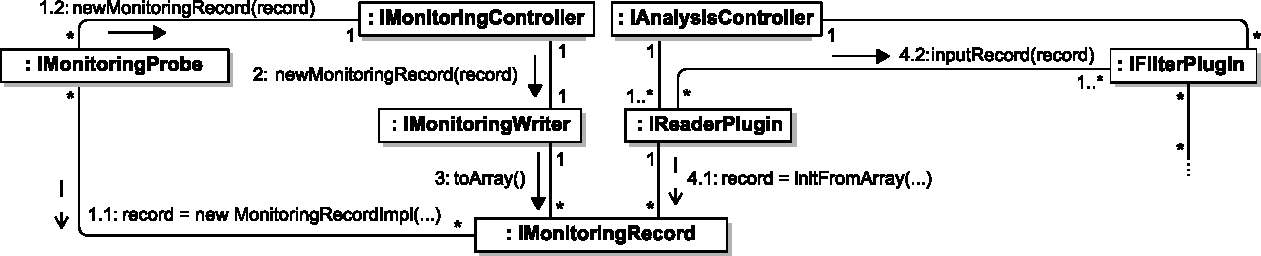
\includegraphics[width=1\textwidth]{images/kiekerCommunications-revisedReArranged-woMonitoringLog-bw-newNames}
\caption{Communication among \Kieker{} framework components}
\label{fig:KiekerCommunicationDiagram}
\end{figure}

% \vspace{1cm}

% Notify-tag because it is explained how Kieker works.
% avh: removed
\noindent The monitoring probes create the monitoring records containing the %
monitoring data and deliver them to the monitoring controller. %
The monitoring controller employs the monitoring writers to write these %
monitoring records to a monitoring log or stream. %
For analyzing purposes, monitoring reader plugins read the records from the %
monitoring log/stream. These records can then be further processed by a %
configuration of additional filter and repository plugins, inter-connected via input and output ports. %

\section{Framework Components and Extension Points}

\begin{figure}\centering
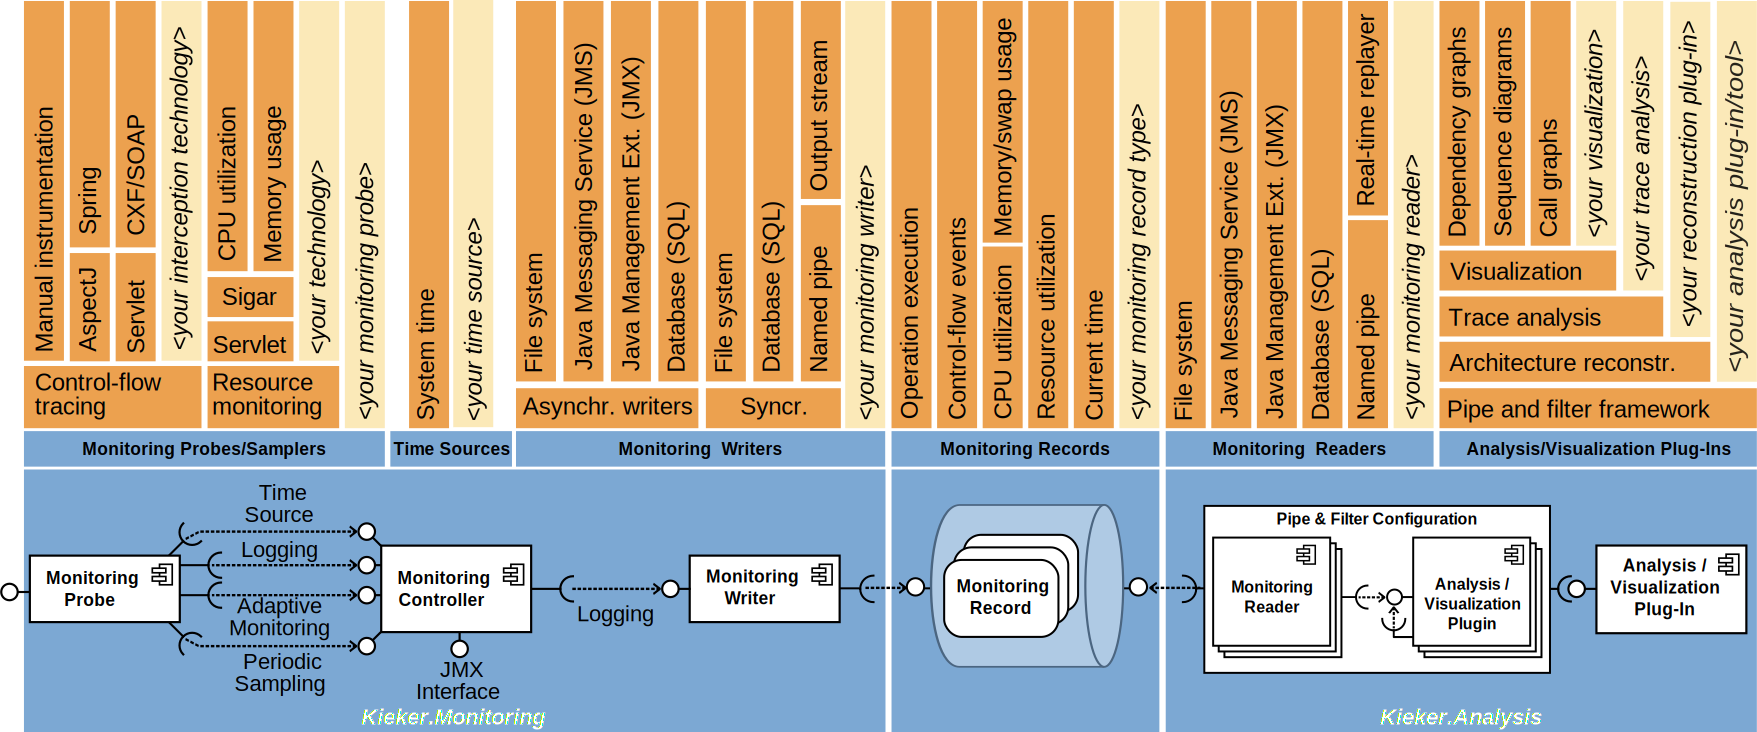
\includegraphics[width=\textwidth]{images/framework-figure}
\caption{Kieker framework components and extension points for custom components}
\label{fig:frameworkComponentsExtensionPoints}
\end{figure}

Figure~\ref{fig:frameworkComponentsExtensionPoints} depicts the possible %
extension points for custom components as well as the components which %
are already included in the \Kieker{} distribution and detailed below. %

\medskip

\begin{compactitem}
 \item \textbf{Monitoring writers and corresponding readers} for %
file systems and SQL databases, %
for in-memory record streams (named pipes), %
as well writers and readers employing Java Management %
Extensions (JMX)~\cite{JMX-Website} and %
Java Messaging Service~(JMS)~\cite{JMS-WebSite} technology. %
A special reader allows to replay existing persistent %
monitoring logs, for example to emulate incoming monitoring %
data---also in real-time.
 \item \textbf{Time sources} utilizing Java's \method{System.nanoTime()} (default) %
or \method{System.current\-TimeMillis()} methods.
 \item \textbf{Monitoring record types} allowing to store %
monitoring data about operation executions (including timing, control-flow, %
and session information), CPU and resource utilization, memory/swap usage, as well as %
a record type which can be used to store the current time.
\item \textbf{Monitoring probes}: A special feature of \Kieker{} is the ability to monitor (distributed) %
traces of method executions and corresponding timing information. %
For monitoring this data, Kieker includes monitoring probes employing %
AspectJ~\cite{AspectJ-WebSite}, %
Java~EE Servlet~\cite{JavaServletTechnology-WebSite}, %
Spring~\cite{Spring-WebSite}, and %
Apache~CXF~\cite{CXF-WebSite} technology. %
Additionally, Kieker includes probes for (periodic) system-level resource %
monitoring employing the Sigar library~\cite{HypericSigarWebsite}.
\item \textbf{Analysis/Visualization plugins} can be assembled to %
pipe-and-filter architectures based on input and output ports. The %
\KiekerTraceAnalysis{} tool 
% (Figure~\ref{fig:KiekerComponentDiagram}) %
% nie: Removed as this seems to be a wrong figure for this tool
is itself implemented based on a re-usable set of \KiekerAnalysisPart{} %
plugins allowing to reconstruct and visualize architectural models of the %
monitored systems, e.g., as dependency graphs, sequence diagrams, and call %
trees. %
\end{compactitem}



%%
% \pagebreak

\section{Licensing}

\Kieker{} is licensed under the Apache License, Version 2.0. You may obtain a copy of %
the license at \url{http://www.apache.org/licenses/LICENSE-2.0}.

The \Kieker{} source and binary release archives include a number of third-party %
libraries. %
% Appendix~\ref{appendix:libraries} lists these libraries along with information %
% on the licenses. 
The \dir{lib/} directory of the release archives contains a %
\file{.LICENSE} file for each third-party library, pointing to the respective license text.

\section{Citing Kieker}\label{sec:ch1:citingKieker}

When referencing Kieker resources in your publications, we would be happy if you %
respected the following guidelines:

\begin{itemize}
\item When referencing the Kieker project, please cite our %
ICPE~2012~\cite{KiekerICPE2012} paper and/or our 2009 technical report~\cite{vanHoornRohrHasselbringWallerEhlersFreyKieselhorst2009TRContinuousMonitoringOfSoftwareServicesDesignAndApplicationOfTheKiekerFramework}. %
Also, you might want to add a reference to our web site (\url{http://kieker-monitoring.net/}) %
like~\cite{KiekerWebSite}. 
\item When referencing this user guide, e.g., when reprinting contents, please %
use a citation like~\cite{KiekerUserGuideThis}.
\end{itemize}

\noindent At \url{http://kieker-monitoring.net/research/publications/} we provide %
entries for $\mathrm{B\scriptstyle IB}\!$\TeX{} and other bibliography %
systems.

\section{Kieker is Recommended by the SPEC Research Group}

In 2011, Kieker was reviewed and accepted for distribution as part of the SPEC Research %
Group's repository of peer-reviewed tools for quantitative system evaluation and analysis. %
See \url{http://research.spec.org/projects/tools.html} for details.

\section{Structure of this User Guide}

Based on a simple example, Chapter~\ref{chap:example} demonstrates %
how to manually instrument Java programs with \KiekerMonitoringPart{} %
in order to monitor timing information of method executions, and %
how to use \KiekerAnalysisPart{} to analyze the monitored data. %
Chapter~\ref{chap:componentsMonitoring} provides a more detailed %
description of \KiekerMonitoringPart{} and shows how to implement and %
use custom monitoring records, monitoring probes, and monitoring writers. %
A more detailed description of \KiekerAnalysisPart{} and how to implement and use %
custom monitoring readers, and analysis plugins follows in %
Chapter~\ref{chap:componentsAnalysis}. %
Chapter~\ref{chap:aspectJ} demonstrates how to use \KiekerTraceAnalysis{} %
for monitoring, analyzing, and visualizing trace information. %
Additional resources are included in the \hyperlink{hypertarget:appendix}{Appendix}, %
e.g., analyzing Java\,EE systems, using the JMS writers and readers, %
as well as monitoring system-level measures (CPU, memory, etc.) with %
Sigar. %

\vspace{1cm}

% Notify-tag because this could be interesting for the reader.
\NOTIFYBOX{The Java sources presented in this user guide, as well as pre-compiled binaries, %
are included in the %
\file{\exampleReleaseDir/} directory of the \Kieker{} distribution (see %
Section~\ref{sec:example:downloadInstall}). Also, the example directories can %
be imported as Eclipse projects.}


% \TODO{Point to Web site for additional examples, TR, \ldots}

  %%%%%%%%%%%%%%%%%%%%%%%%%%%%%%%%%%%%%%%%%
% Quick Start Example
%
% $Date$
% $Rev$:
% $Author$


\chapter{Quick Start Example}\label{chap:example}

This chapter provides a brief introduction to \Kieker{} based on a simple Bookstore example application. Section~\ref{sec:example:downloadInstall} explains how to download and install \Kieker{}. The Bookstore application itself is introduced in Section~\ref{sec:example:bookstore}, while the following sections demonstrate how to use \Kieker{} for monitoring~(Section~\ref{sec:example:monitoring}) and analyzing~(Section~\ref{sec:example:analysis}) the resulting monitoring data.

%%
\section{Download and Installation}\label{sec:example:downloadInstall}

The \Kieker{} download site\footnote{\KiekerDownloadURL{}} provides archives of the binary and source distribution, the Javadoc~API, as well as additional examples. For this quick start guide, \Kieker{}'s binary distribution, e.g., \file{\binaryFileForDownload}, is required and must be downloaded. After having extracted the archive, you'll find the directory structure and contents shown in Figure~\ref{fig:binary-layout}.

\enlargethispage{0.8cm}

% Note: The indention is not really necessary, but the tree is easier to understand in the tex-source.
\begin{figure}[h!]%[H]
\begin{graybox}
\dirtree{%
  .1 \DirInDirTree{\KiekerDir/}.
    .2 \DirInDirTree{bin/}\DTcomment{Call scripts for \Kieker{} tools}.
      .3 \ldots.
    .2 \DirInDirTree{build/libs/}\DTcomment{The \Kieker{} framework libraries}.
      .3 \mainJar.
      .3 \ldots. %\servletWar.
    .2 \DirInDirTree{doc/}\DTcomment{}.
      .3 kieker-\version\_userguide.pdf\DTcomment{PDF file of this document}.
    .2 \DirInDirTree{examples/}\DTcomment{Example projects and configuration files}.
      .3 \DirInDirTree{userguide/}\DTcomment{Source code of the examples in this document}.
                        .4 \ldots.
      .3 \kiekerExampleMonitoringProperties{}.
    .2 \DirInDirTree{lib/}\DTcomment{Libraries required by \Kieker{}}.
%       .3 \commonsLoggingJar.
      .3 \ldots.
}
\end{graybox}
\caption{Directory structure and contents of \Kieker{}'s binary distribution}
\label{fig:binary-layout}
\end{figure}

\pagebreak

The Java sources presented in this user guide, as well as pre-compiled binaries, are included in the \file{\exampleReleaseDir/} directory. The file \file{\mainJar{}} contains the \KiekerMonitoringPart{} and \KiekerAnalysisPart{} components, as well as the \KiekerTraceAnalysis{} tool. The sample \KiekerMonitoringPart{}
configuration file %
\file{\kiekerExampleMonitoringProperties{}} will be detailed in Chapter~\ref{chap:componentsMonitoring}. %
In addition to the \file{\mainJar{}} file, the \file{build/libs/} directory includes %
variants of this \file{.jar} files with integrated third-party libraries. Additional %
information on these \file{.jar} files and when to use them will follow later in this document. %

% Since \Kieker{} uses the Apache Commons library~\cite{CommonsLogging-WebSite} as a logging interface, the file \file{\commonsLoggingJar} is the only dependency to a third-party library which is needed to execute \Kieker{} in any case.

%%
\section{Bookstore Example Application}\label{sec:example:bookstore}

The Bookstore application is a small sample application resembling a simple bookstore with a market-place facility where users can search for books in an online catalog, and subsequently get offers from different book sellers.
Figure~\ref{fig:bookstore:classAndSequenceDiagrams} shows a class diagram describing the structure of the bookstore and a sequence diagram illustrating the dynamics of the application.

\begin{figure}[h]\centering
\subfigure[]{\label{fig:boostore:classdiagram}%
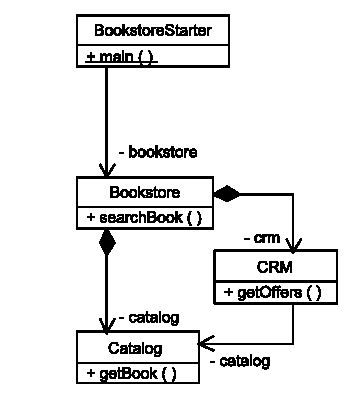
\includegraphics[scale=0.83]{images/kieker_bookstoreclassdiagram}%
}%
\subfigure[]{\label{fig:boostore:sequencediagram}%
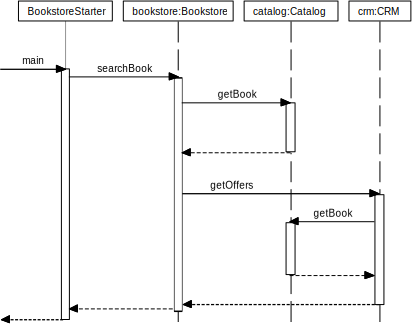
\includegraphics[scale=0.83]{images/kieker_SequenceDiagram-manually-changed}%
}
\caption{UML class diagram~\subref{fig:boostore:classdiagram} and sequence diagram~\subref{fig:boostore:sequencediagram} of the Bookstore application}
\label{fig:bookstore:classAndSequenceDiagrams}
\end{figure}

\pagebreak

The bookstore contains a catalog for books and a customer relationship management system~(CRM) for the book sellers. To provide this service, the different classes provide operations to initialize the application, search for books, and get offers or searched books. In this example, the methods implementing these operations are merely stubs. However, for the illustration of \Kieker{} they are sufficient and the inclined reader may extend the application into a real bookstore.

The directory structure of the Bookstore example is shown in Figure~\ref{fig:PlainBookstoreExample} and comprises four Java classes in its source directory \dir{src/.../ch2bookstore/}, which are explained in detail below.

\begin{figure}[H]
\begin{graybox}
\dirtree{%
.1 \DirInDirTree{examples/}. %\DTcomment{The root directory of the project}.
.2 \DirInDirTree{userguide/}.
.3 \DirInDirTree{ch2--bookstore-application/}.
.4 \DirInDirTree{src/}\DTcomment{The directory for the source code files}.
.5 \DirInDirTree{.../ch2bookstore/}.
.6 Bookstore.java.
.6 BookstoreStarter.java.
.6 Catalog.java.
.6 CRM.java.
.5 build.gradle\DTcomment{Optional build script for the application}.
.5 gradlew.
.5 gradlew.bat.
.5 README.txt.
}
\end{graybox}

\caption{The directory structure of the Bookstore application}
\label{fig:PlainBookstoreExample}
\end{figure}

\NOTIFYBOX{The Java sources and a pre-compiled binary of the uninstrumented Bookstore application can be found in the \file{\plainBookstoreApplicationReleaseDirDistro{}/} directory.}

\quad\

\enlargethispage{1cm}

\noindent The class \class{BookstoreStarter} contains the application's \method{main} method (shown in Listing~\ref{lst:class:BookstoreStarter}), i.e., the program start routine. It initializes the \class{Bookstore} and issues five search requests by calling the \method{searchBook} method of the \object{bookstore} object.

\medskip

\setJavaCodeListing
\lstinputlisting[caption=\method{main} method from BookstoreStarter.java,firstline=23,firstnumber=23,lastline=29,label=lst:class:BookstoreStarter]{\plainBookstoreApplicationDir/src/kieker/examples/userguide/ch2bookstore/BookstoreStarter.java}

\pagebreak

\noindent The \class{Bookstore}, shown in Listing~\ref{lst:class:Bookstore}, contains a catalog and a CRM object, representing the catalog of the bookstore and a customer relationship management system which can provide offers for books out of the catalog. The business method of the bookstore is \method{searchBook()} which will first check the catalog for books and then check for offers.

In a real application these methods would pass objects to ensure the results of the catalog search will be available to the offer collecting method. However, for our example we omitted such code.

\lstinputlisting[caption=Bookstore.java,label=lst:class:Bookstore,firstline=19,firstnumber=19]{\plainBookstoreApplicationDir/src/kieker/examples/userguide/ch2bookstore/Bookstore.java}

\noindent The customer relationship management for this application is modeled in the \class{CRM} class shown in Listing~\ref{lst:class:CRM}. It provides only a business method to collect offers by using the catalog for some lookup. The additional catalog lookup is later used to illustrate different traces in the application.

\lstinputlisting[caption=CRM.java,label=lst:class:CRM,firstline=19,firstnumber=19]{\plainBookstoreApplicationDir/src/kieker/examples/userguide/ch2bookstore/CRM.java}

% \pagebreak

\enlargethispage{0.8cm}

\noindent Finally, the class \class{Catalog} is shown in Listing~\ref{lst:class:Catalog}. It resembles the catalog component in the application.

\lstinputlisting[caption=Catalog.java,label=lst:class:Catalog,firstline=19,firstnumber=19]{\plainBookstoreApplicationDir/src/kieker/examples/userguide/ch2bookstore/Catalog.java}

\noindent After this brief introduction of the application and its implementation, the next step is to see the example running. To compile and run the example, the commands in Listing~\ref{lst:bookstoreStarterNoInstr} can be executed. This document assumes that the reader enters the commands in the example directory. For this first example this is \dir{examples/userquide/ch2--bookstore-application/}.
\\
\NOTIFYBOX{Windows comes with two command-line interpreters called \texttt{cmd.exe} and \texttt{command.com}. Only the first one is able to handle wildcards correctly. So we recommend using \texttt{cmd.exe} for these examples.}

\setBashListing
% \input{ch2-quickstart-example_Compile_Run_Example_1-noinstr.inc}
% \WARNBOX{The default command-line interpreter of Windows doesn't support automatic file expansion. Therefore every single sourcefile has to be passed:
%\input{ch2-quickstart-example_Compile_Run_Example_1-noinstr-win.inc}%
%}
\begin{lstlisting}[label=lst:bookstoreStarterNoInstr, caption=Commands to compile and run the Bookstore application]
> mkdir build
> javac src/kieker/examples/userguide/ch2bookstore/*.java -d build

> java -classpath build kieker.examples.userguide.ch2bookstore.BookstoreStarter
\end{lstlisting}

\noindent The first command compiles the application and places the resulting four class files in the \dir{build/} directory. To verify the build process, the \dir{build/} directory can be inspected. The second command loads the bookstore application and produces the output shown in Listing~\ref{lst:result-noinstr}.

\begin{lstlisting}[caption=Example run of the Bookstore application,label=lst:result-noinstr]
Bookstore.main: Starting request 0
Bookstore.main: Starting request 1
Bookstore.main: Starting request 2
Bookstore.main: Starting request 3
Bookstore.main: Starting request 4
\end{lstlisting}


\noindent In this section, the \Kieker{} example application was introduced and when everything went well, the bookstore is a runnable program. Furthermore, the composition of the application and its function should now be present. %
The next Section~\ref{sec:example:monitoring} will demonstrate how %
to monitor this example application employing \KiekerMonitoringPart{} using manual instrumentation.

\pagebreak

%%
\section{Monitoring with \KiekerMonitoringPart{}}\label{sec:example:monitoring}

In the previous Sections~\ref{sec:example:downloadInstall} and \ref{sec:example:bookstore}, the \Kieker{} installation and the example application have been introduced. In this section, the preparations for application monitoring, the instrumentation of the application, and the actual monitoring are explained.

\quad\

\WARNBOX{In this example, the instrumentation is done manually. %
This means that the monitoring probe is implemented by mixing monitoring logic %
with business logic, which is often not desired since the resulting code is %
hardly maintainable. \Kieker{} includes probes %
based on AOP (aspect-oriented programming, \cite{Kiczales1997}) %
technology, as covered by Chapter~\ref{chap:aspectJ}. However, to illustrate the %
instrumentation in detail, the quick start example uses manual instrumentation.}

\

\noindent The first step is to copy the \Kieker{} jar-file \file{\mainJarEMF} to the \dir{lib/} directory of the example directory~(see Section~\ref{sec:example:bookstore}). The file is located in the \dir{\KiekerDir/build/libs/} directory of the extracted \Kieker{} archive, as described in Section~\ref{sec:example:downloadInstall}. %
In the example directory for this section, this file is already included, %
as illustrated in Figure~\ref{fig:KiekerBookstoreExample}.

\begin{figure}[H]
\begin{graybox}
\dirtree{%
.1 \DirInDirTree{examples/}. %\DTcomment{The root directory of the project}.
.2 \DirInDirTree{userguide/}.
.3 \DirInDirTree{ch2--manual-instrumentation/}.
.4 \DirInDirTree{build/}\DTcomment{Directory for the Java class files}.
.4 \newFileDirInDirTree{\DirInDirTree{lib/}}\DTcomment{Directory for the required libraries}.
.5 \newFileDirInDirTree{\mainJarEMF}.
.4 \DirInDirTree{src/}\DTcomment{The directory for the source code files}.
.5 \ldots.
}
\end{graybox}
\caption{The directory structure of the Bookstore application with \Kieker{} libraries}
\label{fig:KiekerBookstoreExample}
\end{figure}

\NOTIFYBOX{The Java sources and pre-compiled binaries of the manually instrumented Bookstore application described in %
this section can be found in the \file{\manualInstrumentedBookstoreApplicationReleaseDirDistro{}/} directory.}

\quad\

\noindent \Kieker{} maintains monitoring data as  so-called monitoring records. %
Section~\ref{sec:componentsMonitoring:monitoringRecords} describes how to define and use custom monitoring record types. %
The monitoring record type used in this example is an \textit{operation execution record} which %
is included in the \Kieker{} distribution. %
Figure~\ref{fig:OperationExecutionRecordClassDiagram} shows the %
attributes which  are relevant to this example. %
The record type will be detailed in Chapter~\ref{chap:aspectJ} .

\begin{figure}[H]
\begin{centering}
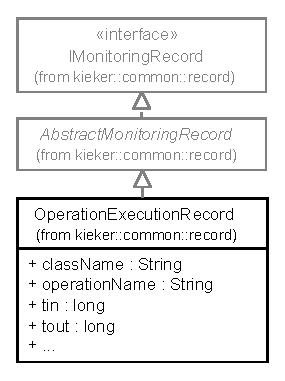
\includegraphics[scale=1]{images/kieker_OperationExecutionRecord-notraceattributes-inheritance}%
\caption{The class diagram of the operation execution record}
\label{fig:OperationExecutionRecordClassDiagram}
\end{centering}
\end{figure}

\noindent The attributes relevant to this part are \method{operationSignature} and \method{hostname}, %
as well as \method{tin} and \method{tout} for %
the timestamps before and after the call of the instrumented method.

\enlargethispage{1.2cm}

Listing~\ref{lst:cuttingBookstore} shows the instrumentation of the \class{Bookstore} class and its method \method{searchBook()}. In the lines~25 and~26, the monitoring controller is instantiated. It provides the monitoring service for the instrumentation.

% \TODO{Imports?!\\ --- avh: ja, evtl. mit linerange, aber er bl\"oderweise nummeriert er so durch}
% Make sure that this listing will be modified, once the sourcecode changes!!!
% It must show the whole monitoring of the bookstorecall, from getting the first time to persisting of the record!!

\setJavaCodeListing
\lstinputlisting[linerange={25-49}, firstnumber=25, caption=Instrumentation of the \method{getBook()} call in Bookstore.java, label=lst:cuttingBookstore]%
{\manualInstrumentedBookstoreApplicationDir/src/kieker/examples/userguide/ch2bookstore/manual/Bookstore.java}

\noindent The lines~32 and~34 are used to determine the current time in nanoseconds before and after the \method{getBook()} call. In lines~36 to~42, a monitoring record for this measurement is created and initialized, passing the method signature, the hostname, and the two time values as arguments. Finally the record is handed over to the monitoring controller (line~43) which calls a monitoring writer to persist the record. %
In this example, the filesystem writer is used---\Kieker{} uses this writer by default when no other writer is specified, %
as detailed in Section~\ref{sec:monitoring-log-writers}. %.

In addition to the instrumentation in the \class{Bookstore} class, the \method{getOffers()} method of the \class{CRM} class is instrumented as well. Similar to Listing~\ref{lst:cuttingBookstore}, measurements are taken before and after the call of the \object{catalog}'s \method{getBook()} method, as shown in %
lines~36 and~38 of Listing~\ref{lst:cuttingCRM}. Not shown in the listing is the instantiation of the monitoring controller. However, it is done in the same way as illustrated in Listing~\ref{lst:cuttingBookstore}. %And the complete example files can be found in the samples directory.
Finally, a record is created (see lines~40--46) and stored by calling the monitoring controller (see line~47).

\setJavaCodeListing
\lstinputlisting[firstline=34, firstnumber=34, lastline=48, caption=Instrumentation of the \method{getBook()} call in CRM.java, label=lst:cuttingCRM]%
{\manualInstrumentedBookstoreApplicationDir/src/kieker/examples/userguide/ch2bookstore/manual/CRM.java}

% \enlargethispage{0.5cm}

\noindent %
The next step after instrumenting the code is running the instrumented application. Listing~\ref{lst:bookstoreStarterLinux} shows the commands to compile and run the application under \UnixLikeSystems{}. Listing \ref{lst:bookstoreStarterWin} shows the same commands for Windows. The expected working directory is the base directory of this example, i.e. %
 \dir{\manualInstrumentedBookstoreApplicationReleaseDirDistro{}/}.
 
% \pagebreak

\enlargethispage{1cm}

\setBashListing
\begin{lstlisting}[caption=Commands to compile and run the instrumented Bookstore under \UnixLikeSystems{},label=lst:bookstoreStarterLinux]
#\lstshellprompt{}# javac src/kieker/examples/userguide/ch2bookstore/manual/*.java 
       -classpath lib/#\mainJarEMF# -d build/

#\lstshellprompt{}# java -classpath build/:lib/#\mainJarEMF#
       kieker.examples.userguide.ch2bookstore.manual.BookstoreStarter
\end{lstlisting} 

% \quad\

\WARNBOX{%
Under Windows it is necessary to separate the classpath elements by %
a semicolon instead of a colon. Also, we recommend to use the Windows shell %
\file{cmd.exe} for this tutorial since problems have been reported for the %
Windows PowerShell.}

% \pagebreak

\begin{lstlisting}[caption=Commands to compile and run the instrumented Bookstore under Windows,label=lst:bookstoreStarterWin]
#\lstshellprompt{}# javac src\kieker\examples\userguide\ch2bookstore\manual\*.java  
       -classpath lib\#\mainJarEMF# -d build\

#\lstshellprompt{}# java -classpath build\;lib\#\mainJarEMF#
       kieker.examples.userguide.ch2bookstore.manual.BookstoreStarter
\end{lstlisting}

\quad\

\noindent If everything worked correctly, a new directory for the monitoring data with a name similar to \dir{kieker-20120402-163314855-UTC-myHost-KIEKER-SINGLETON/} is created % in the default temporary directory
(see Figure~\ref{fig:logtree}). %
% The numbers in the directory name represent the time and date of the monitoring. %Thus, they will be different numbers for every run.
In \Kieker's default configuration, the log directory can be found in the default temporary directory: %
under \UnixLikeSystems{}, this is typically \dir{/tmp/}; %
check the environment variables \dir{\$TMPDIR} or \dir{\%temp\%} for the location under Mac OS or Windows respectively. %
The exact location of the created monitoring log is reported in \Kieker's console output (see for example Appendix~\ref{sec:appendix:manualInstrumentation:output}).
%it \dir{C:\textbackslash{}users\textbackslash{}[\ldots]\textbackslash{}temp} under Windows.
The monitoring directory contains two types of files: \dir{.dat} files containing text representations of the monitoring records and a %single
file named \dir{kieker.map} which contains information on the types of monitoring records used.

\begin{figure}[H]
\begin{graybox}
\dirtree{%
.1 \DirInDirTree{/tmp/}.
.2 \DirInDirTree{kieker-20130910-120352847-UTC-myHost-KIEKER-SINGLETON/}.
.3 kieker.map.
.3 kieker-20120402-163314882-UTC--000-Thread-1.dat.
}
\end{graybox}
\caption{Directory structure after a monitoring run}
\label{fig:logtree}
\end{figure}

\enlargethispage{1cm}

The Listings~\ref{lst:exampledat} and \ref{lst:examplemap} show example file contents. The \file{.dat}-file is saved in CSV format (\textbf{C}omma \textbf{S}eparated \textbf{V}alues)---in this case, the values of a monitoring record are separated by semicolons. To understand the \file{.dat}-file structure the semantics have to be explained. For this quick start example only some of the values are relevant. The first value \verb!$1! indicates the record type. The fourth value indicates the class and method which has been called. And the seventh and eighth value are the start and end time of the execution of the called method.

\setBashListing
\lstinputlisting[caption=kieker-20130910-120352862-UTC-000-Thread-1.dat (excerpt), firstline=1, lastline=2, label=lst:exampledat]%
{ch2-quickstart-example/kieker-20130910-120352847-UTC-myHost-KIEKER-SINGLETON/kieker-20130910-120352862-UTC-000-Thread-1.dat}

\noindent The second file is a simple mapping file referencing keys to monitoring record types. In Listing~\ref{lst:examplemap} the key \verb!$1! is mapped to the type of operation execution records which were used in the monitoring. The key value corresponds to the key values in the \file{.dat}-file.

\lstinputlisting[caption=kieker.map, label=lst:examplemap]%
{ch2-quickstart-example/kieker-20130910-120352847-UTC-myHost-KIEKER-SINGLETON/kieker.map}

\noindent By the end of this section, two Java classes of the Bookstore application %
have been manually instrumented using \KiekerMonitoringPart{} and at least one %
run of the instrumented application has been performed. %
The resulting monitoring log, written to the \file{.dat}-file in CSV format, could %
already be used for analysis or visualization by any spreadsheet or %
statistical tool. %
The following Section~\ref{sec:example:analysis} will show how to process %
this monitoring data with \KiekerAnalysisPart{}.

%%
\section{Analysis with \KiekerAnalysisPart{}}\label{sec:example:analysis}

%The last task of a successful application monitoring is the analysis of the collected information.
In this section, the monitoring data recorded in the previous section is %
analyzed with \KiekerAnalysisPart{}. %
% The second step is to write a suitable analyzer. And finally the analyzer is used to aggregate the information in a sensible way.
For this quick example guide, the analysis tool is very simple and does not show %
the full potential of \Kieker{}. For more detail, read %
Chapter~\ref{chap:componentsAnalysis} to learn which plugins, i.e., readers %
and filters, are included in \Kieker{}, how to use them, and how to develop %
custom plugins. %
Chapter~\ref{chap:aspectJ} presents the \KiekerTraceAnalysis{} tool, which %
is also based on \KiekerAnalysisPart{}.
\KiekerAnalysisPart{} has a dependency to the Eclipse Modeling Framework~(EMF).%
\footnote{\url{http://www.eclipse.org/modeling/emf/}} %
For this reason, we are using the \file{\mainJarEMF{}} that is a variant of %
the \file{\mainJar{}}, additionally including the required EMF dependencies. %
When using the \file{\mainJar{}}, the \file{org.eclipse.emf.\-*.jar} files (to %
be found in \Kieker's \file{lib/} directory) need to be added to the classpath. %

\begin{figure}[H]
\begin{graybox}
\dirtree{%
.1 \DirInDirTree{examples/}. %\DTcomment{The root directory of the project}.
.2 \DirInDirTree{userguide/}.
.3 \DirInDirTree{ch2--manual-instrumentation/}.
.4 \DirInDirTree{build/}\DTcomment{Directory for the Java class files}.
.4 \newFileDirInDirTree{\DirInDirTree{lib/}}\DTcomment{Directory for the required libraries}.
.5 \newFileDirInDirTree{\mainJarEMF}.
.4 \DirInDirTree{src/}\DTcomment{The directory for the source code files}.
.5 \DirInDirTree{.../manual/}.
.6 \ldots.
.6 \newFileDirInDirTree{BookstoreAnalysisStarter.java}.
}
\end{graybox}
\caption{Directory layout of the example application with the analysis files highlighted}
\label{lst:analysisExampleLayout}
\end{figure}

\noindent The analysis application developed in this section comprises the file %
\file{BookstoreAnalysisStarter.java}, as shown in Figure~\ref{lst:analysisExampleLayout}. %
This file can also be found in the directory \dir{\manualInstrumentedBookstoreApplicationReleaseDirDistro{}/}.
The file sets up the basic pipe-and-filter configuration depicted in Figure~\ref{fig:example:ch2:pipe-and-filter}: %
\Kieker{}'s file system reader (\class{FSReader}) reads monitoring records %
from a file system monitoring log (as produced in the previous Section~\ref{sec:example:monitoring}) %
and passes these to the \class{TeeFilter} plugin; the \class{TeeFilter} plugin %
reads events of arbitrary type (i.e., Java \class{Object}), prints them to a %
configured output stream, and also relays them to filters connected to the %
filter's output port \method{relayedEvents}. %

\begin{figure}[h]
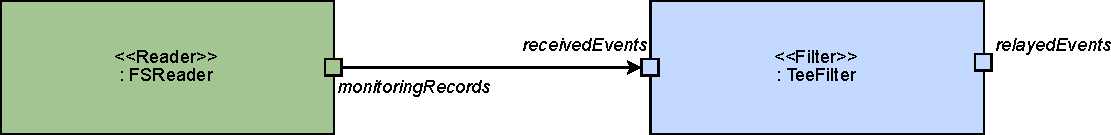
\includegraphics[width=\textwidth]{images/ch2-example-pnp}
\caption{Example pipe-and-filter configuration}
\label{fig:example:ch2:pipe-and-filter}
\end{figure}

\enlargethispage{0.5cm}

\KiekerAnalysisPart{} pipe-and-filter configurations can %
be created programmatically, i.e., by configuring, instantiating, and %
connecting the plugins in a Java program.%
\footnote{As an alternative, a web-based user interface is available for \Kieker{} \cite{KiekerWebSite}} %
For the example, this is demonstrated in Listing~\ref{lst:BookstoreAnalysisStarter}, %
which shows an excerpt from the \class{BookstoreAnalysisStarter}'s \method{main} %
method. %

% \pagebreak

\setJavaCodeListing
\lstinputlisting[gobble=4,caption=BookstoreAnalysisStarter.java (excerpt from \method{main} method),label=lst:BookstoreAnalysisStarter,firstline=37,firstnumber=37,lastline=56]%
{\manualInstrumentedBookstoreApplicationDir/src/kieker/examples/userguide/ch2bookstore/manual/BookstoreAnalysisStarter.java}

% \pagebreak

\noindent The \class{BookstoreAnalysisStarter} follows a simple scheme. Each %
analysis tool has to create at least one \class{AnalysisController} which can be %
seen in Listing~\ref{lst:BookstoreAnalysisStarter} in line~38. Then, the plugins, %
which may be readers or filters, are configured, and instantiated. The usage of the  %
constructor ensures that the component is registered with the analysis instance. %
Lines~41--43 configure, instantiate, and register the file system monitoring %
log reader, which uses the command-line argument value as the input directory. %
The application expects the %
output directory from the earlier monitoring run (see Section~\ref{sec:example:monitoring}) %
as the only argument value, which must be passed manually. %
Lines~46--49 configure, instantiate, and register the \class{TeeFilter}, %
which outputs received events to the standard output. Lines~52 and~53 connect %
the \class{TeeFilter}'s input port to the filesystem reader's output port. %
The analysis is started by calling its \method{run} method (line~56). %


The Listings~\ref{lst:bookstoreAnalysisStarterLinux} and \ref{lst:bookstoreAnalysisStarterWin} %
describe how the analysis application can be compiled and executed under \UnixLikeSystems{} and Windows.

\setBashListing
\enlargethispage{1.0cm}
\begin{lstlisting}[caption=Commands to compile and run the analysis under \UnixLikeSystems{},label=lst:bookstoreAnalysisStarterLinux] 			
#\lstshellprompt{}# javac src/kieker/examples/userguide/ch2bookstore/manual/*.java 
        -classpath lib/#\mainJarEMF# -d build/

#\lstshellprompt{}# java -classpath build/:lib/#\mainJarEMF#
       kieker.examples.userguide.ch2bookstore.manual.BookstoreAnalysisStarter 
       /tmp/kieker-20130910-120352847-UTC-myHost-KIEKER-SINGLETON
\end{lstlisting}	

\begin{lstlisting}[caption=Commands to compile and run the analysis under Windows,label=lst:bookstoreAnalysisStarterWin]
#\lstshellprompt{}# javac src\kieker\examples\userguide\ch2bookstore\manual\*.java 
        -classpath lib\#\mainJarEMF# -d build\

#\lstshellprompt{}# java -classpath build\;lib\#\mainJarEMF#
       kieker.examples.userguide.ch2bookstore.manual.BookstoreAnalysisStarter 
       C:\Temp\kieker-20130910-120352847-UTC-myHost-KIEKER-SINGLETON
\end{lstlisting}	



\noindent You need to make sure that the application gets the correct path from the monitoring run.
The \class{TeeFilter} prints an output message for each record received. %
An example output can be found in Appendix~\ref{sec:appendix:manualInstrumentation:output}.
% A possible display of the run can be found in the appendix of this tutorial.

  %%%%%%%%%%%%%%%%%%%%%%%%%%%%%%%%%%%%%%%%%
% Kieker Monitoring Component
%
% $Date$
% $Rev$:
% $Author$


\chapter{\KiekerMonitoringPart{} Component}\label{chap:componentsMonitoring}

% TODO (proposed by chw) separate between pure application and customization of Kieker.Monitoring
% TODO (proposed by chw) focus on common user scenarios, not on technical descriptions
% first: application
% - start with command line command/Eclipse
% - activate aspect/interceptor/... and configure it (e.g., pointcut in aop.xml)
% - configure Kieker.Monitoring
%   - include an excerpt of the properties file
%   - reference to the chapter of the writers
% second: customization
% - define a record
%   - with the IRL
%   - with Java by hand
% - define an aspect/interceptor/...
%   - mention here the role of the monitoring controller (currently chapter 3.1)

\NOTIFYBOX{The Java sources of this chapter, as well as a pre-compiled binary, %
can be found in the %
\file{\customComponentsBookstoreApplicationReleaseDirDistro{}/} directory of the %
binary release.}

\section{Monitoring Controller}\label{sec:componentsMonitoring:monitoringController}

The \class{MonitoringController} constructs and controls a \KiekerMonitoringPart{} %
instance.

\enlargethispage{1cm}

\begin{figure}[h]\centering % 
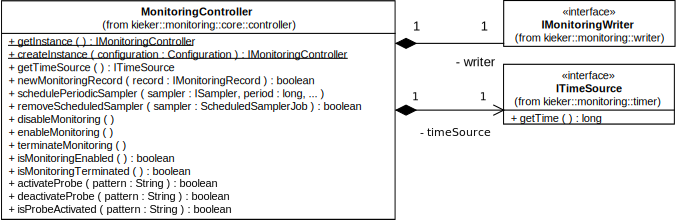
\includegraphics[scale=0.7]{images/kieker_monitoringControlleruserguide-simplified}
\caption{Class diagram of the \class{MonitoringController} (including selected methods)}
\label{fig:monitoringController:classdiagram}
\end{figure}

As depicted by the class diagram in Figure~\ref{fig:monitoringController:classdiagram}, it provides methods for\\

\begin{compactitem}
 \item Creating \class{IMonitoringController} instances (Section~\ref{sec:componentsMonitoring:monitoringController:factory}),
 \item Logging monitoring records with the configured monitoring writer (Section~\ref{sec:componentsMonitoring:monitoringController:logging}),
 \item Retrieving the current time via the configured time source (Section~\ref{sec:componentsMonitoring:monitoringController:getTime}),
 \item Scheduling and removing period samplers (Section~\ref{sec:componentsMonitoring:monitoringController:periodicSamplers}), 
 \item Controlling the monitoring state (Section~\ref{sec:componentsMonitoring:monitoringController:controState}), and
 \item Activating and deactivating probes at runtime \ref{sec:componentsMonitoring:monitoringController:adaptive}.
\end{compactitem}

\subsection{Creating \class{MonitoringController} Instances}\label{sec:componentsMonitoring:monitoringController:factory}

The \class{MonitoringController} provides two different static methods for retrieving instances of %
\class{IMonitoringController}:\\

\begin{compactenum}
 \item The method \method{MonitoringController.getInstance()} returns a singleton instance. %
As described in Section~\ref{sec:monitoring:configuration}, the configuration is read from %
a properties file that has been passed to the JVM, is located in the classpath, or %
conforms to the default configuration (Appendix~\ref{sec:appdx:monitoringproperties}). %
 \item The method \method{MonitoringController.createInstance(Configuration config)} can be utilized to create %
an instance that is configured according to the passed \class{Configuration} object, %
as described in Section~\ref{sec:monitoring:configuration}.
\end{compactenum}

\subsection{Logging Monitoring Records}\label{sec:componentsMonitoring:monitoringController:logging}

Monitoring records are sent to the configured monitoring writers by passing %
these records, in form of \class{IMonitoringRecord} objects, to the %
\class{MonitoringController}'s \method{newMonitoringRecord} method.  %
Note, that this is not the case if monitoring is disabled or terminated (Section~\ref{sec:componentsMonitoring:monitoringController:controState}).

\subsection{Retrieving the Current Time and Using Custom Time Sources}\label{sec:componentsMonitoring:monitoringController:getTime}

The current time is maintained by a so-called time source. The \class{MonitoringController}'s method %
\method{getTimeSource} returns an \class{ITimeSource} whose method %
\method{getTime} returns a timestamp in nanoseconds. \Kieker{}'s default %
time source, \class{SystemNanoTimer}, returns the current system %
time as the number of nanoseconds elapsed since 1 Jan 1970 00:00~UTC. %
The easiest way to use a custom time source is to extend the \class{AbstractTimeSource} and %
to implement the method \method{getTime()}. Custom time sources make sense, for example, %
in simulations where not the current system time but the current simulation time is %
relevant. The configuration needs to be adjusted to use a custom time source class. %

\subsection{Scheduling and Removing Periodic Samplers}\label{sec:componentsMonitoring:monitoringController:periodicSamplers}

For certain applications, it is required to monitor runtime data periodically, %
e.g., the utilization of system resources such as CPUs. %
For this purpose, \Kieker{} supports special monitoring probes, called samplers. %
Samplers must implement the interface \class{ISampler} which includes a %
single method \method{sample(IMonitoringController monitoringController)}. %
This method is called in periodic time steps, %
as specified by the \class{MonitoringController}'s registration function %
\method{schedulePeriodicSampler}. Periodic samplers can be stopped by %
calling the \class{MonitoringController}'s method \method{removeScheduledSampler}.

Listing~\ref{listing:sigarSamplerMethod} shows the \method{sample} method %
of the \class{MemSwapUsageSampler} which can be used to monitor memory %
and swap usage employing the Sigar library~\cite{HypericSigarWebsite}. %
Likewise to other monitoring probes described in this user guide (see for %
example Sections~\ref{sec:monitoring:probe} and \ref{sec:example:monitoring}),
it collects the data of interest (lines~61--62), creates a monitoring record~%
(lines~63--66), and passes this monitoring record to the monitoring controller~%
(line~67). %
The available Sigar-based samplers for monitoring system-level monitoring %
data, such as CPU and memory usage, are discussed in Appendix~\ref{appendix:SigarBasedSamplers}. %

\pagebreak

\setJavaCodeListing
\lstinputlisting[firstline=53, lastline=69, firstnumber=53, caption=Method \method{sample} from MemSwapUsageSampler.java, label=listing:sigarSamplerMethod]{../../kieker-monitoring/src/kieker/monitoring/sampler/sigar/samplers/MemSwapUsageSampler.java}

\subsection{Controlling the Monitoring State}\label{sec:componentsMonitoring:monitoringController:controState}

The \class{MonitoringController} provides methods to temporarily enable or disable monitoring %
(\method{enableMonitoring}/\method{disableMonitoring}), as well as to terminate monitoring %
permanently (\method{terminateMonitoring}). %
The current state can be requested by calling the methods \method{isMonitoringEnabled} %
and \method{isMonitoringTerminated}. If monitoring is not enabled (i.e., disabled %
or terminated), no monitoring records retrieved via the method \method{newMonitoringRecord} %
are passed to the monitoring writer. Also, probes should be passive or return immediately %
with respect to the return value of the method \method{isMonitoringEnabled}. %
Note, that once the \class{MonitoringController} is terminated, it cannot be enabled %
later on.

\subsection{Adaptive Monitoring}\label{sec:componentsMonitoring:monitoringController:adaptive}

The \class{MonitoringController} provides an API to activate and deactivate %
probes at runtime. By passing a method signature---e.g., %
\texttt{"public void Bookstore.getBook()"}---to the method %
\method{isProbeActivated}, probes can check whether or not monitoring for the %
method with the given signature is active. %
Monitoring can be (de)activated for single signature \textit{patterns}---e.g., %
\texttt{"public void Bookstore.*(..)"}--- via the methods %
\method{activateProbe} and \method{deactivateProbe}. The current list of %
(de)activated patterns can be obtained via the method \method{getProbePatternList}. %
The entire list can be replaced using the method \method{setProbePatternList}. %
Alternatively, a file with include and exclude patterns can be used. This file %
can be polled in regular intervals. %
A default configuration file, including a description of the pattern syntax, is provided %
by the file \file{kieker.monitoring.adaptiveMon\-i\-tor\-ing.example.conf} in the %
\dir{examples/} directory of the binary release. %

With the same mechanism arbitrary probes can be controlled. The syntax is also included %
in the above file. For example, \Kieker's probes for CPU and memory make use of %
this mechanism.

By default, \Kieker{}'s adaptive monitoring feature is deactivated. It can be %
enabled by setting the value of the configuration property %
\lstinline{kieker.monitoring.adaptiveMonitoring.enabled} %
in the \file{\monitoringPropertiesFile} file to \textit{true}. Additional properties %
to configure the adaptive monitoring are included in the file %
\file{kieker.monitoring.proper\-ties}, e.g., the location of the afore-mentioned file with %
include/exclude patterns and the polling interval for this file. 

\enlargethispage{0.8cm}

\subsection{JMX MBean Access to \class{MonitoringController}}

The \class{MonitoringController}'s %
interface methods (see Figure~\ref{fig:monitoringController:classdiagram}) can be accessed %
as a JMX MBean. For example, this allows to control the monitoring state using %
the methods described in the previous Section~\ref{sec:componentsMonitoring:monitoringController:controState}. %
As a JMX-compliant graphical client that is included in the JDK, \class{jconsole} %
is probably the easiest way to get started. Just keep in mind to add \Kieker{} to the classpath when calling \class{jconsole} so that the MBean works correctly. Figure~\ref{fig:monitoringController:MBean:jconsole} %
shows two screenshots of the MBean access using \class{jconsole}.

% nie: I forced the figure to be here, as it would otherwise cut the listing in half. 
\begin{figure}[H]\centering
\subfigure[Attributes]{%
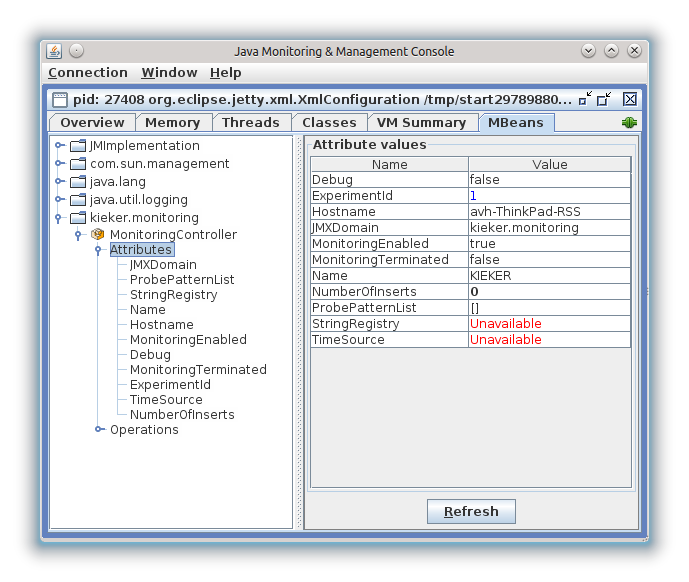
\includegraphics[scale=0.362]{images/jmxbean-monitoringcontroller-attributes.png} % 0.485\textwidth
}\hspace{-0.5cm}%
\subfigure[Operations]{%
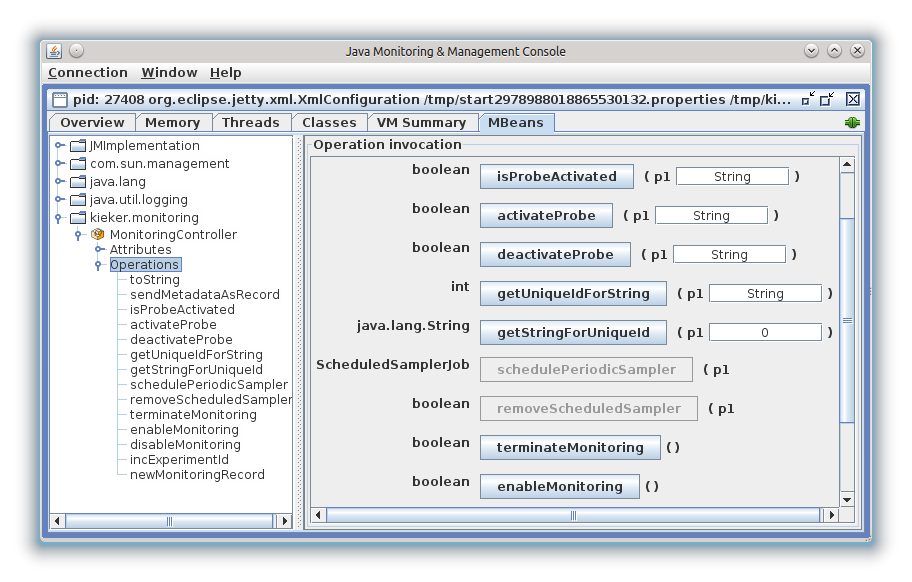
\includegraphics[scale=0.362]{images/jmxbean-monitoringcontroller-operations.png} % width=0.485\textwidth
}
\caption{Screenshots of the \class{jconsole} JMX client accessing the \class{MonitoringController}'s %
attributes and operations via the MBean interface. %
}
\label{fig:monitoringController:MBean:jconsole}
\end{figure}

In order to enable JMX MBean access to the \class{MonitoringController}, the corresponding configuration properties must be set to \textit{true} (listing below). %
The \file{\monitoringPropertiesFile} includes additional JMX-related configuration properties. \\

\setPropertiesListing
\begin{lstlisting}
## Whether any JMX functionality is available
kieker.monitoring.jmx=true
...

## Enable/Disable the MonitoringController MBean
kieker.monitoring.jmx.MonitoringController=true
...
\end{lstlisting}

For remote access to the server, set \textit{kieker.monitoring.jmx.remote=true}. In this case it is recommended to set \textit{com.sun.management.jmxremote.authenticate=true} as well. More information can be found on Oracle's JMX Technology Home Page~\cite{JMX-Website}.


\section{\KiekerMonitoringPart{} Configuration}\label{sec:monitoring:configuration}

\KiekerMonitoringPart{} instances can be configured by properties files, %
\class{Configuration} objects, and by passing property values as %
JVM arguments. If no configuration is specified, a default %
configuration is being used. %
Appendix~\ref{sec:appdx:monitoringproperties} lists this default %
configuration with a documentation of all available properties. %
The default configuration properties file, which %
can be used as a template for custom configurations, is provided by the file %
\file{\kiekerExampleMonitoringProperties} in the directory \dir{\KiekerDir/examples/} of %
the binary release (see Section~\ref{sec:example:downloadInstall}). %


\subsection*{Configurations for Singleton Instances}

In order to use a custom configuration file, its location needs to be passed to %
the JVM using the parameter \textit{kieker.monitoring.configuration} as follows:

\setBashListing
\begin{lstlisting}[caption=,label=lst:monitoringPropertiesPassedToJVM]
#\lstshellprompt# java  #\textbf{-Dkieker.monitoring.configuration=}#<ANY-DIR>/my.kieker.monitoring.properties #[\ldots]#
\end{lstlisting}

\noindent Alternatively, a file named \file{kieker.monitoring.properties} %
can be placed in a directory called \dir{META-INF/} located in the classpath. %
The available configuration properties can also be passed as JVM %
arguments, e.g., \lstinline{-Dkieker.monitoring.enabled=true}. %

\subsection*{Configurations for Non-Singleton Instances}

The class \class{Configuration} provides factory methods to create %
\class{Configuration} objects according to the default configuration %
or loaded from a specified properties file: \method{createDefaultConfiguration}, %
\method{createConfigurationFromFile}, and \method{createSingletonConfiguration}. %
Note, that JVM parameters are only evaluated when using the factory method %
\method{createSingletonConfiguration}. %
The returned \class{Configuration} objects can be adjusted by setting %
single property values using the method \method{setProperty}. %

\section{Monitoring Records}\label{sec:componentsMonitoring:monitoringRecords}

Monitoring records are objects that contain the monitoring data, as mentioned %
in the previous chapters. Typically, an instance of a monitoring record is %
constructed in a monitoring probe (Section~\ref{sec:monitoring:probe}), %
passed to the monitoring controller (Section~\ref{sec:componentsMonitoring:monitoringController}), %
serialized and deserialized by a monitoring %
writer (Section~\ref{sec:monitoring-log-writers}) and a
monitoring reader, and provided to analysis filters (Section~\ref{sec:analysis:controller}). %
Figure~\ref{fig:KiekerCommunicationDiagram} illustrates this life cycle of a monitoring %
record. %

In Chapter~\ref{chap:example}, we've already introduced and used the monitoring %
record type \class{OperationExecutionRecord}. \Kieker{} allows to use custom %
monitoring record types. Corresponding classes must implement the %
interface \class{IMonitoringRecord} shown in Figure~\ref{sec:monitoringrecord:interfacesAndImplementingClasses}. %
The methods \method{initFromArray}, \method{toArray}, \method{getValueTypes} %
are used for serialization and deserialization of the monitoring data contained %
in the record. Alternatively---in order to support the definition of immutable record types---the %
marker interface \class{IMonitoringRecord.Factory} needs to be implemented, requiring the %
implementation of (i)~the \method{toArray} method (as before), (ii)~a %
constructor accepting a values array, and (iii)~a public static \method{TYPES} %
field. The method \method{setLoggingTimestamp} is used by the monitoring controller to %
store the date and time when a record is received by the controller. %
The method \method{getLoggingTimestamp} can be used during analysis to retrieve %
this value. \KiekerMonitoringPart{} provides the abstract class %
\class{AbstractMonitoringRecord} (Figure~\ref{sec:monitoringrecord:interfacesAndImplementingClasses}) %
which already implements the methods to maintain the logging timestamp.

\begin{figure}[ht]\centering
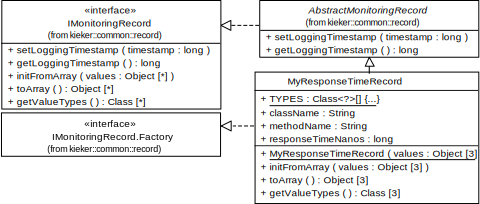
\includegraphics[scale=0.75]{images/kieker_MyRTRecord-modified}
\caption{Class diagram with the \class{IMonitoringRecord} and \class{IMonitoringRecord.Factory} interfaces, the abstract %
class \class{AbstractMonitoringRecord}, and a custom monitoring record type %
\class{MyResponseTimeRecord}}
\label{sec:monitoringrecord:interfacesAndImplementingClasses}
\end{figure}

%  \pagebreak

\noindent In order to use the abstract class for implementing your own monitoring record type, you need to:

\begin{enumerate}
\item Create a class that extends \class{AbstractMonitoringRecord}
\item  and
\begin{enumerate}
\item Override the methods \method{initFromArray}, \method{toArray}, \method{getValueTypes}
\item For immutable record types: implement \class{IMonitoringRecord.Factory}, a constructor %
with a single \class{Object[]} argument, and a public static \method{TYPES} field. %
In this case, \method{initFromArray} (which is not called by the framework then) should %
throw an \class{UnsupportedOperationException}.
\end{enumerate}
\end{enumerate}

\noindent The class \class{MyResponseTimeRecord}, shown in the class diagram in %
Figure~\ref{sec:monitoringrecord:interfacesAndImplementingClasses} and in %
Listing~\ref{listing:MyRecord}, is an example of a custom monitoring record type %
that can be used to monitor response times of method executions. %
Implementing \class{IMonitoringRecord.Factory}, \class{MyResponseTimeRecord} is %
an immutable type, i.e., it includes only final fields. %

\enlargethispage{1cm}

% \pagebreak 

\ % pushing the method initFromArray in the listing to the following page

\setJavaCodeListing
\lstinputlisting[caption=MyResponseTimeRecord.java, label=listing:MyRecord,firstline=27,firstnumber=27]{\customComponentsBookstoreApplicationDir/src/kieker/examples/userguide/ch3and4bookstore/MyResponseTimeRecord.java}

% \pagebreak

\section{Monitoring Probes}\label{sec:monitoring:probe}

The probes are responsible for collecting the monitoring data and passing it %
to the monitoring controller. %
In Chapter~\ref{sec:example:monitoring}, we have already demonstrated how to %
manually instrument a Java application. Listing~\ref{listing:cuttingBookstore} %
shows a similar manual monitoring probe, which uses the monitoring record type %
\class{MyResponseTimeRecord} defined in the previous Section~\ref{sec:componentsMonitoring:monitoringRecords}.

% Make sure that this listing will be modified, once the sourcecode changes!!!
% It must show the whole monitoring of the bookstorecall, from getting the first time to persisting of the record!!
% \pagebreak
\lstinputlisting[firstline=32, lastline=40, firstnumber=32, caption=Excerpt from Bookstore.java, label=listing:cuttingBookstore]{\customComponentsBookstoreApplicationDir/src/kieker/examples/userguide/ch3and4bookstore/Bookstore.java}

\noindent In order to avoid multiple calls to the \method{getInstance} method of the %
\class{MonitoringController} class, singleton instances should be stored %
in a final static variable, as shown in Listing~\ref{listing:cuttingBookstore:finalStaticController}.

\enlargethispage{1cm}

\lstinputlisting[firstline=24, lastline=25, firstnumber=24, caption=Singleton instance of the monitoring controller stored in a final static variable (excerpt from Bookstore.java), label=listing:cuttingBookstore:finalStaticController]{\customComponentsBookstoreApplicationDir/src/kieker/examples/userguide/ch3and4bookstore/Bookstore.java}

\noindent When manually instrumenting an application, the monitoring probe is implemented %
by mixing monitoring logic with business logic, which is often not desired since %
the resulting code is hardly maintainable. %
Many middleware technologies, such as Java~EE Servlet~\cite{JavaServletTechnology-WebSite}, %
Spring~\cite{Spring-WebSite}, and %
Apache~CXF~\cite{CXF-WebSite} provide interception/AOP~\cite{Kiczales1997} interfaces %
which are well-suited to implement monitoring probes. AspectJ~\cite{AspectJ-WebSite} allows to %
instrument Java applications without source code modifications. %
Chapter~\ref{chap:aspectJ} describes the \Kieker{} probes based on these technologies allowing to %
monitor trace information in distributed applications.

\section{Monitoring Writers}\label{sec:monitoring-log-writers}

Monitoring writers serialize monitoring records to the monitoring log/stream and  % and persist the recorded informations into files, databases etc. %
must implement the interface \class{IMonitoringWriter}. The monitoring %
controller passes the received records to the writer by calling the method %
\method{newMonitoringRecord}. Writers can use the methods to serialize the %
record contents, as described in Section~\ref{sec:componentsMonitoring:monitoringRecords}.

% This is the diagram with the hierarchy of the writers.
\begin{figure}[b]%[H]
	\begin{centering}
		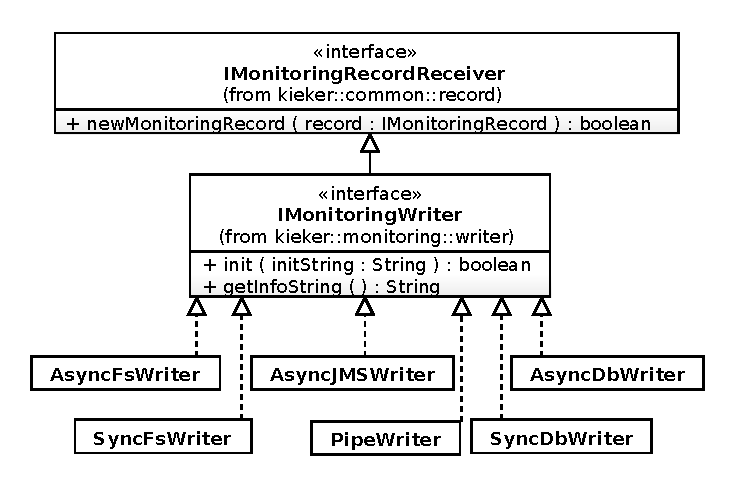
\includegraphics[scale=0.7]{images/kieker_writerimplsuserguide-modified}
		\caption{Interface \class{IMonitoringWriter} and  the implementing classes}
		\label{figure:monitoringLogWritersHierarchy}
	\end{centering}
\end{figure}

Figure~\ref{figure:monitoringLogWritersHierarchy} shows the monitoring writers %
already implemented in \KiekerMonitoringPart{}. The available properties for the %
included writers are well-documented in the %
example configuration file (see Appendix~\ref{sec:appdx:monitoringproperties}). %

% \enlargethispage{1.2cm}

Different writers can be used %
to store monitoring records to filesystems and databases respectively (e.g., \class{AsciiFileWriter}, %
\class{SyncFsWriter}, \class{AsyncDbWriter}, and \class{SyncDbWriter}). %
The variants with the prefix \class{Async} are implemented using asynchronous %
threads that decouple the I/O operations from the control flow of the %
instrumented application. %
The \class{AsciiFileWriter} is the default writer that has already been used in %
Section~\ref{sec:example:monitoring}. %
Please note that the database writers are currently in a prototype stage and
that they should be used with care. %
The \class{PrintStreamWriter} simply sends the String representation of incoming %
records to the standard output or standard error streams, which can be helpful %
for debugging purposes.

The \class{JmsWriter} and \class{JmxWriter} write records to a JMS %
(Java Messaging Service~\cite{JMS-WebSite}) queue and JMX (Java Management %
Extensions~\cite{JMX-Website}) queue respectively. The \class{PipeWriter} %
allows to pass records via in-memory record streams (named pipes). %
These writers allow to implement on-the-fly analysis in distributed systems, i.e., analysis while %
continuously receiving new monitoring data from an instrumented application potentially %
running on another machine. A more detailed description of how to use the \class{JmsWriter} %
can be found in Appendix~\ref{appendix:usingJMS}. %

\noindent Listing~\ref{listing:MyWriter} %on page~\pageref{listing:MyWriter} 
shows %
a custom writer \class{MyPipeWriter} which uses a named pipe to %
write the given records into a buffer located in the memory. The source code of %
the class \class{MyPipe} is listed in Appendix~\ref{appendix:pipeListings}. %

\setJavaCodeListing
\lstinputlisting[caption=MyPipeWriter.java, label=listing:MyWriter,firstline=23,firstnumber=23]{\customComponentsBookstoreApplicationDir/src/kieker/examples/userguide/ch3and4bookstore/MyPipeWriter.java}

% \pagebreak

\pagebreak

\noindent The monitoring writer to be used is selected by the %
\KiekerMonitoringPart{} configuration property (Section~\ref{chap:componentsMonitoring}) %
\textit{kieker.monitoring.writer}. Writer-specific configuration properties %
can be provided by properties prefixed by the fully-qualified writer classname.  %
Listing~\ref{lst:monitoringwriter:MyWriter} demonstrates how to use the custom %
writer \class{MyPipeWriter} defined above. In this example, the pipe name is %
passed as the property value \textit{pipeName}.

\setPropertiesListing
\lstinputlisting[caption={Configuration of the custom writer \class{MyPipeWriter}},label=lst:monitoringwriter:MyWriter,firstline=5,firstnumber=5,lastline=6]%
{\customComponentsBookstoreApplicationDir/src-resources/META-INF/kieker.monitoring.properties}

\enlargethispage{1cm}

\noindent As the data structure of this kind of monitoring stream, we created a %
class \class{PipeData} in order to demonstrate the use of the \method{toArray} and %
\method{initFromArray} (in Section~\ref{sec:analysis:reader}) methods. %
A \class{PipeData} object holds a logging timestamp and an \class{Object} array %
containing the serialized record data. %
Appendix~\ref{appendix:pipeListings} includes a source code listing of this class. %
Alternatively, we could have used \class{IMonitoringRecord} as the data structure %
used by the pipe. This is the way, \Kieker{}'s \class{PipeWriter} works. %

  %%%%%%%%%%%%%%%%%%%%%%%%%%%%%%%%%%%%%%%%%
% Kieker Analysis Component
%
% $Date$
% $Rev$:
% $Author$

\chapter{\KiekerAnalysisPart{} Component}\label{chap:componentsAnalysis}

\NOTIFYBOX{The Java sources of this chapter, as well as a pre-compiled binary, %
can be found in the %
\file{\customComponentsBookstoreApplicationReleaseDirDistro{}/} directory of the %
binary release.}

\section{Pipe-and-Filter Framework and Included Plugins}\label{sec:analysis:controller}

\KiekerAnalysisPart{} provides a framework to define and execute pipe-and-filter %
architectures of analysis plugins, i.e., monitoring readers and analysis filters, %
as well as repositories. %
This section describes how to use and develop readers, filters, and %
repositories. The description is based on the example %
pipe-and-filter architecture shown in Figure~\ref{fig:example:pipe-and-filter}. The custom monitoring reader %
\class{MyPipeReader}, which corresponds to the writer developed in Section~\ref{sec:monitoring-log-writers}, %
sends records to the connected custom filter \class{MyResponseTimeFilter}. %
This filter accepts only events of the record type \class{MyResponseTimeRecord},
developed in Section~\ref{sec:componentsMonitoring:monitoringRecords}. %
The \class{MyResponseTimeFilter} classifies incoming \class{MyResponseTimeRecord}s %
based on whether they satisfy or exceed a configured threshold and passes them %
to the respective output ports, \method{validResponseTimes} or \method{invalidResponseTimes}. %
Two instances of a second custom filter, \class{MyResponseTimeOutputPrinter}, %
print the received records to the standard output stream.

\begin{figure}
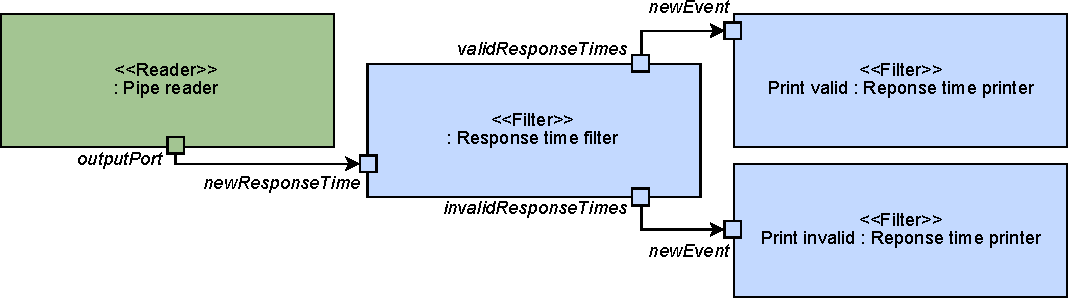
\includegraphics[width=\textwidth]{images/example-pipe-and-filter}
\caption{Example pipe-and-filter configuration}
\label{fig:example:pipe-and-filter}
\end{figure}

%  requires a monitoring reader %
% (Section~\ref{sec:analysis:reader}) and at least %
% one monitoring record consumer plugin (Section~\ref{sec:analysis:consumer}). %
% In addition to the monitoring record consumer plugin, %
% other analysis plugins can be registered. %

\begin{figure}\centering
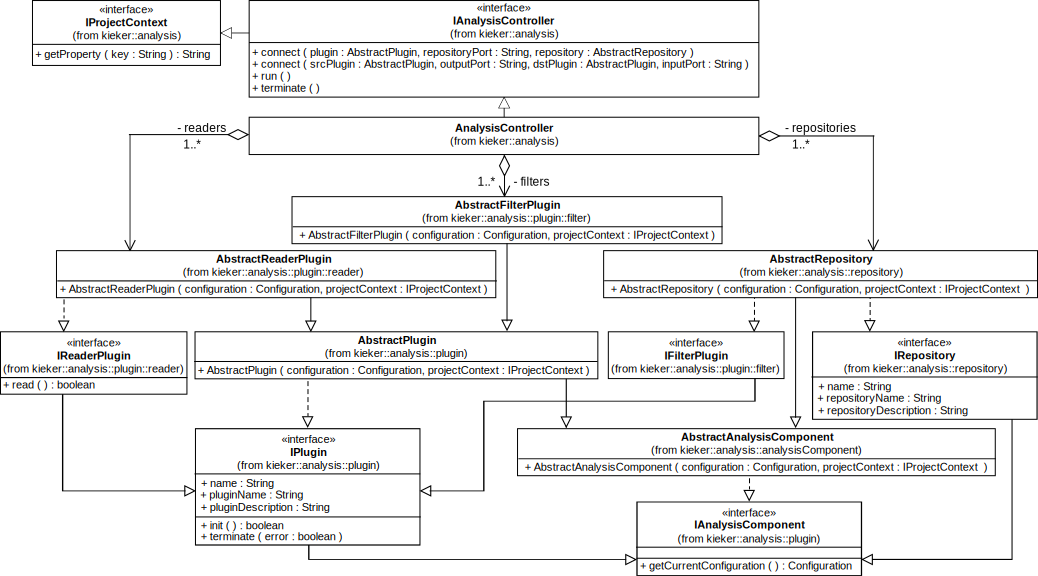
\includegraphics[width=\textwidth]{images/kieker_AnalysisControlleruserguide-modified}
\caption{Class diagram showing important \KiekerAnalysisPart{} types and their relationship}
\label{fig:analysisController:classdiagram}
\end{figure}

% \pagebreak

\noindent Figure~\ref{fig:analysisController:classdiagram} shows the class diagram %
with the important \KiekerAnalysisPart{} classes and their relationships. %
Note that only the most important methods are included. 
An analysis with \KiekerAnalysisPart{} is set up and executed employing %
the class \class{AnalysisController}. %
Setting up and running an analysis with \KiekerAnalysisPart{} requires the %
following steps to be performed, as sketched in Section~\ref{sec:example:analysis} already:

\enlargethispage{1.2cm}

\medskip

\begin{compactenum}
\item Creating an instance of the \class{AnalysisController} class
\item Creating monitoring readers, filters, and repositories.
\item Connecting plugins to other plugins and to repositories (\method{connect})
\item Starting the analysis instance (\method{run}).
\end{compactenum}

\medskip

\noindent On invocation of the \method{run} method, the \class{AnalysisController} %
calls the \method{init} method of all filter plugins allowing them to initialize. %
Then, it starts the configured monitoring readers by calling its \method{read} %
method. Plugins send data via their output ports to connected input ports of other
plugins. Being the source in a pipe-and-filter architecture, readers don't have %
input ports. Plugins can be connected to repositories, which may provide %
shared services, such as managed access to a common architectural model %
of the analyzed system. As soon as all readers have returned from the execution of their \method{read}
methods, the method \method{terminate} of each registered plugin is called by the %
\class{AnalysisController}. \KiekerAnalysisPart{} configurations can be saved %
to a \class{.kax} file by calling the \class{AnalysisController}'s \method{saveToFile} method. %
The \class{AnalysisController} provides a constructor which accepts the %
file system location of a \class{.kax} file to load the configuration from. %
See Appendix~\ref{appendix:wrapperScripts:kaxRun} and~\ref{appendix:wrapperScripts:kaxViz} %
for included tools/scripts which execute and visualize \class{.kax} files.
 %
In order to support the asynchronous execution of the \class{AnalysisController} instance, %
we provide the \class{AnalysisControllerThread} class.

\subsection{Programmatic Creation of Pipe-and-Filter Architectures}\label{sec:analysis:programmaticCreation}

To give a first impression of the programmatic %
instantiation, configuration, and connection of plugins, Listing~\ref{listing:StarterInitConnect} %
demonstrates this procedure for the example, using \class{MyPipeReader} and %
\class{MyResponseTimeFilter}, according to Figure~\ref{fig:example:pipe-and-filter}.

The configuration for the \class{MyPipeReader} is created in lines~51--52. %
Using this configuration, the reader is created in line~53. Similarly, %
lines~56--62 initialize the \class{MyResponseTimeFilter}. The reader's output is connected %
to the filter's input in line~63. %
The entire programmatic creation of the pipe-and-filter architecture shown %
in Figure~\ref{fig:example:pipe-and-filter}, can be found in the example  %
file \file{Starter.java}.

\medskip

\setJavaCodeListing
\lstinputlisting[caption=Initializing and connecting the example reader and filter (Starter.java),label=listing:StarterInitConnect,firstline=47, lastline=63, firstnumber=47]%
{\customComponentsBookstoreApplicationDir/src/kieker/examples/userguide/ch3and4bookstore/Starter.java}

\enlargethispage{0.5cm}

\subsection{Monitoring Reader Plugins}

% Warning-tag for the reader-writer-thing
The monitoring readers are the direct counterpart to the monitoring %
writers. While writers receive records and write them into files or other kinds %
of monitoring logs/streams, readers deserialize monitoring data and provide it as %
\class{IMonitoringRecord} instances.

\begin{figure}\centering
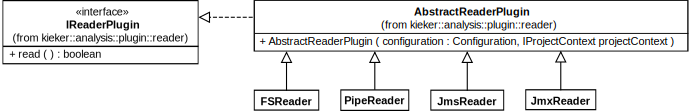
\includegraphics[scale=0.7]{images/kieker_readerimplsuserguide-modified}
\caption{Monitoring reader plugins included with \Kieker{}}
\label{Figure:ReaderHierarchy}
\end{figure}

% \pagebreak

% \
%
% \WARNBOX{This means that whenever a new writer is implemented, a corresponding reader has to be implemented as well. If one want for example to store the recorded informations in a database, one should be capable of reading these saved informations from the database again.}
%
% \

% \enlargethispage{1cm}

\noindent There are already some readers implemented in \Kieker,  as shown in the %
class diagram in Figure \ref{Figure:ReaderHierarchy}. %
The \class{FSReader} has already been used in Section~\ref{sec:example:analysis}. %
A brief description of how to use the \class{JmsReader} can be found in Appendix~%
\ref{appendix:usingJMS}. 
Like each plugin, readers are configured via properties, as used in Section~%
\ref{sec:analysis:programmaticCreation} and detailed in Section~%
\ref{sec:analysis:configuration}.

\subsection{Filter Plugins}

Filter plugins receive events (Java objects) via input ports from other %
plugins and implement analyses or visualizations based on these events. %
\Kieker{} already includes some basic filter plugins. For example, the %
\class{CountingFilter} and  \class{TeeFilter} forward incoming events %
to their output ports. The \class{CountingFilter} additionally provides the %
current number of received records via a second output port. The \class{TeeFilter} %
additionally prints incoming events to an output stream, which may be %
the standard output, standard error, a logger, or a file. %
A \class{TimestampFilter} and a \class{TypeFilter} filter incoming records by %
timestamp and by type, respectively. A \class{TraceIdFilter} filters incoming %
trace events (e.g., \class{OperationExecutionRecord}s, see Section~%
\ref{chap:example}) by trace ID. Additional filters for trace analysis, %
architecture reconstruction and visualization are included as part of %
the \KiekerTraceAnalysis{} tool, presented in Chapter~\ref{chap:aspectJ}. %
Like each plugin, filters are configured %
via properties, as used in Section~\ref{sec:analysis:programmaticCreation} and %
detailed in Section~%
\ref{sec:analysis:configuration}. %

% \pagebreak
% \setJavaCodeListing
%\lstinputlisting[caption=MyReponseTimeConsumer.java,label=lst:MyReponseTimeConsumer,firstline=21,firstnumber=21]{\customComponentsBookstoreApplicationDir/src/kieker/examples/userguide/ch3and4bookstore/MyResponseTimeConsumer.java}

% The following Listing~\ref{listing:AnalysisController} shows how to create and run an analysis %
% with these custom components:
%
% \setJavaCodeListing
% \lstinputlisting[caption=Code snippet setting up and running a \KiekerAnalysisPart{} instance (Starter.java),label=listing:AnalysisController,firstline=48, lastline=82, firstnumber=48]%
% {\customComponentsBookstoreApplicationReleaseDir/src/kieker/examples/userguide/ch3and4bookstore/Starter.java}

% \enlargethispage{1.2cm}

\subsection{Repositories}

Currently, \Kieker{} includes a single repository, \class{SystemModelRepository}, %
which is used by the \KiekerTraceAnalysis{} filters to update and query %
a component-based system model representing architectural entities %
and structures discovered while processing the incoming monitoring data. %
The development and use of repositories is detailed in Section~%
\ref{sec:analysis:repositories}. %

When using components of the \KiekerTraceAnalysis{}, make sure that write access to the %
\class{SystemModelRepository} is only triggered by readers. Some filters are terminated %
after the readers and expect the repository to be in a completed state.


\section{Developing Analysis Plugins and Repositories}\label{sec:analysis:plugins}

When implementing analysis plugins (i.e., readers or filters) and repositories, %
the classes \class{AbstractReaderPlugin}, \class{AbstractFilterPlugin}, or, %
respectively, \class{AbstractRepository} need to be extended %
(Figure~\ref{fig:analysisController:classdiagram}). %
Section~\ref{sec:analysis:configuration} describes how plugins and repositories %
can be configured via properties. %
Section~\ref{sec:analysis:pluginAnnotation} %
describes how to declare meta-information for plugins using %
dedicated annotations. %
Specific information on the development of custom filters, readers, and repositories %
are given in Sections~\ref{sec:analysis:filters}--\ref{sec:analysis:repositories}. %

% The monitoring record consumer plugins described in the following %
% Section~\ref{sec:analysis:consumer}, are special analysis plugins that receive %
% the monitoring records provided by the monitoring reader. %
% Starting with these monitoring record plugins, analysis plugins can be connected %
% in a pipe-and-filter style to implement more complex analyses. %
% \Kieker{} provides input and output port interfaces and implementing classes %
% to implement such analyses. See the documentation of the classes \class{AbstractInputPort} %
% and \class{OutputPort} for details. \KiekerTraceAnalysis{} is implemented %
% based on this pattern.

\subsection{Configuration}\label{sec:analysis:configuration}

\noindent According to the %
configuration of the \KiekerMonitoringPart{} components (see Section~\ref{sec:monitoring:configuration}),
plugins and repositories are configured via \class{Configuration} objects. Classes must %
provide a public constructor, accepting a \class{Configuration} and an \class{IProjectContext} (normally the \class{IAnalysisController} instance) object as %
its only arguments. It is important to invoke the constructor of the super class. %
The configuration properties accepted by a plugin or repository should be provided via \class{public static} %
constants with prefix \method{CONFIG\_PROPERTY\_NAME\_} in order to ease the %
programmatic initialization of plugins (Section~\ref{sec:analysis:programmaticCreation}). %
For the example filter \class{MyResponseTimeFilter},
Listing~\ref{listing:MyResponseTimeFilterConstructor} shows the constructor,
the configuration property, and the corresponding member value obtained from the %
configuration.

\setJavaCodeListing
\lstinputlisting[firstline=44, firstnumber=44, lastline=52, caption={Plugin constructor accepting a \class{Configuration} and an \class{IProjectContext} object}, label=listing:MyResponseTimeFilterConstructor]%
{\customComponentsBookstoreApplicationDir/src/kieker/examples/userguide/ch3and4bookstore/MyResponseTimeFilter.java}

\noindent Additionally, the %
current configuration must be provided via the method %
\method{getCurrentConfiguration}. Please note that the returned configuration %
should be sufficient to initialize the plugin or repository via the mentioned constructor. %
The \class{AnalysisController} uses the \method{getCurrentConfiguration} to %
save the pipe-and-filter configuration. Listing~\ref{listing:MyResponseTimeFilterEventsToOutput} %
shows how the methods are implemented for the example filter \class{MyResponseTimeFilter}. %

\enlargethispage{1cm}

\setJavaCodeListing
\lstinputlisting[firstline=69, firstnumber=69, lastline=74, caption={Plugin returning its current configuration}, label=listing:MyResponseTimeFilterEventsToOutput]%
{\customComponentsBookstoreApplicationDir/src/kieker/examples/userguide/ch3and4bookstore/MyResponseTimeFilter.java}

\noindent The declaration of the available properties and their default values within a plugin is shown in section~\ref{sec:analysis:pluginAnnotation}, as this is done with annotations.

% \pagebreak

\subsection{@Plugin Annotation and Output Ports}\label{sec:analysis:pluginAnnotation}

\noindent The \class{@Plugin} class annotation is used to define a %
plugin name, a description, and the lists of output ports and configuration %
properties with default values. %
Listing~\ref{listing:MyResponseTimeFilterPluginAnnotationOutputs} shows the %
\class{@Plugin} annotation for the example filter.

\enlargethispage{1cm}

If the \class{@Plugin} annotation is not present for a plugin, the \method{name} %
defaults to the plugin's (simple) classname, the \method{description} defaults %
to the empty string, and the list of output ports is empty. These default values %
are also used in case a respective attribute is omitted. %
Note that the name is not required to be a unique among filters; it is simply %
used for descriptive purposes, such as in Figure~\ref{fig:example:pipe-and-filter}. %

Output ports are specified using the nested \class{@OutputPort} annotation. %
In addition to a name and a description for the output port, a list of event %
types can be specified. Note that in this case, the name is mandatory and must %
be unique for a plugin, as it is used for connecting input and output ports. %
The list of event types defaults to a list including only \class{Object.class}. %
The output port names should be provided as a \class{public static} constant %
with prefix \method{OUTPUT\_PORT\_NAME\_}, in order to ease the programmatic %
connection of readers and filters, as described in %
Section~\ref{sec:analysis:programmaticCreation}. Repositories required by %
filters are also specified as part of the \class{@Plugin} annotation. %
This is detailed in Section~\ref{sec:analysis:repositories}. %

\setJavaCodeListing
\lstinputlisting[firstline=27, firstnumber=27, lastline=40, caption={@Plugin annotation for the example plugin \class{MyResponseTimeFilter}}, label=listing:MyResponseTimeFilterPluginAnnotationOutputs]%
{\customComponentsBookstoreApplicationDir/src/kieker/examples/userguide/ch3and4bookstore/MyResponseTimeFilter.java}

\noindent Plugins can send events to their output ports by calling the %
\method{deliver} method provided by the super class. The method expects the %
output port name and the event to be sent as arguments. Listing~%
\ref{listing:MyResponseTimeFilterDelivers} %
shows how the example filter plugin \class{MyResponseTimeFilter} delivers records %
to its two output ports declared in the \class{@Plugin} annotation.

% \pagebreak

\setJavaCodeListing
\lstinputlisting[firstline=61, firstnumber=61, lastline=65, caption={Plugin sending events to output ports}, label=listing:MyResponseTimeFilterDelivers]%
{\customComponentsBookstoreApplicationDir/src/kieker/examples/userguide/ch3and4bookstore/MyResponseTimeFilter.java}

Listing~\ref{listing:MyResponseTimeFilterPluginAnnotationOutputs} shows also how %
the properties are declared. Using the \class{@Property} annotation, it is possible to declare %
the existing properties. Each property has a default value which should be sufficient %
to initialize the plugin.%

The \class{@Plugin} annotation (as well as the later introduced \class{@Repository} annotation) contains %
furthermore the two fields \method{dependencies} and \method{programmaticOnly}. The first %
one offers the possibility to give a description of the needed dependencies for a plugin %
(other libraries e.g.). The latter marks whether the current plugin (or repository) is for %
programmatic purposes only, i.e., they are of little use in graphical analysis %
tools.

\subsection{Developing Monitoring Reader Plugins}\label{sec:analysis:reader}

\noindent Custom readers must extend the class %
\class{AbstractReaderPlugin} (see Figure~\ref{fig:analysisController:classdiagram}), %
and implement the methods \method{init}, \method{read}, and \method{terminate}, %
which are called by the \class{AnalysisController} to trigger the reader's initialization, %
reading, and termination. Like each plugin (Section~\ref{sec:analysis:configuration}), %
readers are configured via a constructor accepting a \class{Configuration} and an \class{IProjectContext} object %
as its only arguments; they must provide the current configuration %
via the implemented \method{getCurrentConfiguration} %
method. Readers start reading on invocation of the \method{read} method, %
providing the obtained records to connected filters via the output port(s) %
declared in the \class{@Plugin} annotation (Section~\ref{sec:analysis:pluginAnnotation}). %
The \method{read} method should be implemented synchronously, i.e., it should %
return after reading is finished or has been aborted via an invocation of the %
\method{terminate} method.

% If there is nothing on the pipe to be read, the reader waits 4 seconds at maximum before it terminates.
% \setJavaCodeListing
% \lstinputlisting[firstline=29, firstnumber=29, caption=MyPipeReader.java (excerpt), label=listing:MyReader,float]{\customComponentsBookstoreApplicationDir/src/kieker/examples/userguide/ch3and4bookstore/MyPipeReader.java}

\enlargethispage{1cm}

\setJavaCodeListing
\lstinputlisting[firstline=28, firstnumber=28, lastline=40, caption={@Plugin annotation for the example reader}, label=listing:MyPipeReaderPluginAnnotation]%
{\customComponentsBookstoreApplicationDir/src/kieker/examples/userguide/ch3and4bookstore/MyPipeReader.java}

Listing~\ref{listing:MyPipeReaderPluginAnnotation} shows the \class{@Plugin} %
annotation  of the example reader \class{MyPipeReader}. Reading monitoring %
records from the monitoring pipe introduced in the previous Chapter~%
\ref{sec:monitoring-log-writers}, the reader provides received monitoring %
records via its output port.

\noindent Listing~\ref{listing:MyPipeReaderInit} shows an excerpt of the \class{MyPipeReader}'s %
constructor. In this case, the reader reads the pipe name from the %
configuration and connects to the named pipe. Optionally, the reader can override the 
\method{init} method.

 \pagebreak

\setJavaCodeListing
\lstinputlisting[firstline=51, firstnumber=51, lastline=57, caption={Example reader's initialization in the constructor (excerpt)}, label=listing:MyPipeReaderInit]%
{\customComponentsBookstoreApplicationDir/src/kieker/examples/userguide/ch3and4bookstore/MyPipeReader.java}

% \pagebreak

\noindent Listing~\ref{listing:MyPipeReaderRead} shows the \class{MyPipeReader}'s %
\method{read} method. In this case, the reader polls the pipe for new records %
and forwards these to its output port.

\setJavaCodeListing
\lstinputlisting[firstline=60, firstnumber=60, lastline=80, caption={Example reader's \method{read} method}, label=listing:MyPipeReaderRead]%
{\customComponentsBookstoreApplicationDir/src/kieker/examples/userguide/ch3and4bookstore/MyPipeReader.java}

\vspace{-0.2cm}

\subsection{Developing Filter Plugins}\label{sec:analysis:filters}

Custom filters must extend the class \class{AbstractFilterPlugin}. %
In addition to providing meta information, including output ports, via the %
\class{@Plugin} annotation %
(Section~\ref{sec:analysis:pluginAnnotation}), as well as implementing a constructor %
and the getter for handling the \class{Configuration} (Section~\ref{sec:analysis:configuration}), %
filters may override the methods \method{init} and %
\method{terminate}, implementing initialization and cleanup tasks. %
The \class{@Plugin} annotation of the example filter \class{MyResponseTimeFilter} %
was shown in Listing~\ref{listing:MyResponseTimeFilterPluginAnnotationOutputs} already.

% \enlargethispage{1cm}

Filters receive events via methods marked with the \class{@InputPort} %
annotation. These methods must accept a single argument, which has to be %
a super type of the set of accepted event types declared in the respective %
\class{@InputPort} annotation's \method{eventTypes}. %
In addition to an optional \method{description}, each \class{@InputPort} %
must have a \method{name}, which is unique for this filter. The input port names %
should be provided as a \class{public static} constants %
with prefix \method{INPUT\_PORT\_NAME\_}, in order to ease the programmatic %
connection of readers and filters, as described in %
Section~\ref{sec:analysis:programmaticCreation}. %
Listing~\ref{listing:MyResponseTimeFilterInputPort} shows the declaration %
of the input port provided by the example plugin \class{MyResponseTimeFilter}. %
The body of this method was shown in Listing~%
\ref{listing:MyResponseTimeFilterDelivers} already.

% \pagebreak

\setJavaCodeListing
\lstinputlisting[firstline=56, firstnumber=56, lastline=60, caption={@InputPort annotation for the example plugin's input method}, label=listing:MyResponseTimeFilterInputPort]%
{\customComponentsBookstoreApplicationDir/src/kieker/examples/userguide/ch3and4bookstore/MyResponseTimeFilter.java}

\subsection{Developing and Accessing Required Repositories}\label{sec:analysis:repositories}

Custom repositories must extend the class \class{AbstractRepository}. %
The \class{@Repository} annotation is used to provide a \method{name} %
and a \method{description} for a repository type. %
Listing~\ref{listing:RepositoryAnnotation} shows the \class{@Repository} annotation %
of the \class{SystemModelRepository}, which is included in \Kieker{} as part of the %
\KiekerTraceAnalysis{} tool. %

\enlargethispage{1cm}

\setJavaCodeListing
\lstinputlisting[firstline=43, firstnumber=43, lastline=46, caption={\class{@Repository} annotation of Kieker's \class{SystemModelRepository}}, label=listing:RepositoryAnnotation]%
{../../kieker-tools/src/kieker/tools/traceAnalysis/systemModel/repository/SystemModelRepository.java}

\noindent Plugins specify the list of required repositories in their %
\class{@Plugin} annotation. Repositories are connected to filter-provided %
repository ports. A plugin's repository ports are specified using the %
nested \class{@RepositoryPort} annotation, as depicted for a %
\KiekerTraceAnalysis{} filter in Listing~\ref{listing:RepositoryRequirementDeclaration}. %
Like for input and output port names, this name must be unique for the plugin %
and should be provided as a \class{public static} constant %
with prefix \method{REPOSITORY\_PORT\_NAME\_}, in order to ease the programmatic %
connection of repositories to readers and filters. %

\setJavaCodeListing
\lstinputlisting[firstline=40, firstnumber=40, lastline=41, caption={Declaration of required repositories in the @Repository annotation}, label=listing:RepositoryRequirementDeclaration]%
{../../kieker-tools/src/kieker/tools/traceAnalysis/filter/AbstractTraceAnalysisFilter.java}

\pagebreak

\noindent Plugins can access their connected repositories via the \method{getRepository} %
method provided by the super class, as shown in Listing~\ref{listing:RepositoryAccess}. %

\setJavaCodeListing
\lstinputlisting[firstline=161, firstnumber=161, lastline=162, caption={Accessing a repository within a plugin}, label=listing:RepositoryAccess]%
{../../kieker-tools/src/kieker/tools/traceAnalysis/filter/AbstractTraceAnalysisFilter.java}


  %%%%%%%%%%%%%%%%%%%%%%%%%%%%%%%%%%%%%%%%%
% Trace Analysis and Monitoring
%
% $Date$
% $Rev$:
% $Author$

\chapter{\KiekerTraceAnalysis{} Tool}\label{chap:aspectJ}

\KiekerTraceAnalysis{} implements the special feature of \Kieker{} allowing to %
monitor, analyze, and visualize (distributed) traces of method executions and %
corresponding timing information. For this purpose, it includes monitoring probes employing %
AspectJ~\cite{AspectJ-WebSite}, Java~EE Servlet~\cite{JavaServletTechnology-WebSite}, %
Spring~\cite{Spring-WebSite}, and Apache~CXF~\cite{CXF-WebSite} technology. %
Moreover, it allows to reconstruct and visualize architectural models of the %
monitored systems, e.g., as sequence and dependency diagrams. %

Section~\ref{chap:example} already introduced parts of the monitoring record %
type \class{OperationExecutionRecord}. \KiekerTraceAnalysis{} uses this record %
type to represent monitored executions and associated trace and session information. %
Figure~\ref{fig:OperationExecutionRecordClassDiagramComplete} shows a class diagram %
with all attributes of the record type \class{OperationExecutionRecord}. %
The attributes \method{className}, \method{operationName}, %
\method{tin}, and \method{tout} have been introduced before. %
The attributes \method{traceId} and \method{sessionId} are used to store %
trace and session information; \method{eoi} and \method{ess} contain control-flow %
information needed to reconstruct traces from monitoring data. %
For details on this, please refer to our technical %
report~\cite{vanHoornRohrHasselbringWallerEhlersFreyKieselhorst2009TRContinuousMonitoringOfSoftwareServicesDesignAndApplicationOfTheKiekerFramework}.

\begin{figure}[hb]\centering
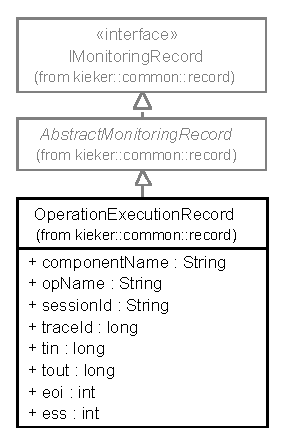
\includegraphics[scale=0.8]{images/kieker_OperationExecutionRecord-complete-modified}%
\caption{The class diagram of the operation execution record}
\label{fig:OperationExecutionRecordClassDiagramComplete}
\end{figure}

\enlargethispage{1cm}

\noindent Section~\ref{sec:traceMonitoring} describes how to instrument Java %
applications for monitoring trace information. %
It presents the technology-specific probes provided by \Kieker{} for this %
purpose---with a focus on AspectJ. %
Additional technology-specific probes can be implemented based on the existing %
probes. %
Section~\ref{sec:traceAnalysisTool} presents the %
tool which can be used to analyze and visualize the recorded trace %
data.  Examples for the available analysis and visualization outputs %
provided by \KiekerTraceAnalysis{} are presented in %
Section~\ref{sec:traceAnalysisExamples}.

\section{Monitoring Trace Information}\label{sec:traceMonitoring}

The following Sections describe how to use the monitoring probes based on %
AspectJ (Section~\ref{sec:traceAnalysis:instr:AspectJ}), %
the Java Servlet~API (Section~\ref{sec:traceAnalysis:instr:servlet}), %
the Spring Framework (Section~\ref{sec:traceAnalysis:instr:spring}), and %
Apache~CXF (Section~\ref{sec:traceAnalysis:instr:cxf}) provided %
by \Kieker{}. %

\subsection{AspectJ-Based Instrumentation}\label{sec:traceAnalysis:instr:AspectJ}

AspectJ~\cite{AspectJ-WebSite} allows to weave code into the byte code of %
Java applications and libraries without requiring manual modifications of the %
source code. %
\Kieker{} includes the AspectJ-based monitoring probes %
\class{OperationExecutionAspectAnnotation}, %
\class{OperationExecutionAspectAnnotationServlet}, %
\class{OperationExecutionAspectFull}, and %
\class{OperationExecutionAspectFullServlet} %
which can be woven into Java applications at compile time and load time. %
These probes monitor method executions and corresponding %
trace and timing information. The probes with the postfix \class{Servlet} %
additionally store a session identifier within the \class{OperationExecutionRecord}. %
When the probes with name element \class{Annotation} are used, %
methods to be monitored must be annotated by the \Kieker{} %
annotation \class{@OperationExecutionMonitoringProbe}. %
This section demonstrates how to use the AspectJ-based probes to monitor %
traces based on the Bookstore application from Chapter~\ref{chap:example}. %

% \enlargethispage{1.0cm}

\NOTIFYBOX{The Java sources of the example presented in %
this section, as well as a pre-compiled binary, can be found in the %
\file{\aspectJBookstoreApplicationReleaseDirDistro{}/} directory of the %
binary release.}

% \

% This chapter will show in Section~\ref{sec:aspectJ:annotation} how
% to use AspectJ to mark methods to be monitored with a simple annotation
% in order to avoid the manual monitoring as seen in Chapter~\ref{chap:example}
% and \ref{chap:componentsMonitoring}. Once the methods are marked, the AspectJ-Weaver-Agent
% will surround the calls with the necessary code during runtime, similar
% to the manually inserted instrumentation code used in Section~\ref{sec:example:monitoring}.
% An alternative solution will be shown as well in Section~\ref{sec:aspectJ:fullweaving}, %
% where the methods to be instrumented are specified using an external configuration file %
% without requiring source code modifications. Both solutions
% can be used to reconstruct architectural views and to perform trace
% analyses. The result of both will be diagrams similar to sFigure~\ref{fig:bookstore:classAndSequenceDiagrams}.

% The idea of weaving the monitoring-code into the ``plain'' code
% during compile-time seems to suggest itself, but
% in this chapter it
% is only shown how to perform the so called load-time-weaving - the
% weaving during runtime.%, which is more flexible than the compile-time-weaving.

\begin{figure}[H]
\begin{graybox}
\dirtree{%
.1 \DirInDirTree{examples/}. %\DTcomment{The root directory of the project}.
.2 \DirInDirTree{userguide/}.
.3 \DirInDirTree{ch5--trace-monitoring-aspectj/}.
.4 \DirInDirTree{build/}\DTcomment{Directory for the Java class files}.
.5 \DirInDirTree{libs/}.
.6 BookstoreApplication.jar.
.4 \DirInDirTree{gradle/}.
.5 \DirInDirTree{wrapper/}\DTcomment{Directory for the gradle wrapper}.
.6 \ldots.
.4 \DirInDirTree{lib/} \DTcomment{Directory for the needed libraries}.
.5 \newFileDirInDirTree{\mainJarWeaver}.
.4 \DirInDirTree{src/}\DTcomment{Directory for the source code files}.
.5 \DirInDirTree{../ch5bookstore/}.
.6 Bookstore.java.
.6 BookstoreHostnameRewriter.java.
.6 BookstoreStarter.java.
.6 Catalog.java.
.6 CRM.java.
.4 \DirInDirTree{src-resources/}.
.5 \DirInDirTree{META-INF/}\DTcomment{Directory for the configuration files}.
.6 aop.xml.
.6 aop-event.xml.
.6 aop-full.xml.
.6 kieker.monitoring.adaptiveMonitoring.conf.
.6 \kiekerMonitoringProperties{}. 
.3 build.gradle.
.3 gradlew.
.3 gradlew.bat.
.3 README.txt.
}
\end{graybox}

\caption{The new directory structure of the Bookstore application}
\label{fig:bookstoreAOP:dirStructure}
\end{figure}

Figure~\ref{fig:bookstoreAOP:dirStructure} shows the directory used by the example of this section. %
The jar-file \file{\mainJarWeaver} already includes the \textit{AspectJ weaver}, %
which is registered with the JVM and weaves the monitoring instrumentation into %
the Java classes. It will be configured based on the configuration file %
\file{\file{\aopConfigFile}}, for which a working sample file is provided in the %
example's \dir{META-INF/} directory. Instead of registering the \file{\mainJarWeaver} %
as an agent to the JVM, the \file{\aspectJWeaverJar} can be used. In this case, %
the \file{\mainJar} needs to be added to the classpath.

\pagebreak

Once the necessary files have been copied to the example directory, the source code can be instrumented with the annotation
\class{OperationExecutionMonitoringProbe}. Listing~\ref{lst:BookstoreAspectJ} shows how the annotation is used.

\setJavaCodeListing
\lstinputlisting[caption=Bookstore.java, label=lst:BookstoreAspectJ,firstline=21,firstnumber=21]{\aspectJBookstoreApplicationDir/src/kieker/examples/userguide/ch5bookstore/Bookstore.java}

\noindent As a first example, each method of the Bookstore application will be annotated. The annotation can be used to instrument all methods except for constructors.

The \file{\aopConfigFile} file has to be modified to specify the classes to be considered for instrumentation by the AspectJ weaver. Listing~\ref{lst:aopConfigFileAnnotations} shows the modified configuration file.

\enlargethispage{1cm}
\setXMLListing
\lstinputlisting[caption=aop.xml, label=lst:aopConfigFileAnnotations]{\aspectJBookstoreApplicationDir/src-resources/META-INF/aop.xml}

\noindent Line~5 tells the AspectJ weaver to consider all classes inside the example package. %
AspectJ allows to use wild-cards for the definition of classes to %
include---e.g., \lstinline$<include within="bookstoreTracing.Bookstore*"/>$ to weave all %
classes with the prefix \class{Bookstore} located in a package \class{bookstoreTracing}.

Line~9 specifies the aspect to be woven into the classes. In this case, the \Kieker{} %
probe \class{OperationExecutionAspectAnnotation} is used. It requires that %
methods intended to be instrumented are annotated by %
\lstinline[language=Java]{@OperationExecutionMonitoringProbe}, as mentioned before.

Listings~\ref{lst:traceAnalysisCompileRunExample1} and %
\ref{lst:traceAnalysisCompileRunExample1Win} show how to compile and run the annotated %
Bookstore application. The \file{\aopConfigFile} must be located in a %
\dir{META-INF/} directory in the classpath---in this case the \dir{build/} directory. %
The AspectJ weaver has to be loaded as a so-called Java-agent. It weaves the %
monitoring aspect into the byte code of the Bookstore application. %
Additionally, a \file{\kiekerMonitoringProperties{}} is copied to the \dir{META-INF/} directory. %
This configuration file may be adjusted as desired (see Section~\ref{sec:monitoring:configuration}).

\


\setBashListing
\begin{lstlisting}[caption=Commands to compile and run the Bookstore under \UnixLikeSystems, label=lst:traceAnalysisCompileRunExample1]
#\lstshellprompt{}# mkdir build/META-INF
#\lstshellprompt{}# javac src/kieker/examples/userguide/ch5bookstore/*.java \
        -d build/ -classpath lib/#\mainJarWeaver{}#

#\lstshellprompt{}# cp src-resources/META-INF/aop.xml build/META-INF/
#\lstshellprompt{}# cp src-resources/META-INF/kieker.monitoring.properties build/META-INF/

#\lstshellprompt{}# java -#\textbf{javaagent}#:lib/#\mainJarWeaver{}# \
       -classpath build/ kieker.examples.userguide.ch5bookstore.BookstoreStarter
\end{lstlisting}

\begin{lstlisting}[caption=Commands to compile and run the annotated Bookstore under Windows, label=lst:traceAnalysisCompileRunExample1Win]
#\lstshellprompt{}# mkdir build\META-INF
#\lstshellprompt{}# javac src\kieker\examples\userguide\ch5bookstore\*.java
        -d build -classpath lib\#\mainJarWeaver{}#

#\lstshellprompt{}# copy src-resources\META-INF\aop.xml build\META-INF\
#\lstshellprompt{}# copy src-resources\META-INF\kieker.monitoring.properties build\META-INF\

#\lstshellprompt{}# java -#\textbf{javaagent}#:lib\#\mainJarWeaver{}#
       -classpath build\ kieker.examples.userguide.ch5bookstore.BookstoreStarter
\end{lstlisting}


\noindent After a complete run of the application, the monitoring files should appear in %
the same way as mentioned in Section~\ref{sec:example:monitoring} including the %
additional trace information. An example log of a complete run can be found in %
Appendix~\ref{sec:appendix:exampleConsoleOutputs:aspectJExample}.

\paragraph*{Instrumentation without annotations}%\label{sec:aspectJ:fullweaving}

AspectJ-based instrumentation without using annotations is quite simple. It is %
only necessary to modify the file \file{\aopConfigFile{}}, as shown %
in Listing~\ref{lst:aopConfigFileFull}.
\pagebreak
\setXMLListing
\lstinputlisting[caption=aop.xml, label=lst:aopConfigFileFull]{\aspectJBookstoreApplicationDir/src-resources/META-INF/aop-full.xml}

\noindent The alternative aspect \class{OperationExecutionAspectFull} is being %
activated in line~9. As indicated by its name, this aspect makes sure that every %
method within the included classes/packages will be instrumented and monitored. %
% The exact behavior can be controlled very exactly by using appropriate includes and excludes within the weaver-part of the configuration file. %
% For example,
Listing \ref{lst:aopConfigFileFull} demonstrates how to limit the %
instrumented methods to those of the class \class{BookstoreStarter}.

The commands shown in the Listings~\ref{lst:traceAnalysisCompileRunExample1} and %
\ref{lst:traceAnalysisCompileRunExample1Win} can again be used to compile and execute %
the example. Note that the annotations within the source code have no effect %
when using this aspect.

\

\WARNBOX{When using a custom aspect, it can be necessary to specify its %
classname in the \lstinline{include} directives of the \aopConfigFile{}.}

\subsection{Servlet Filters}\label{sec:traceAnalysis:instr:servlet}

The Java Servlet API~\cite{JavaServletTechnology-WebSite} includes the %
\class{javax.servlet.Filter} interface. It can be used to implement %
interceptors for incoming HTTP requests. %
\Kieker{} includes the probe %
\class{SessionAndTraceRegistrationFilter} which implements the %
\class{javax.servlet.Filter} interface. %
It initializes the session and trace information for incoming requests. %
If desired, it additionally creates an \class{OperationExecutionRecord} for each %
invocation of the filter and passes it to the \class{MonitoringController}.

% \enlargethispage{1.5cm}

Listing~\ref{lst:OperationExecutionRegistrationAndLoggingFilterInWebXML} %
demonstrates how to integrate the \class{SessionAndTraceRegistrationFilter} %
in the \file{web.xml} file of a web application.

The Java~EE Servlet container example described in Appendix~\ref{appendix:JavaEEServletExample} employs the %
\class{SessionAndTraceRegistrationFilter}.

\pagebreak

\setXMLListing
\lstinputlisting[firstline=50,lastline=61,firstnumber=50,%
caption=\class{SessionAndTraceRegistrationFilter} in a \file{web.xml} file,%
label=lst:OperationExecutionRegistrationAndLoggingFilterInWebXML]%
{\JavaEEServletExampleDir/jetty/webapps/jpetstore/WEB-INF/web.xml}


\subsection{Spring}\label{sec:traceAnalysis:instr:spring}

The Spring framework~\cite{Spring-WebSite} provides interfaces for intercepting %
Spring services and web requests. %
\Kieker{} includes the probes %
\class{OperationExecutionMethodInvocationInterceptor} and
\class{OperationExecutionWebRequestRegistrationInterceptor}. %
The \class{OperationExecutionMethodInvocationInterceptor} is similar to the %
AspectJ-based probes described in the previous section and monitors method %
executions as well as corresponding trace and session information. %
The \class{OperationExecutionWebRequestRegistrationInterceptor} intercepts %
incoming Web requests and initializes the trace and session data for this %
trace. If you are not using the \class{OperationExecutionWebRequestRegistrationInterceptor}, %
you should use one of the previously described Servlet filters to register %
session information for incoming requests %
(Section~\ref{sec:traceAnalysis:instr:servlet}).

See the Spring documentation for instructions how to add the interceptors %
to the server configuration.

\subsection{CXF SOAP Interceptors}\label{sec:traceAnalysis:instr:cxf}

The Apache~CXF framework~\cite{CXF-WebSite} allows to implement interceptors for web service calls, %
for example, based on the SOAP web service protocol. %
\Kieker{} includes the probes %
\class{OperationExecutionSOAPRequestOutInterceptor}, %
\class{OperationExecutionSOAPRequestInInterceptor}, %
\class{OperationExecutionSOAPResponseOutInterceptor}, and %
\class{OperationExecutionSOAPResponseInInterceptor} which can be used to %
monitor SOAP-based web service calls. %
Session and trace information is written to and read from the SOAP header of %
service requests and responses allowing to monitor distributed traces. %
See the CXF documentation for instructions how to add the interceptors %
to the server configuration.

\pagebreak

\section{Trace Analysis and Visualization}\label{sec:traceAnalysisTool}

\enlargethispage{0.5cm}

Monitoring data including trace information can be analyzed and visualized with the \KiekerTraceAnalysis{} tool which is included in the \Kieker{} binary as well.\\

\WARNBOX{
In order to use this tool, it is necessary to install two third-party programs:
\begin{enumerate}
\item \textbf{Graphviz} A graph visualization software which can be downloaded from \url{http://www.graphviz.org/}.
\item \textbf{GNU PlotUtils} A set of tools for generating 2D plot graphics which can be downloaded from \url{http://www.gnu.org/software/plotutils/} (for Linux) and from \url{http://gnuwin32.sourceforge.net/packages/plotutils.htm} (for Windows).
\item \textbf{ps2pdf} The \file{ps2pdf} tool is used to convert ps files to pdf files.
\end{enumerate}
Under Windows it is recommended to add the \dir{bin/} directories of both tools to the ``path'' environment variable. It is also possible that the GNU PlotUtils are unable to process sequence diagrams. In this case it is recommended to use the Cygwin port of PlotUtils.
}

\vspace{1mm}

\noindent Once both programs have been installed, the \KiekerTraceAnalysis{} tool can be used. It can be accessed via the wrapper-script \file{trace-analysis.sh} or \file{trace-analysis.bat} (Windows) in the \dir{bin/} directory. Non-parameterized calls of the scripts print all possible options on the screen, as listed in Appendix~\ref{appendix:wrapperScripts:traceAnalysis}.

The commands shown in Listings~\ref{lst:traceAnalysis:sequenceDiagram} and \ref{lst:traceAnalysis:sequenceDiagramWin} generate a sequence diagram as well as a call tree to an existing directory named \dir{out/}. The monitoring data is assumed to be located in the directory \dir{/tmp/kieker-20110428-142829399-UTC-Kaapstad-KIEKER/} or \dir{\%temp\%$\backslash{}$kieker-20100813-121041532-UTC-virus-KIEKER} under Windows. %

\setBashListing
\begin{lstlisting}[caption=Commands to produce the diagrams under \UnixLikeSystems,label=lst:traceAnalysis:sequenceDiagram]
#\lstshellprompt{}# #\textbf{./trace-analysis.sh}# #\textbf{--inputdirs}# /tmp/kieker-20110428-142829399-UTC-Kaapstad-KIEKER
                     #\textbf{--outputdir}# out/
                     #\textbf{--plot-Deployment-Sequence-Diagrams}#
                     #\textbf{--plot-Call-Trees}#
		     #\textbf{--short-labels}#
\end{lstlisting}

\begin{lstlisting}[caption=Commands to produce the diagrams under Windows,label=lst:traceAnalysis:sequenceDiagramWin]
#\lstshellprompt{}# #\textbf{trace-analysis.bat}# #\textbf{--inputdirs}# %temp%\kieker-20100813-121041532-UTC-virus-KIEKER
                    #\textbf{--outputdir}# out\
                    #\textbf{--plot-Deployment-Sequence-Diagrams}#
                    #\textbf{--plot-Call-Trees}#
		    #\textbf{--short-labels}#
\end{lstlisting}


\enlargethispage{1cm}

\WARNBOX{%
The Windows \file{.bat} wrapper scripts (including \file{trace-analysis.bat}) must be executed from within %
the \dir{bin/} directory.
}

\pagebreak

The resulting contents of the \dir{out/} directory should be similar to %
the following tree:

\begin{figure}[H]
\begin{graybox}
\dirtree{%
.1 \DirInDirTree{out/}.
.2 deploymentSequenceDiagram-6120391893596504065.pic.
.2 callTree-6120391893596504065.dot.
.2 system-entities.html.
}
\end{graybox}
\end{figure}

\noindent The \file{.pic} and \file{.dot} files can be converted into other formats, %
such as \file{.pdf}, by using the \textit{Graphviz} and \textit{PlotUtils} tools %
\file{dot} and \file{pic2plot}. %
The following Listing~\ref{lst:traceAnalysis:convertDiagrams} demonstrates this. %

% The generated diagrams are shown in the following %
% Figures~\ref{fig:traceAnalysis:callTree} and~\ref{fig:traceAnalysis:allocSeqDiagr}.

\begin{lstlisting}[caption=Commands to convert the diagrams,label=lst:traceAnalysis:convertDiagrams]
#\lstshellprompt{}# dot callTree-6120391893596504065.dot #\textbf{-T}png# #\textbf{-o}# callTree.png
#\lstshellprompt{}# pic2plot deploymentSequenceDiagram-6120391893596504065.pic #\textbf{-T}png# > sequenceDiagram.png			 
\end{lstlisting}

% \begin{figure}[H]\centering
%   \subfigure[]{\label{fig:traceAnalysis:callTree}%
%   \includegraphics[height=0.4\textheight]{images/callTree}
%   }%
%   \subfigure[]{\label{fig:traceAnalysis:allocSeqDiagr}%
%   \includegraphics[height=0.4\textheight]{images/allocationSequenceDiagram}
%   }%
%
%   \caption{Call Tree~\subref{fig:traceAnalysis:callTree} and Allocation Sequence Diagram~\subref{fig:traceAnalysis:allocSeqDiagr}}
% \end{figure}

\NOTIFYBOX{The scripts \file{dotPic-fileConverter.sh} and \file{dotPic-fileConverter.bat} %
convert all \file{.pic} and \file{.dot} in a specified directory. %
See Appendix~\ref{appendix:wrapperScripts:dotPicFileConverter} for details.}

\vspace{5mm}

Examples of all available visualization are presented in the following %
Section~\ref{sec:traceAnalysisExamples}.

\pagebreak

\section{Example \KiekerTraceAnalysis{} Outputs}\label{sec:traceAnalysisExamples}
\newcommand{\OPT}[1]{\texttt{#1}}
\newcommand{\OPTprintValidExecutionTraces}{-\,-print-Execution-Traces}
\newcommand{\OPTprintInvalidExecutionTraces}{-\,-print-invalid-Execution-Traces}
\newcommand{\OPTprintMessageTraces}{-\,-print-Message-Traces}
\newcommand{\OPTprintDeploymentEquivalenceClasses}{-\,-print-Deployment-Equivalence-Classes}
\newcommand{\OPTprintAssemblyEquivalenceClasses}{-\,-print-Assembly-Equivalence-Classes}
\newcommand{\OPTplotDeploymentSequenceDiagrams}{-\,-plot-Deployment-Sequence-Diagrams}
\newcommand{\OPTplotAssemblySequenceDiagrams}{-\,-plot-Assembly-Sequence-Diagrams}
\newcommand{\OPTplotCallTrees}{-\,-plot-Call-Trees}
\newcommand{\OPTplotAggregatedDeploymentCallTree}{-\,-plot-Aggregated-Deployment-Call-Tree}
\newcommand{\OPTplotAggregatedAssemblyCallTree}{-\,-plot-Aggregated-Assembly-Call-Tree}

\newcommand{\OPTplotContainerDependencyGraph}{-\,-plot-Container-Dependency-Graph}
\newcommand{\OPTplotDeploymentComponentDependencyGraph}{-\,-plot-Deployment-Component-Dependency-Graph}
\newcommand{\OPTplotAssemblyComponentDependencyGraph}{-\,-plot-Assembly-Component-Dependency-Graph}
\newcommand{\OPTplotDeploymentOperationDependencyGraph}{-\,-plot-Deployment-Operation-Dependency-Graph}
\newcommand{\OPTplotAssemblyOperationDependencyGraph}{-\,-plot-Assembly-Operation-Dependency-Graph}

The examples presented in this section were generated based on the %
monitoring data which can be found in the directory %
\dir{\distributedTestdataReleaseDirDistro/}. It consists of 1635 traces %
of the Bookstore application with AspectJ-based instrumentation, %
as described in Section~\ref{sec:traceAnalysis:instr:AspectJ}. %
In order to illustrate the visualization of distributed traces, %
the hostname of the \class{Catalog}'s method \method{getBook} was %
probabilistically changed to a second hostname. %
For a more detailed description of the underlying formalisms, %
we refer to our technical report~\cite{vanHoornRohrHasselbringWallerEhlersFreyKieselhorst2009TRContinuousMonitoringOfSoftwareServicesDesignAndApplicationOfTheKiekerFramework}. %
The output can be found in the directory %
\dir{\distributedTestdataReleaseDirDistro-example-plots/}.

\subsection{Textual Trace and Equivalence Class Representations}

\subsubsection{Execution Traces}\label{sec:example:executionTraces}%

Textual execution trace representations of valid/invalid traces are written to %
an output file using the command-line options \OPT{\OPTprintValidExecutionTraces} and %
\OPT{\OPTprintInvalidExecutionTraces}. %
Listing~\ref{lst:appendix:traceAnalysisExample:executionTraces} %
shows the execution trace representation for the valid trace \ldots6129.

\setTextListing
\lstinputlisting[firstline=1,lastline=5,escapechar={},%
caption=Textual output of trace 6488138950668976129's execution trace representation,%
label=lst:appendix:traceAnalysisExample:executionTraces]%
{\aspectJBookstoreApplicationDir/testdata/kieker-20100830-082225522-UTC-example-plots/executionTraces.txt} % macros don't work here ...

\subsubsection{Message Traces}\label{sec:example:messageTraces}%

Textual message trace representations of valid traces are written to an output %
file using the command-line option \OPT{\OPTprintMessageTraces}. %
Listing~\ref{lst:appendix:traceAnalysisExample:messageTraces} %
shows the message trace representation for the valid trace \ldots6129.

\setTextListing
\lstinputlisting[firstline=1,lastline=9,escapechar={},%
caption=Textual output of trace 6488138950668976129's message trace representation,%
label=lst:appendix:traceAnalysisExample:messageTraces]%
{\aspectJBookstoreApplicationDir/testdata/kieker-20100830-082225522-UTC-example-plots/messageTraces.txt}

\subsubsection{Trace Equivalence Classes}\label{sec:example:traceEquivClasses}%

Deployment/assembly-level trace equivalence classes are computed and written %
to output files using the command-line options \OPT{\OPTprintDeploymentEquivalenceClasses} %
and \OPT{\OPTprintAssemblyEquivalenceClasses}. %
Listings~\ref{lst:appendix:traceAnalysisExample:traceDeploymentEquivClasses} and %
\ref{lst:appendix:traceAnalysisExample:traceAssemblyEquivClasses} show the %
output generated for the monitoring data used in this section. %

\setTextListing
\lstinputlisting[caption=Textual output of information on the \textit{deployment-level} trace equivalence classes,%
label=lst:appendix:traceAnalysisExample:traceDeploymentEquivClasses]
{\aspectJBookstoreApplicationDir/testdata/kieker-20100830-082225522-UTC-example-plots/traceDeploymentEquivClasses.txt}

\setTextListing
\lstinputlisting[caption=Textual output of information on the \textit{assembly-level} trace equivalence class,%
label=lst:appendix:traceAnalysisExample:traceAssemblyEquivClasses]%
{\aspectJBookstoreApplicationDir/testdata/kieker-20100830-082225522-UTC-example-plots/traceAssemblyEquivClasses.txt}

\pagebreak

\subsection{Sequence Diagrams}\label{sec:example:seqDiagrams}%

\subsubsection{Deployment-Level Sequence Diagrams}\label{sec:example:deploymentSeqDiagrams}%

Deployment-level sequence diagrams are generated using the command-line option \OPT{\OPTplotDeploymentSequenceDiagrams}. %
Figures~\ref{fig:appendix:traceAnalysisExample:SeqDiagrsDepl6129}--\ref{fig:appendix:traceAnalysisExample:SeqDiagrsDepl6141} %
show these sequence diagrams for each deployment-level %
trace equivalence representative (Section~\ref{sec:example:traceEquivClasses}).

\begin{figure}[h]\centering
\subfigure[Trace \ldots{}6129]{\label{fig:appendix:traceAnalysisExample:SeqDiagrsDepl6129}%
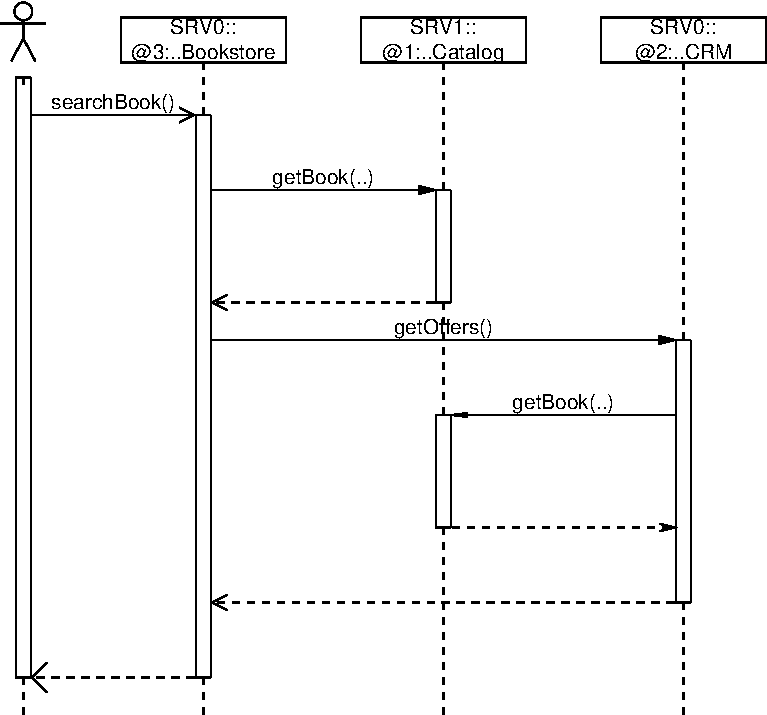
\includegraphics[scale=0.39]{\aspectJBookstoreApplicationDir/testdata/kieker-20100830-082225522-UTC-example-plots/deploymentSequenceDiagram-6488138950668976129-crop}
}
\subfigure[Trace \ldots{}6130]{\label{fig:appendix:traceAnalysisExample:SeqDiagrsDepl6130}%
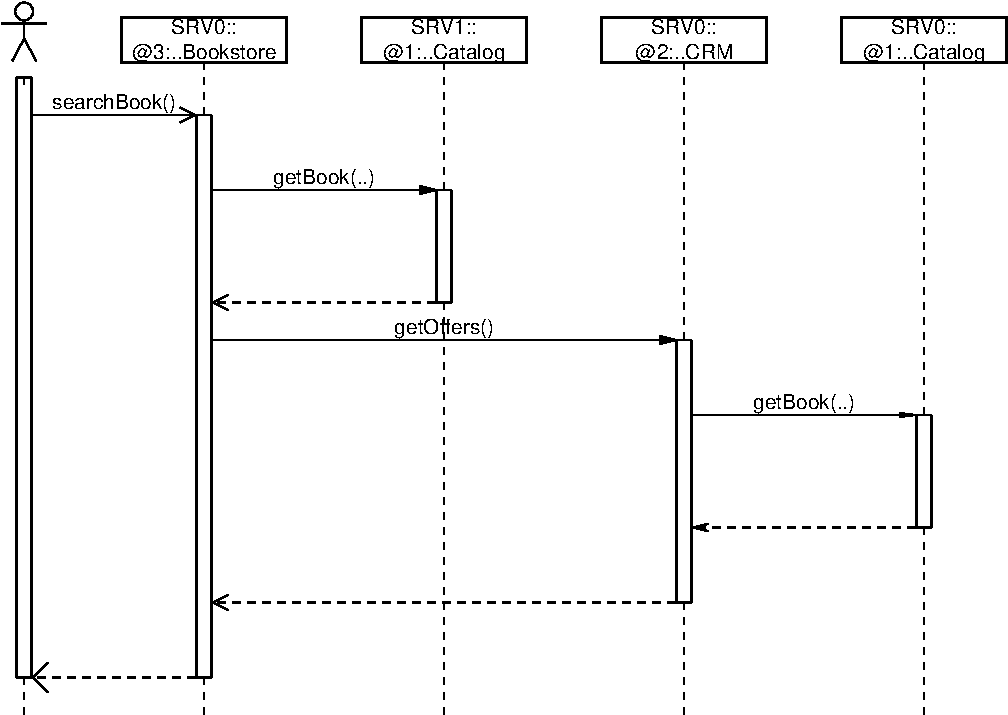
\includegraphics[scale=0.39]{\aspectJBookstoreApplicationDir/testdata/kieker-20100830-082225522-UTC-example-plots/deploymentSequenceDiagram-6488138950668976130-crop}
}
\subfigure[Trace \ldots{}6131]{\label{fig:appendix:traceAnalysisExample:SeqDiagrsDepl6131}%
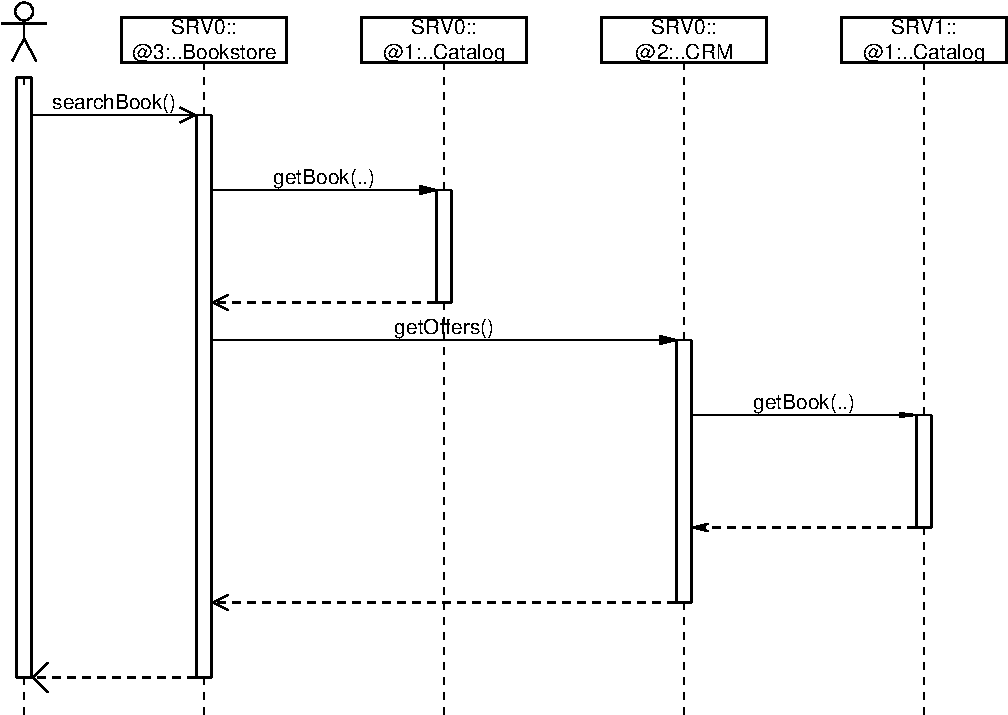
\includegraphics[scale=0.39]{\aspectJBookstoreApplicationDir/testdata/kieker-20100830-082225522-UTC-example-plots/deploymentSequenceDiagram-6488138950668976131-crop}
}
\subfigure[Trace \ldots{}6141]{\label{fig:appendix:traceAnalysisExample:SeqDiagrsDepl6141}%
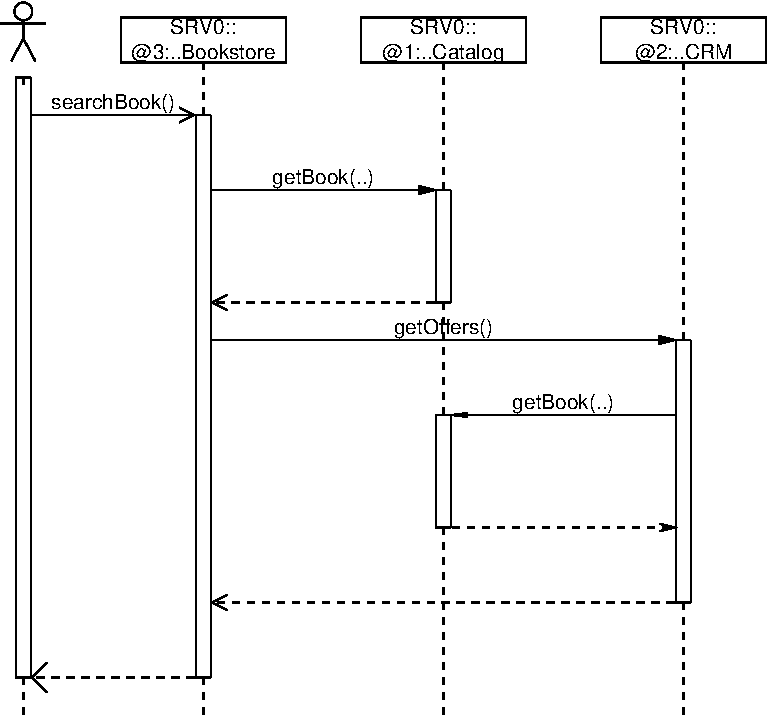
\includegraphics[scale=0.39]{\aspectJBookstoreApplicationDir/testdata/kieker-20100830-082225522-UTC-example-plots/deploymentSequenceDiagram-6488138950668976141-crop}
}
\caption{\textit{Deployment-level} sequence diagrams of the trace %
equivalence class representatives (Listing~\ref{lst:appendix:traceAnalysisExample:traceAssemblyEquivClasses})}
\label{fig:appendix:traceAnalysisExample:SeqDiagrsDepl}
\end{figure}

% \enlargethispage{2cm}
\pagebreak

\subsubsection{Assembly-Level Sequence Diagrams}\label{sec:example:assemblySeqDiagrams}%

Assembly-level sequence diagrams are generated using the command-line option \OPT{\OPTplotAssemblySequenceDiagrams}. %
Figure~\ref{fig:appendix:traceAnalysisExample:SeqDiagrDepl6129} %
shows the sequence diagram for the assembly-level trace equivalence representative %
(Section~\ref{sec:example:traceEquivClasses}).

\begin{figure}[h]\centering
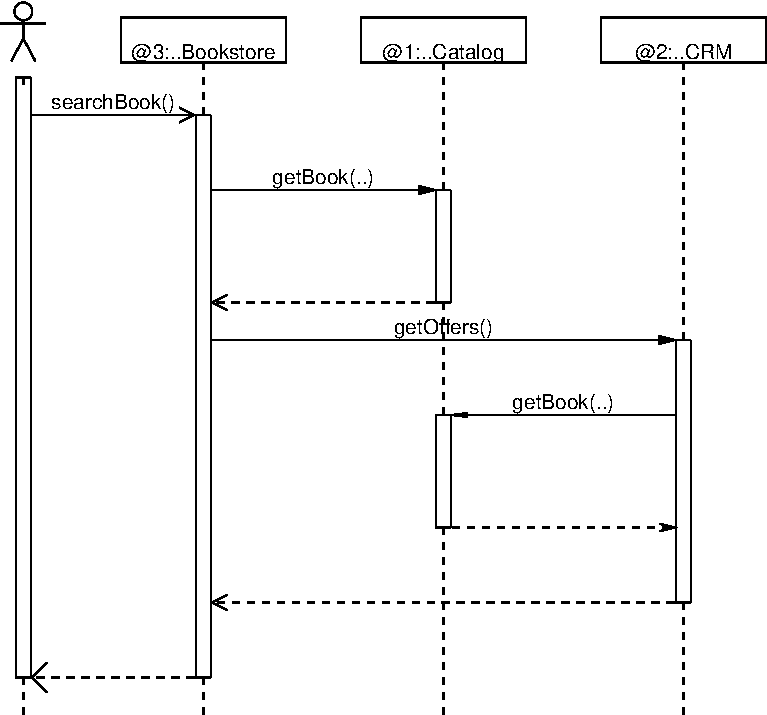
\includegraphics[scale=0.39]{\aspectJBookstoreApplicationDir/testdata/kieker-20100830-082225522-UTC-example-plots/assemblySequenceDiagram-6488138950668976129-crop}
\caption{\textit{Assembly-level} sequence diagram of trace \ldots{}6129}
\label{fig:appendix:traceAnalysisExample:SeqDiagrDepl6129}
\end{figure}

% \pagebreak

\subsection{Call Trees}\label{sec:example:callTrees}%

\subsubsection{Trace Call Trees}\label{sec:example:traceCallTrees}%

\enlargethispage{1.2cm}

Trace call trees are generated using the command-line option \OPT{\OPTplotCallTrees}. %
Figures~\ref{fig:appendix:traceAnalysisExample:TraceCallTrees6129}--\ref{fig:appendix:traceAnalysisExample:TraceCallTrees6141} %
show these call trees for each deployment-level %
trace equivalence representative (Section~\ref{sec:example:traceEquivClasses}).

\begin{figure}[h]\centering
\subfigure[Trace \ldots{}6129]{\label{fig:appendix:traceAnalysisExample:TraceCallTrees6129}%
\ \ 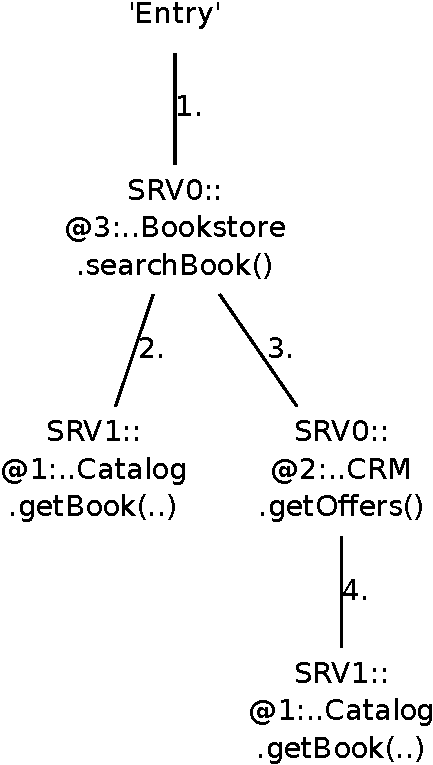
\includegraphics[scale=0.4]{\aspectJBookstoreApplicationDir/testdata/kieker-20100830-082225522-UTC-example-plots/callTree-6488138950668976129-crop}\ \ 
}
\subfigure[Trace \ldots{}6130]{\label{fig:appendix:traceAnalysisExample:TraceCallTrees6130}%
\ \ 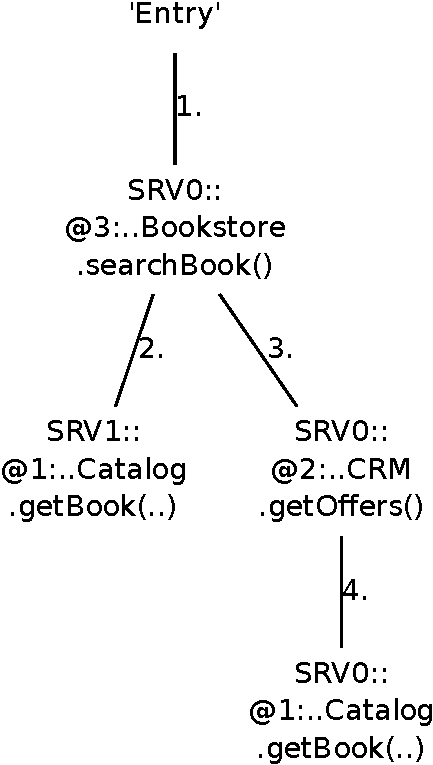
\includegraphics[scale=0.4]{\aspectJBookstoreApplicationDir/testdata/kieker-20100830-082225522-UTC-example-plots/callTree-6488138950668976130-crop}\ \ 
}
\subfigure[Trace \ldots{}6131]{\label{fig:appendix:traceAnalysisExample:TraceCallTrees6131}%
\ \ 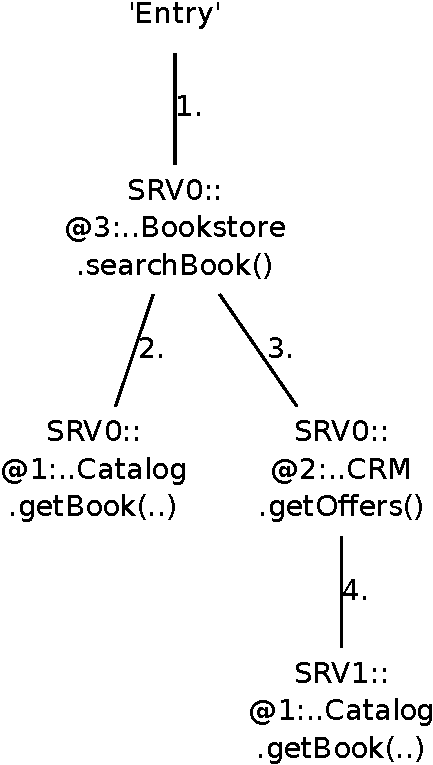
\includegraphics[scale=0.4]{\aspectJBookstoreApplicationDir/testdata/kieker-20100830-082225522-UTC-example-plots/callTree-6488138950668976131-crop}\ \ 
}
\subfigure[Trace \ldots{}6141]{\label{fig:appendix:traceAnalysisExample:TraceCallTrees6141}%
\ \ 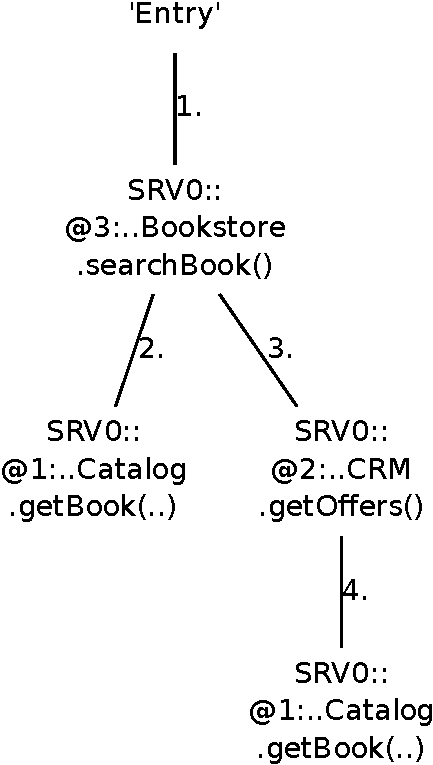
\includegraphics[scale=0.4]{\aspectJBookstoreApplicationDir/testdata/kieker-20100830-082225522-UTC-example-plots/callTree-6488138950668976141-crop}\ \ 
}
\caption{Calls trees of the trace %
equivalence class representatives (Listing~\ref{lst:appendix:traceAnalysisExample:traceAssemblyEquivClasses})}
\label{fig:appendix:traceAnalysisExample:TraceCallTrees}
\end{figure}

% \newpage

\subsubsection{Aggregated Call Trees}\label{sec:example:aggregatedCallTrees}%

Aggregated deployment/assembly-level call trees are generated using the command-line options %
\OPT{\OPTplotAggregatedDeploymentCallTree} and \OPT{\OPTplotAggregatedAssemblyCallTree}. %
Figures~\ref{fig:appendix:traceAnalysisExample:AggregatedCallTreesDeployment} and \ref{fig:appendix:traceAnalysisExample:AggregatedCallTreesAssembly} %
show these aggregated call trees for the traces contained in the monitoring data %
used in this section. %

\begin{figure}[h]\centering
\subfigure[deployment-level]{\label{fig:appendix:traceAnalysisExample:AggregatedCallTreesDeployment}%
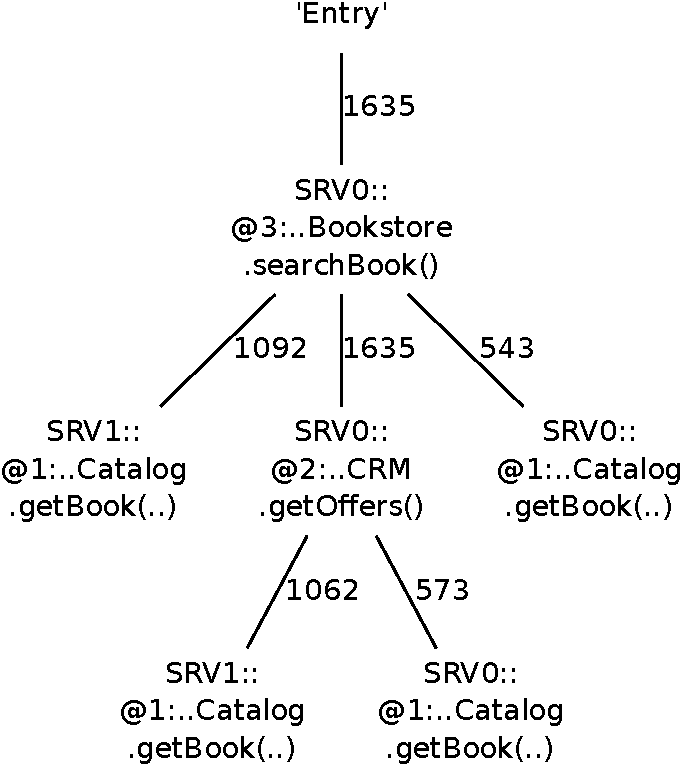
\includegraphics[scale=0.4]{\aspectJBookstoreApplicationDir/testdata/kieker-20100830-082225522-UTC-example-plots/aggregatedDeploymentCallTree-crop}%
}
\subfigure[assembly-level]{\label{fig:appendix:traceAnalysisExample:AggregatedCallTreesAssembly}%
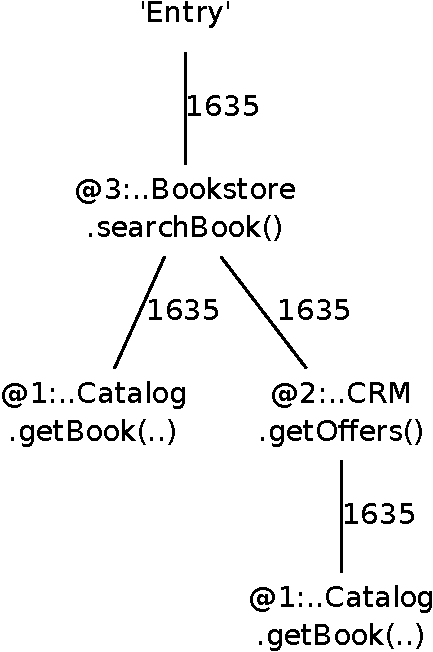
\includegraphics[scale=0.4]{\aspectJBookstoreApplicationDir/testdata/kieker-20100830-082225522-UTC-example-plots/aggregatedAssemblyCallTree-crop}%
}
\caption{Aggregated call trees generated from the 1635~traces}
\label{fig:appendix:traceAnalysisExample:AggregatedCallTrees}
\end{figure}

\pagebreak

\subsection{Dependency Graphs}

\subsubsection{Container Dependency Graphs}

A container dependency graph is generated using the command-line option %
\OPT{\OPTplotContainerDependencyGraph}. %
Figure~\ref{fig:appendix:traceAnalysisExample:ContainerDepGraph} shows the %
container dependency graph for the monitoring data used in this section. 

\begin{figure}[h]\centering
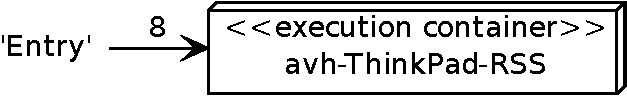
\includegraphics[scale=0.45]{\aspectJBookstoreApplicationDir/testdata/kieker-20100830-082225522-UTC-example-plots/containerDependencyGraph-crop}
\caption{Container dependency graph}
\label{fig:appendix:traceAnalysisExample:ContainerDepGraph}
\end{figure}

\subsubsection{Component Dependency Graphs}

Deployment/assembly-level component dependency graphs are generated using the %
command-line options \OPT{\OPTplotDeploymentComponentDependencyGraph} and %
\OPT{\OPTplotAssemblyComponentDependencyGraph}. %
Figures~\ref{fig:appendix:traceAnalysisExample:ComponentDepGraphsDeployment} and %
\ref{fig:appendix:traceAnalysisExample:ComponentDepGraphsAssembly} show the %
component dependency graphs for the monitoring data used in this section. 

\begin{figure}[h]\centering
\subfigure[deployment-level]{\label{fig:appendix:traceAnalysisExample:ComponentDepGraphsDeployment}%
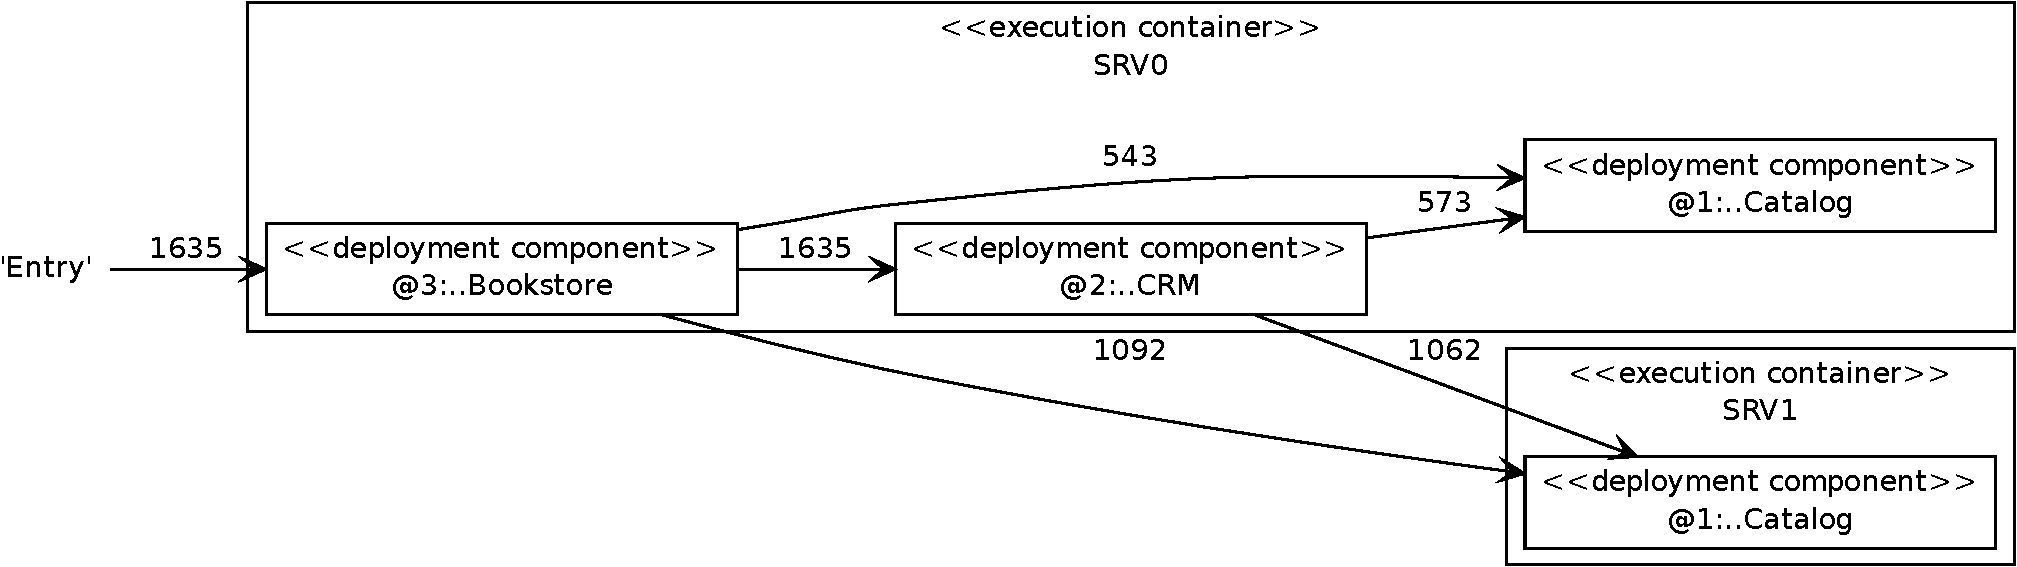
\includegraphics[scale=0.45]{\aspectJBookstoreApplicationDir/testdata/kieker-20100830-082225522-UTC-example-plots/deploymentComponentDependencyGraph-crop}
}
\subfigure[assembly-level]{\label{fig:appendix:traceAnalysisExample:ComponentDepGraphsAssembly}%
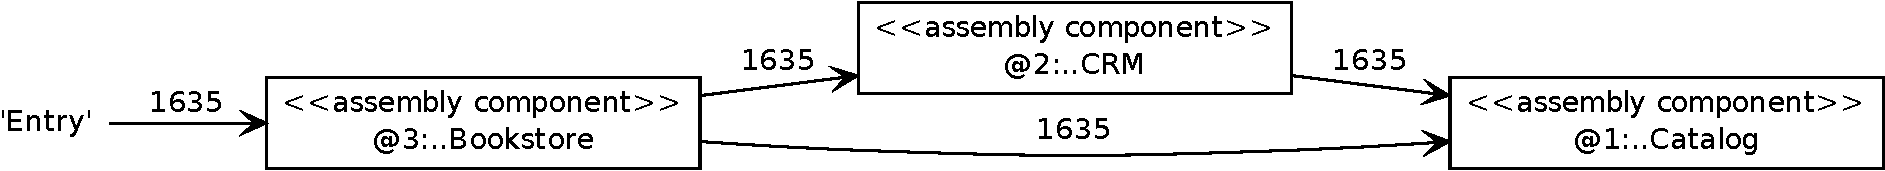
\includegraphics[scale=0.45]{\aspectJBookstoreApplicationDir/testdata/kieker-20100830-082225522-UTC-example-plots/assemblyComponentDependencyGraph-crop}
}
\caption{Component dependency graphs}
\label{fig:appendix:traceAnalysisExample:ComponentDepGraphs}
\end{figure}

\pagebreak

\subsubsection{Operation Dependency Graphs}

Deployment/assembly-level operation dependency graphs are generated using the %
command-line options \OPT{\OPTplotDeploymentOperationDependencyGraph} and %
\OPT{\OPTplotAssemblyOperationDependencyGraph}. %
Figures~\ref{fig:appendix:traceAnalysisExample:OperationDepGraphsDeployment} and %
\ref{fig:appendix:traceAnalysisExample:OperationDepGraphsAssembly} show the %
operation dependency graphs for the monitoring data used in this section. 

\begin{figure}[ht]\centering
\subfigure[deployment-level]{\label{fig:appendix:traceAnalysisExample:OperationDepGraphsDeployment}%
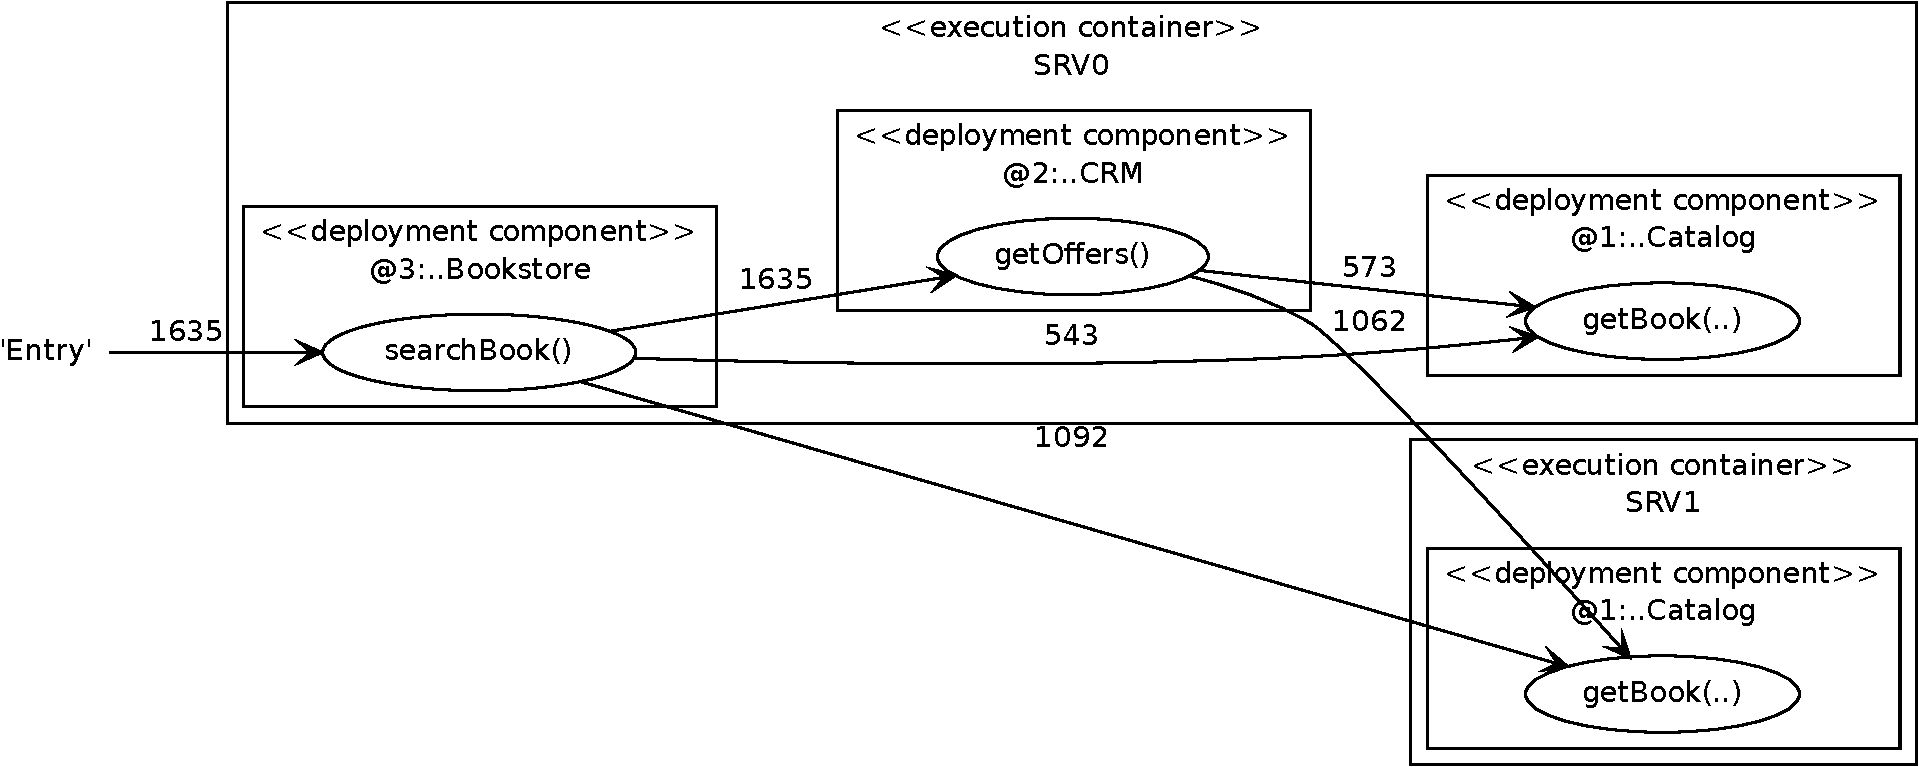
\includegraphics[scale=0.4]{\aspectJBookstoreApplicationDir/testdata/kieker-20100830-082225522-UTC-example-plots/deploymentOperationDependencyGraph-crop}
}
\subfigure[assembly-level]{\label{fig:appendix:traceAnalysisExample:OperationDepGraphsAssembly}%
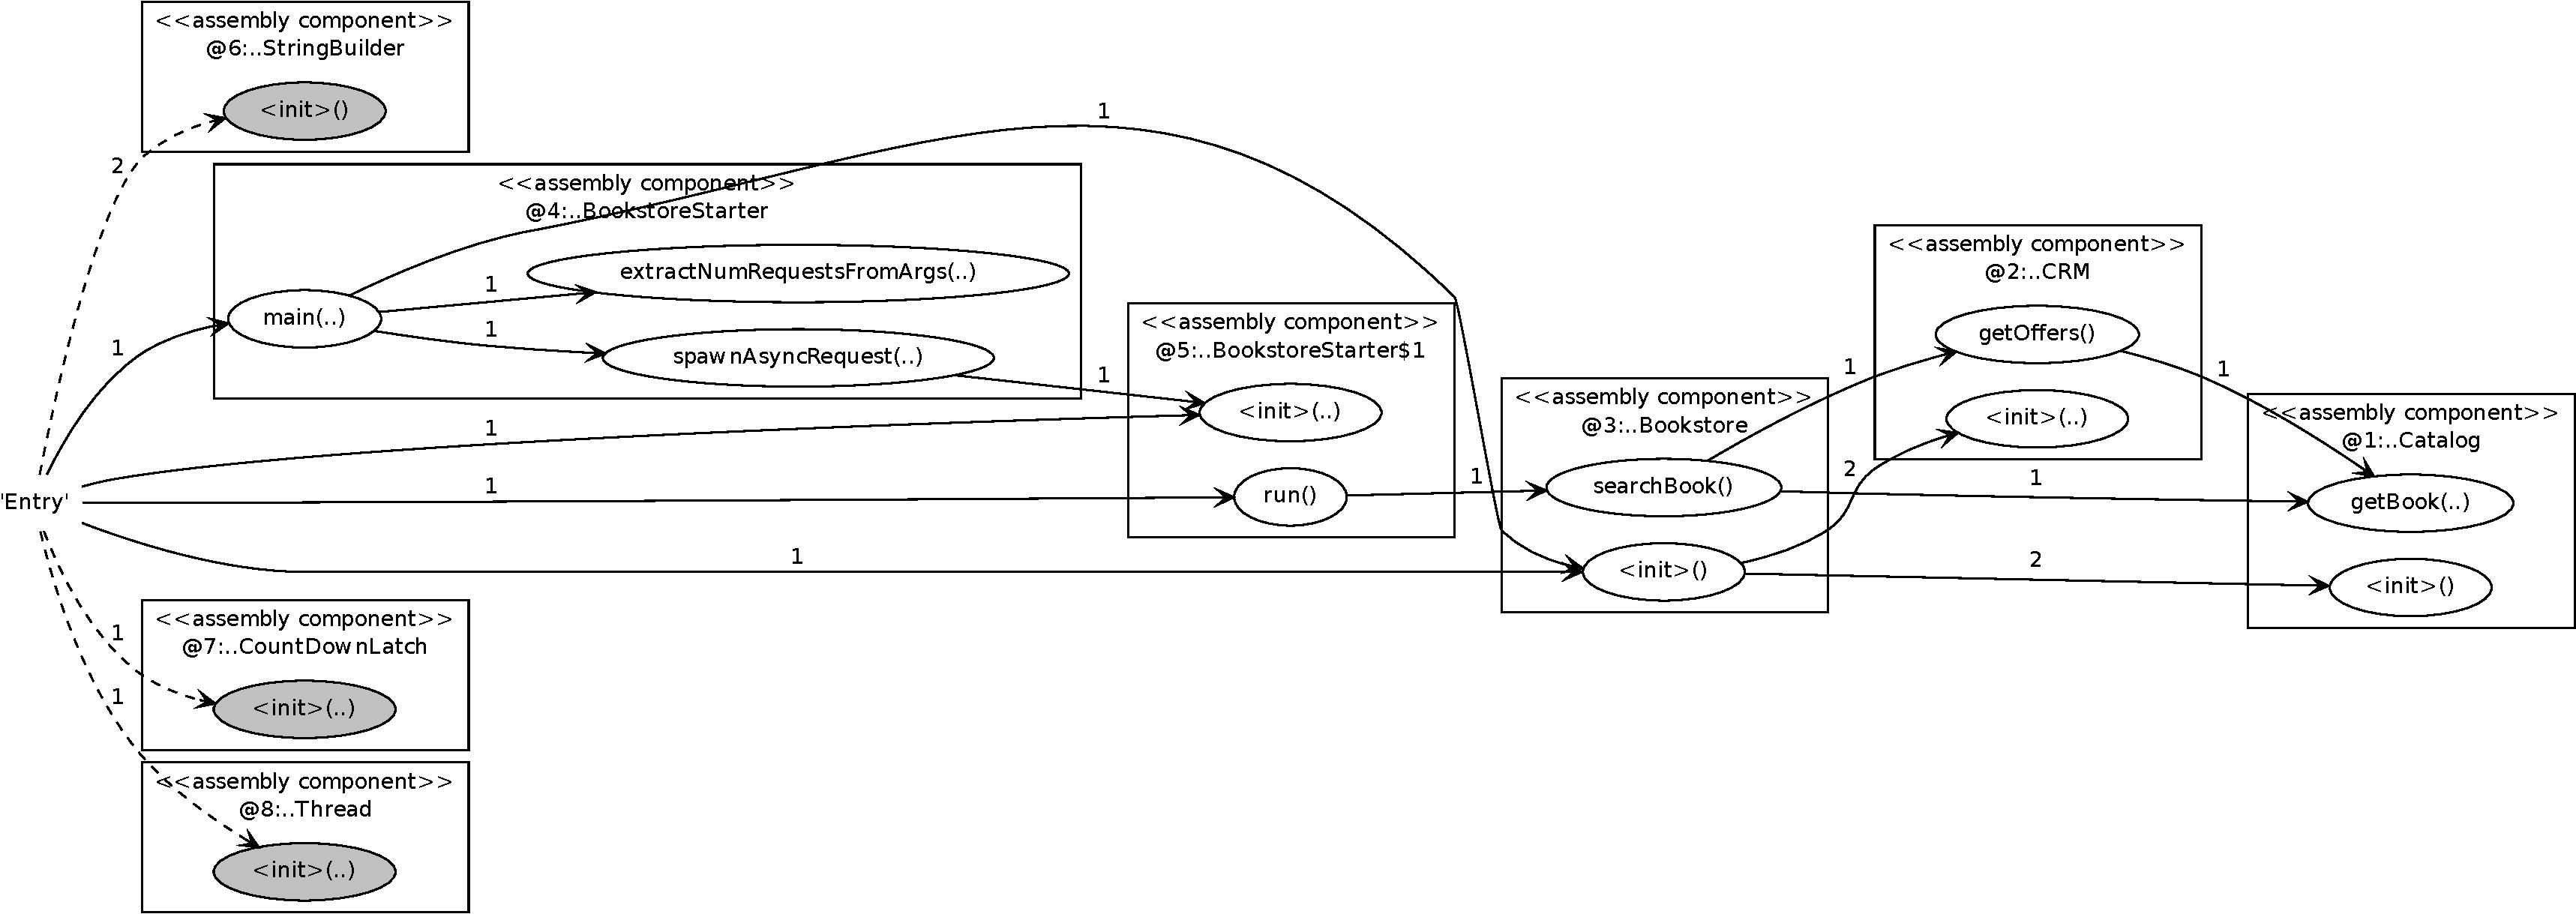
\includegraphics[scale=0.4]{\aspectJBookstoreApplicationDir/testdata/kieker-20100830-082225522-UTC-example-plots/assemblyOperationDependencyGraph-crop}
}
\caption{Operation dependency graphs}
\label{fig:appendix:traceAnalysisExample:OperationDepGraphs}
\end{figure}

% \pagebreak

\enlargethispage{1.5cm}

\subsection{Response Times in Dependency Graphs}

The afore-mentioned dependency graphs can also be decorated by the response times, adding the minimum, the average, %
and the maximum response times of the components. The decoration will be generated with one of the additional %
\OPT{responseTimes} command line parameters behind the corresponding \OPT{plot-}command.  %
An exemplaric graph with response times is shown in Figure~\ref{fig:appendix:traceAnalysisExample:graphWithRespTimes}.

\begin{figure}[h]
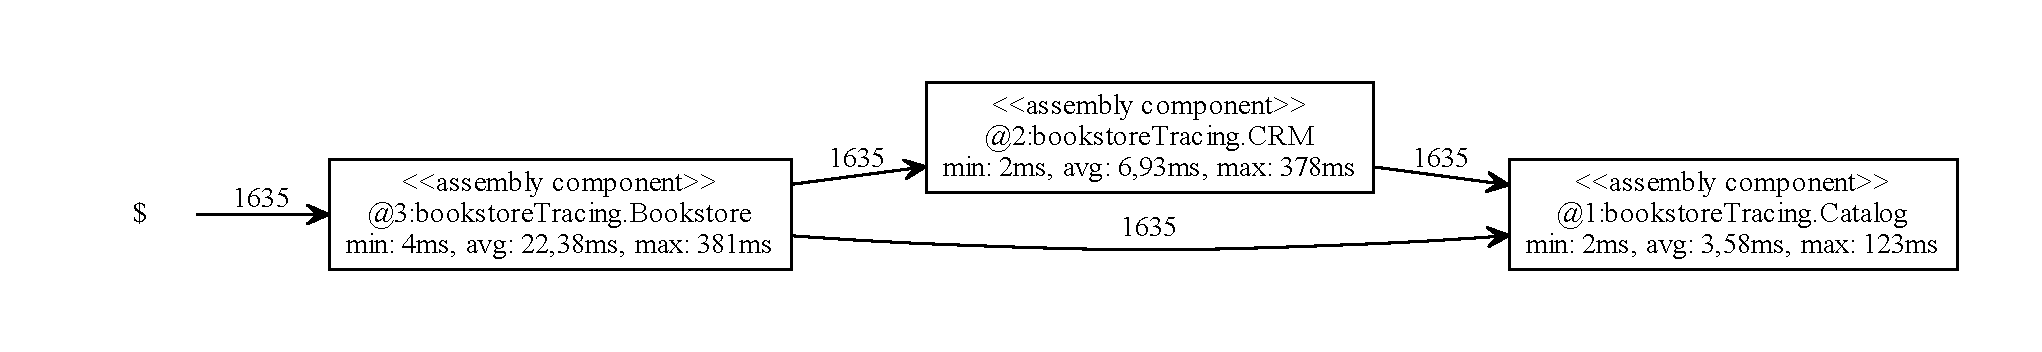
\includegraphics[scale=0.45]{images/assemblyComponentDependencyGraphWithResponseTimes}
\caption{Assembly component dependency graph with response times}
\label{fig:appendix:traceAnalysisExample:graphWithRespTimes}
\end{figure}
   

\pagebreak

\subsection{HTML Output of the System Model}

\KiekerTraceAnalysis{} writes an HTML representation of the system model reconstructed %
from the trace data to a file \file{system-entities.html}. %
Figure~\ref{fig:appendix:traceAnalysisExample:htmlSystemModel} shows a screenshot %
of this file rendered by a web browser.

\enlargethispage{1.5cm}

\begin{figure}[h!]\centering
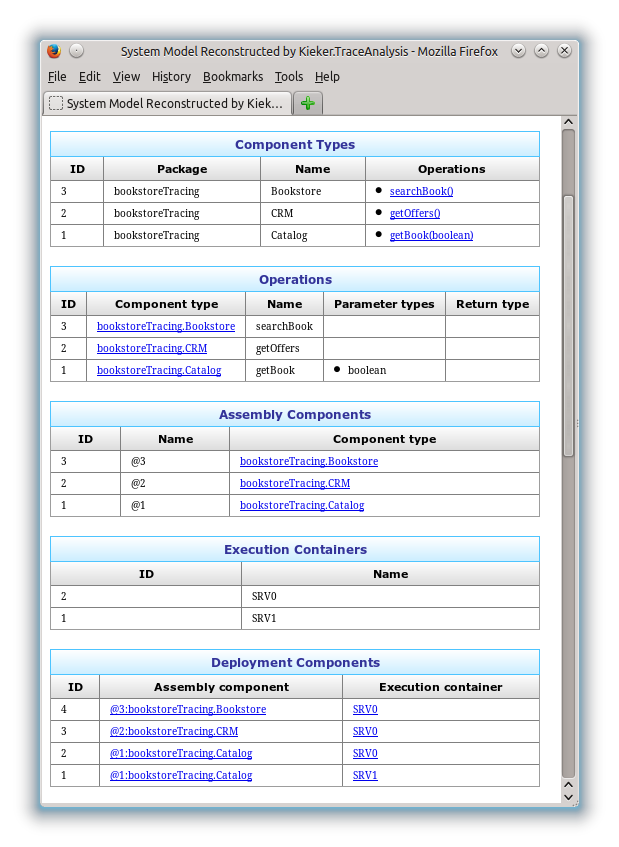
\includegraphics[width=0.75\textwidth]{images/system-entities-html-FFscrsh.png}
\caption{HTML output of the system model reconstructed from the traces}
\label{fig:appendix:traceAnalysisExample:htmlSystemModel}
\end{figure}



  %%%%%%%%%%%%%%%%%%%%%%%%%%%%%%%%%%%%%%%%%
% Appendix
% 
% $Date$
% $Rev$:
% $Author$

\newpage
\appendix

% \chapter*{Appendix}\label{appendix}
\phantomsection
\addtocontents{toc}{\protect\pagebreak}
\addcontentsline{toc}{chapter}{Appendix}\hypertarget{hypertarget:appendix}{}
\addtocontents{toc}{\protect\setcounter{tocdepth}{0}}

\chapter{Wrapper Scripts}\label{appendix:wrapperScripts}
The \dir{bin/} directory of \Kieker's binary release contains some \file{.sh}  and %
\file{.bat} scripts to invoke tools included in \file{\mainJar{}}. %
The following sections give a short description of their functionality and %
list their usage outputs as printed to the standard output stream when %
called without command-line parameters. %
In addition to the standard output stream, the file \file{kieker.log} %
is used for logging output during execution.

% generated by the script gen-bin-usage-tex.sh with manual adjustments

\

\WARNBOX{%
The Windows \file{.bat} wrapper scripts must be executed from within %
the \dir{bin/} directory.
}

\section{Script \file{convertLoggingTimestamp.sh|bat}}

The script converts \KiekerMonitoringPart{} logging timestamps, %
representing the number of nanoseconds since 1~Jan 1970 00:00 UTC, to a %
human-readable textual representation in the UTC and local timezones. %

\

\noindent Main-class: {\small \class{kieker.tools.loggingTimestampConverter.LoggingTimestampConverterTool}}

\paragraph*{Usage}\

\setTextListing
\lstinputlisting[caption=]{Appendix-usage-convertLoggingTimestamp.sh.inc}

\paragraph*{Example}\

The following listing shows the command to convert two logging timestamps as %
well as the resulting output.

\enlargethispage{0.7cm}

\setTextListing
\begin{lstlisting}[caption=Execution under UNIX-like systems]
$\lstshellprompt{}$ $\textbf{bin/convertLoggingTimestamp.sh}$ $\textbf{-\,-timestamps}$ 1283156545581511026 1283156546127117246 
1283156545581511026: Mo, 30 Aug 2010 08:22:25 +0000 (UTC) (Mo, 30 Aug 2010 10:22:25 +0200 (local time))
1283156546127117246: Mo, 30 Aug 2010 08:22:26 +0000 (UTC) (Mo, 30 Aug 2010 10:22:26 +0200 (local time))
\end{lstlisting}

\begin{lstlisting}[caption=Execution under Windows]
$\lstshellprompt{}$ $\textbf{convertLoggingTimestamp.bat}$ $\textbf{-\,-timestamps}$ 1283156545581511026 1283156546127117246 
1283156545581511026: Mo, 30 Aug 2010 08:22:25 +0000 (UTC) (Mo, 30 Aug 2010 10:22:25 +0200 (local time))
1283156546127117246: Mo, 30 Aug 2010 08:22:26 +0000 (UTC) (Mo, 30 Aug 2010 10:22:26 +0200 (local time))
\end{lstlisting}

% \pagebreak

\section{Script \file{logReplay.sh|bat}}

Replays filesystem monitoring logs created by \KiekerMonitoringPart{}. %
Example applications are:
\begin{compactitem}
\item Merging multiple directories containing monitoring data into a single %
output directory. 
\item Importing a filesystem monitoring log to another monitoring log, e.g., %
a database. Therefore, an appropriate \KiekerMonitoringPart{} configuration %
file must be passed to the script (see Section~\ref{sec:monitoring:configuration}).
\item Replaying a recorded filesystem monitoring log in real-time (or faster/slower) in order to simulate %
incoming monitoring data from a running system, e.g., via JMS~(see also Appendix~\ref{appendix:usingJMS}). 
\end{compactitem}

\

\noindent Main-class: {\small \class{kieker.tools.logReplayer.FilesystemLogReplayerStarter}}

\paragraph*{Usage}\

\setTextListing
\lstinputlisting[caption=]{Appendix-usage-logReplay.sh.inc}

\paragraph*{Example}\

\noindent The following command replays the monitoring testdata included in %
the binary release to another directory:

% \pagebreak

\setTextListing
\begin{lstlisting}[caption=Execution under UNIX-like systems]
$\lstshellprompt{}$ $\textbf{bin/logReplay.sh}$
  $\textbf{-\,-inputdirs}$ $\distributedTestdataReleaseDirDistro$ 
  $\textbf{-\,-keep-logging-timestamps}$ $true$ 
  $\textbf{-\,-realtime}$ $false$
\end{lstlisting}
\begin{lstlisting}[caption=Execution under Windows]
$\lstshellprompt{}$ $\textbf{logReplay.bat}$
  $\textbf{-\,-inputdirs}$ $\distributedTestdataReleaseDirDistroWin$ 
  $\textbf{-\,-keep-logging-timestamps}$ $true$ 
  $\textbf{-\,-realtime}$ $false$
\end{lstlisting}


\section{Script \file{kax-run.sh|bat}}\label{appendix:wrapperScripts:kaxRun}

Executes a \KiekerAnalysisPart{} pipe-and-filter configuration file (\file{.kax} file), %
described in Section~\ref{sec:analysis:controller}. %

\noindent Main-class: {\small \class{kieker.tools.KaxRun}}

\paragraph*{Usage}\

\setTextListing
\lstinputlisting[caption=]{Appendix-usage-kax-run.sh.inc}

\section{Script \file{kax-viz.sh|bat}}\label{appendix:wrapperScripts:kaxViz}

Visualizes a \KiekerAnalysisPart{} pipe-and-filter configuration file (\file{.kax} file), %
described in Section~\ref{sec:analysis:controller}. %

\noindent Main-class: {\small \class{kieker.tools.KaxViz}}

\paragraph*{Usage}\

\setTextListing
\lstinputlisting[caption=]{Appendix-usage-kax-viz.sh.inc}

\section{Script \file{trace-analysis.sh|bat}}\label{appendix:wrapperScripts:traceAnalysis}

Calls \KiekerTraceAnalysis{} to analyze and visualize monitored trace data, %
as described in Chapter~\ref{chap:aspectJ}.

\

\noindent Main-class: {\small \class{kieker.tools.traceAnalysis.TraceAnalysisTool}}

% \pagebreak

\paragraph*{Usage}\

\enlargethispage{1cm}

\setTextListing
\lstinputlisting[caption=]{Appendix-usage-trace-analysis.sh.inc}

\paragraph*{Example}\

\noindent The following commands generate a deployment-level operation dependency 
graph and convert it to pdf format:

\enlargethispage{1cm}

\setTextListing
\begin{lstlisting}[caption=Execution under UNIX-like systems]
$\lstshellprompt{}$ $\textbf{bin/trace-analysis.sh}$
  $\textbf{-\,-inputdirs}$ $\distributedTestdataReleaseDirDistro$ 
  $\textbf{-\,-outputdir}$ . 
  $\textbf{-\,-plot-Deployment-Operation-Dependency-Graph}$
$\lstshellprompt{}$ $\textbf{dot}$ $\textbf{-T}$ pdf  deploymentOperationDependencyGraph.dot > deploymentOperationDependencyGraph.pdf
\end{lstlisting}

\begin{lstlisting}[caption=Execution under Windows]
$\lstshellprompt{}$ $\textbf{trace-analysis.bat}$
  $\textbf{-\,-inputdirs}$ $\distributedTestdataReleaseDirDistroWin$ 
  $\textbf{-\,-outputdir}$ . 
  $\textbf{-\,-plot-Deployment-Operation-Dependency-Graph}$
$\lstshellprompt{}$ $\textbf{dot}$ $\textbf{-T}$ pdf  deploymentOperationDependencyGraph.dot > deploymentOperationDependencyGraph.pdf
\end{lstlisting}

\noindent Additional examples can be found in Chapter~\ref{chap:aspectJ}.

\section{Script \file{dotPic-fileConverter.sh|bat}}\label{appendix:wrapperScripts:dotPicFileConverter}

Converts each \file{.dot} and \file{.pic} file, e.g., diagrams generated by %
\KiekerTraceAnalysis{} (Section~\ref{chap:aspectJ}), located in a directory %
into desired graphic output formats. %
This scripts simply calls the \textit{Graphviz} and \textit{PlotUtils} tools \file{dot} and \file{pic2plot}.

\paragraph*{Usage}\

\setTextListing
\lstinputlisting[caption=,firstline=3,lastline=3]{Appendix-usage-dotPic-fileConverter.sh.inc}

\paragraph*{Example}\

\noindent The following command converts each \file{.dot} and \file{.pic} file located in the %
directory \dir{out/} to files in \file{.pdf} and \file{.png} format:

\setTextListing
\begin{lstlisting}[caption=Execution under UNIX-like systems]
$\lstshellprompt{}$ $\textbf{bin/dotPic-fileConverter.sh}$ out/ pdf png
\end{lstlisting}
\begin{lstlisting}[caption=Execution under Windows]
$\lstshellprompt{}$ $\textbf{dotPic-fileConverter.bat}$ out\ pdf png
\end{lstlisting}

\chapter{Java~EE Servlet Container Example}\label{appendix:JavaEEServletExample}
Using the sample Java web application %
MyBatis JPetStore,\footnote{\url{http://www.mybatis.org/spring/sample.html}} this example %
demonstrates how to employ \KiekerMonitoringPart{} for monitoring a Java application %
running in a Java~EE container---in this case Jetty.\footnote{\url{http://www.eclipse.org/jetty/}} %
Monitoring probes based on the Java~EE Servlet API, Spring, %
and AspectJ are used to monitor execution, trace, and session data (see Section~\ref{chap:aspectJ}). %
The directory \dir{\JavaEEServletExampleReleaseDirDistro/} contains the prepared Jetty %
server with the MyBatis JPetStore application and the \Kieker-based demo %
analysis application known from \url{http://demo.kieker-monitoring.net/}. %

\section{Setting}

The subdirectory \file{jetty/} includes the %
Jetty server with the JPetStore application already deployed to the server's %
\file{webapps/} directory. The example is prepared to use two alternative %
types of \Kieker{} probes: either the \Kieker{} Spring interceptor (default) or the 
\Kieker{} AspectJ aspects. Both alternatives additionally use \Kieker{}'s Servlet 
filter. %

\paragraph{Required Libraries and \KiekerMonitoringPart{} Configuration}

Both settings require the files \file{\aspectJWeaverJar{}} and \file{\mainJar}, %
which are already included in the webapps's \dir{WEB-INF/lib/} directory. %
Also, a \Kieker{} configuration file is already included in the Jetty's root directory, %
where it is considered for configuration by \KiekerMonitoringPart{} in both modes. 

\paragraph{Servlet Filter (Default)}

The file \file{web.xml} is located in the webapps's %
\dir{WEB-INF/} directory. \Kieker{}'s Servlet filters are already enabled: 

\setXMLListing
\lstinputlisting[firstline=50,lastline=61, numbers=none, linewidth=1\textwidth, caption=Enabling the Servlet filter in \file{web.xml}]{\JavaEEServletExampleDir/jetty/webapps/jpetstore/WEB-INF/web.xml}

\noindent This filter can be used with both the Spring-based and the %
AspectJ-based instrumentation mode.

\paragraph{Spring-based Instrumentation (Default)}

\Kieker{}'s Spring interceptor are already enabled in the file 
\file{applicationContext.xml}, located in the webapps's \dir{WEB-INF/} directory: 

\setXMLListing
\lstinputlisting[firstline=38,lastline=43, numbers=none, linewidth=1\textwidth, caption=Enabling the Spring interceptor in \file{applicationContext.xml}]{\JavaEEServletExampleDir/jetty/webapps/jpetstore/WEB-INF/applicationContext.xml}

\NOTIFYBOX{When using, for example, the \texttt{@Autowired} feature in your Spring beans, it can be necessary to force the usage of CGLIB proxy objects with \texttt{<aop:aspectj-autoproxy proxy-target-class="true"/>}.}

\paragraph{AspectJ-based Instrumentation}

\enlargethispage{1cm}

In order to use AspectJ-based instrumentation, the following changes need to 
be performed. The file \file{start.ini}, located in Jetty's root directory, %
allows to pass various JVM arguments, JVM system properties, and other options %
to the server on startup. When using AspectJ for instrumentation, the respective %
JVM argument needs to be activated in this file. %

The AspectJ configuration file \file{aop.xml} is already located in the %
webapps's\linebreak \dir{WEB-INF/classes/META-INF/} directory and configured to instrument %
the JPetStore classes with \Kieker{}'s \class{OperationExecutionAspectFull} aspect %
(Section~\ref{chap:aspectJ}). 

\

When using the AspectJ-based instrumentation, make sure to disable the Spring %
interceptor in the file \file{applicationContext.xml}, mentioned above. %

\begin{compactenum}
\item Start the Jetty server using the \file{start.jar} file (e.g., via \texttt{java -jar start.jar}). You should make %
   sure that the server started properly by taking a look at %
   the console output that appears during server startup.  
\item Now, you can access the JPetStore application by opening the URL
   \url{http://localhost:8080/jpetstore/} (Figure~\ref{fig:jpetstore}). %
   \Kieker{} initialization messages should appear in the console output. %
   
\begin{figure}[h]\centering
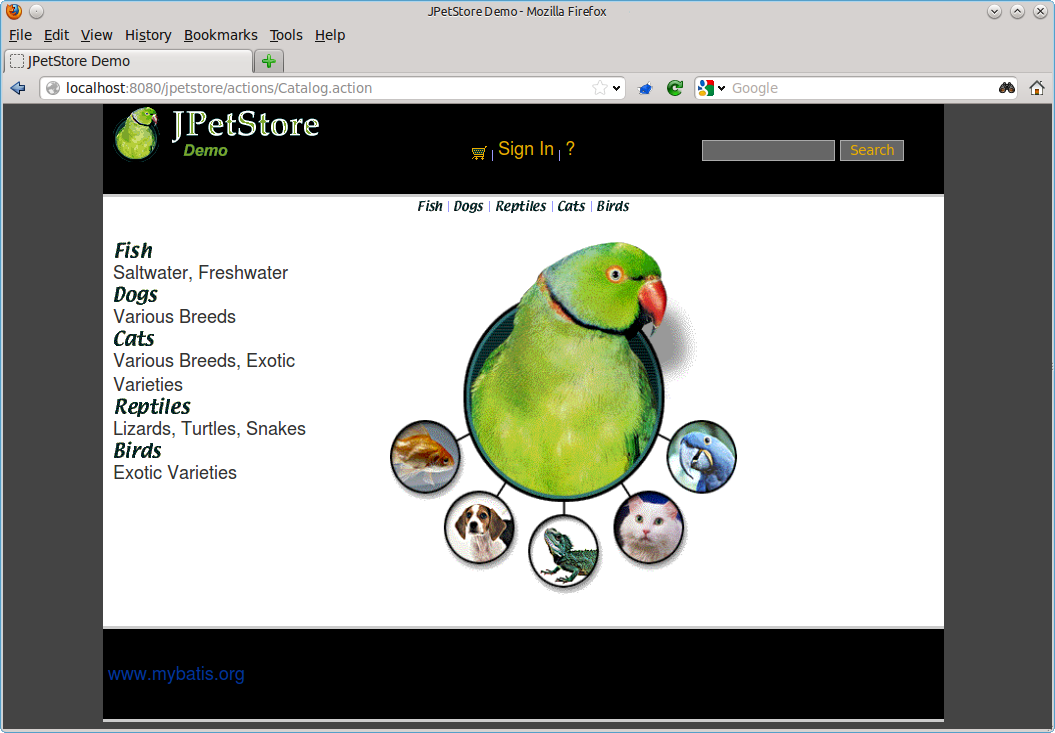
\includegraphics[width=0.8\textwidth]{images/jpetstore-example-FFscrsh}
\caption{MyBatis JPetStore}\label{fig:jpetstore}%
\end{figure}
   
\item   Browse through the application to generate some monitoring data. %
\item In this example, \Kieker{} is configured to write the monitoring data %
      to JMX in order to communicate with the \Kieker-based demo analysis %
      application, which is accessible via \url{localhost:8080/livedemo/}.
   
\item In order to write the monitoring data to the file system, the %
      JMX writer needs to be disabled in the file \file{kieker.monitoring.properties}, %
      which is located in the directory \file{webapps/jpetstore/WEB-INF/classes/META-INF/}.
      After a restart of the Jetty server, the Kieker startup output includes the %
      information where the monitoring data is written to (should be a %
      \dir{kieker-<DATE-TIME>/} directory) located in the default temporary %
      directory. %
   This data can be analyzed and visualized using \KiekerTraceAnalysis{}, %
   as described in Chapter~\ref{chap:aspectJ}.
\end{compactenum}

\medskip

 

\chapter{Using the JMS Writer and Reader}\label{appendix:usingJMS}
This chapter gives a brief description on how to use the \class{AsyncJmsWriter} and \class{JmsReader} %
classes. The directory \dir{\JMSBookstoreApplicationReleaseDirDistro/} contains the %
sources, gradle scripts etc.\ used in this example. It is based on the Bookstore %
application with manual instrumentation presented in Chapter~\ref{chap:example}. %

The following sections provide step-by-step instructions for the %
ActiveMQ JMS server implementation (Section~\ref{example:jms:activemq}).
The general procedure for this example is the following:

\medskip

\begin{compactenum}
 \item Download and prepare the respective JMS server implementation
 \item Copy required libraries to the example directory
 \item Start the JMS server
 \item Start the analysis instance which receives records via JMS
 \item Start the monitoring instance which sends records via JMS
\end{compactenum}

\

\WARNBOX{\quad\\Due to a bug in some JMS servers, avoid paths including white spaces.}

\section{ActiveMQ}\label{example:jms:activemq}

\subsection{Download and Prepare ActiveMQ}

Download an ActiveMQ archive from \url{http://activemq.apache.org/download.html}
and decompress it to the base directory of the example. Note, that there are two different %
distributions, one for Unix/Linux/Cygwin and another one for Windows, and that the latest supported version of ActiveMQ compatible with Java 7 is 5.14.5. 

Under \UnixLikeSystems{}, you'll need to set the executable-bit of the start script:

\setBashListing
\begin{lstlisting}[caption=]
 #\lstshellprompt{}# chmod +x bin/activemq
\end{lstlisting}

\noindent Also under \UnixLikeSystems{}, make sure that the file \file{bin/activemq} %
includes UNIX line endings (e.g., using your favorite editor or the \textit{dos2unix} tool).

\subsection{Copy ActiveMQ Libraries}

Copy the following files from the ActiveMQ release to the %
\dir{lib/} directory of this example:

\medskip

\enlargethispage{0.5cm}

\begin{compactenum}
\item \file{activemq-all-<version>.jar} (from ActiveMQ's base directory)
\item \file{slf4j-log4j<version>.jar} (from ActiveMQ's \dir{lib/optional} directory)
\item \file{log4j-<version>.jar} (from ActiveMQ's \dir{lib/optional} directory)
\end{compactenum}

\subsection{Kieker Monitoring Configuration for ActiveMQ}

The file \file{src-resources/META-INF/kieker.\-monitoring.\-pro\-perties-activeMQ} %
is already configured to use the \class{JmsWriter} via ActiveMQ. The important properties are %
the definition of the provider URL and the context factory:

\setPropertiesListing
\lstinputlisting[firstline=12,lastline=12,caption=Excerpt from \file{kieker.monitoring.properties-activemq} configuring the provider URL of the JMS writer via ActiveMQ]{\JMSBookstoreApplicationDir/src-resources/META-INF/kieker.monitoring.properties-activemq}

\setPropertiesListing
\lstinputlisting[firstline=21,lastline=21,caption=Excerpt from \file{kieker.monitoring.properties-activemq} configuring the context factory of the JMS writer via ActiveMQ]{\JMSBookstoreApplicationDir/src-resources/META-INF/kieker.monitoring.properties-activemq}

\subsection{Running the Example}

% \paragraph*{Execution}%
 The execution of the example is performed by the following three steps:
\begin{enumerate}
\item Start the JMS server (you may have to set your \class{JAVA\_HOME} variable first):

\setBashListing
\begin{lstlisting}[caption=Start of the JMS server under UNIX-like systems]
#\lstshellprompt{}# bin/activemq start
\end{lstlisting}
\begin{lstlisting}[caption=Start of the JMS server under Windows]
#\lstshellprompt{}# bin\#activemq start
\end{lstlisting}
\item Start the analysis part (in a new terminal):
\setBashListing
\begin{lstlisting}[caption=Start the analysis part under UNIX-like systems]
#\lstshellprompt{}# ./gradlew runAnalysisActiveMQ
\end{lstlisting}
\begin{lstlisting}[caption=Start the analysis part under Windows]
#\lstshellprompt{}# gradlew.bat runAnalysisActiveMQ
\end{lstlisting}
\item Start the instrumented Bookstore (in a new terminal):
\setBashListing
\begin{lstlisting}[caption=Start the analysis part under UNIX-like systems]
#\lstshellprompt{}# ./gradlew runMonitoringActiveMQ
\end{lstlisting}
\begin{lstlisting}[caption=Start the analysis part under Windows]
#\lstshellprompt{}# gradlew.bat runMonitoringActiveMQ
\end{lstlisting}
\end{enumerate}


\chapter{Using the AMQP Writer and Reader}\label{appendix:usingAMQP}
This chapter gives a brief description on how to use the \class{AmqpWriter} and \class{AmqpReader} %
classes, which allow to use Kieker with AMQP-based queue implementations such as %
RabbitMQ.\footnote{\url{http://www.rabbitmq.com}} The directory \dir{\AMQPBookstoreApplicationReleaseDirDistro/} %
contains the sources, gradle scripts etc.\ used in this example. It is based on the Bookstore %
application with manual instrumentation presented in Chapter~\ref{chap:example}. %

The following paragraphs provide step-by-step instructions for the popular AMQP implementation RabbitMQ.%

\section{Preparation}

\subsection{Download and Install RabbitMQ}
Download the RabbitMQ distribution from \url{http://www.rabbitmq.com/download.html} and follow the installation %
instructions for your OS. Since RabbitMQ requires Erlang, additional software packages may have to be installed %
on your machine.
\par In order to use RabbitMQ's integrated management UI, you may have to enable the appropriate plugin first. This is %
done by issuing the following command from the command line. 

\setBashListing
\begin{lstlisting}[caption=Enable the management UI under UNIX-like systems]
#\lstshellprompt{}# rabbitmq-plugins enable rabbitmq_management
\end{lstlisting}
\begin{lstlisting}[caption=Enable the management UI under Windows]
#\lstshellprompt{}# rabbitmq-plugins enable rabbitmq_management
\end{lstlisting}

Once the UI is enabled, you may access it at port 15672 by default. %

\subsection{Configure RabbitMQ}
Once the RabbitMQ server is installed and started, create a queue for Kieker to use. This can be done easily using %
RabbitMQ's management UI. It is accessible via \url{http://localhost:15672} (the default credentials are \texttt{guest:guest}) We will assume a queue named \parameterValue{kieker} for the remainder of this %
example. Please note the following caveats when configuring the server:

\begin{compactenum}
 \item If you choose to create a transient queue, the entire queue (not just the queued messages) is destroyed %
 on server shutdown and must be re-created manually. %
 \item The RabbitMQ server's default permissions grant access only from \hostname{localhost}. If your RabbitMQ server runs %
 on a remote machine, you have to set the permissions accordingly. %
\end{compactenum}

\subsection{Kieker Monitoring Configuration for RabbitMQ}
The file \file{src-resources/META-INF/kieker.\-monitoring.\-pro\-perties} %
is already configured to use the \class{AMQPWriter}. The important properties are %
the server URI and the queue name. %

\setPropertiesListing
\lstinputlisting[firstline=9,lastline=9,caption=Excerpt from \file{kieker.monitoring.properties} configuring the URI of the AMQP server]{\AMQPBookstoreApplicationDir/src-resources/META-INF/kieker.monitoring.properties}

\setPropertiesListing
\lstinputlisting[firstline=15,lastline=15,caption=Excerpt from \file{kieker.monitoring.properties} configuring the AMQP queue name]{\AMQPBookstoreApplicationDir/src-resources/META-INF/kieker.monitoring.properties}

\section{Running the Example}
The execution of the example is performed by the following three steps:
\begin{enumerate}
\item Ensure that the RabbitMQ server is started and the configured queue is accessible.

\item Start the analysis part (in a new terminal):
\setBashListing
\begin{lstlisting}[caption=Start the analysis part under UNIX-like systems]
#\lstshellprompt{}# ./gradlew runAnalysisAMQP
\end{lstlisting}
\begin{lstlisting}[caption=Start the analysis part under Windows]
#\lstshellprompt{}# gradlew.bat runAnalysisAMQP
\end{lstlisting}
\item Start the instrumented Bookstore (in a new terminal):
\setBashListing
\begin{lstlisting}[caption=Start the analysis part under UNIX-like systems]
#\lstshellprompt{}# ./gradlew runMonitoringAMQP
\end{lstlisting}
\begin{lstlisting}[caption=Start the analysis part under Windows]
#\lstshellprompt{}# gradlew.bat runMonitoringAMQP
\end{lstlisting}
\end{enumerate}

\chapter{Sigar-Based Samplers for System-Level Monitoring}\label{appendix:SigarBasedSamplers}
This chapter gives a brief description on how to use the included %
periodic samplers (Section~\ref{sec:componentsMonitoring:monitoringController:periodicSamplers}) %
for monitoring CPU utilization and memory/swap usage. %
The directory \dir{\SigarExampleReleaseDirDistro/} contains the %
sources, gradle scripts etc.\ used in this example. %
These samplers employ the Sigar API~\cite{HypericSigarWebsite}. \\%

\section{Preparation}

\begin{compactenum}
\item Copy the files \file{\mainJarEMF} and \file{\sigarJar} from the %
binary distribution to the example's \dir{lib/} directory.
\item Additionally, depending on the underlying system platform, %
corresponding Sigar native libraries need to be placed in the example's \dir{lib/} directory. %
Kieker's \dir{lib/sigar-native-libs/} folder already includes the right libraries for 32 and 64~bit Linux/Windows platforms. %
Native libraries for other platforms can be downloaded from~\cite{HypericSigarWebsite}. %
\end{compactenum}

\section{Using the Sigar-Based Samplers}

\WARNBOX{
	Using a very short sampling period with Sigar ($< 500$ ms) can result in monitoring log entries with NaN values. 
}

The Sigar API~\cite{HypericSigarWebsite} provides access to a number of system-level inventory and monitoring data, %
e.g., regarding memory, swap, cpu, file system, and network devices. %
Kieker includes Sigar-based samplers %
for monitoring CPU utilization %
(\class{CPUsDetailedPercSampler}, \class{CPUsCombinedPercSampler}) %
and memory/swap usage (\class{MemSwapUsageSampler}). %
When registered as a periodic sampler (Section~\ref{sec:componentsMonitoring:monitoringController:periodicSamplers}), %
these samplers collect the data of interest employing the Sigar API, %
and write monitoring records of types \class{CPUUtilizationRecord}, %
\class{ResourceUtilizationRecord}, and \class{MemSwapUsageRecord} respectively %
to the configured monitoring log/stream. %

Listing~\ref{listing:sigarSamplerMonitoringStarterExample} shows an excerpt from %
this example's \class{MonitoringStarter} %
which creates and registers two Sigar-based peridioc samplers. %
For reasons of performance and thread-safety, the \class{SigarSamplerFactory} %
should be used to create instances of the Sigar-based Samplers. 

%\pagebreak

\setJavaCodeListing
\lstinputlisting[firstline=38, lastline=51, firstnumber=38, caption=Excerpt from MonitoringStarter.java, label=listing:sigarSamplerMonitoringStarterExample]{\SigarExampleDir/src/kieker/examples/userguide/appendixSigar/MonitoringStarter.java}

\noindent Based on the existing samplers, users can easily create custom Sigar-based %
samplers by extending the class \class{AbstractSigarSampler}. For example, Listing~%
\ref{listing:sigarSamplerMethod} in Section~\ref{sec:componentsMonitoring:monitoringController:periodicSamplers} %
shows the \class{MemSwapUsageSampler}'s \method{sample} method. %
Typically, it is also required to define a corresponding monitoring record type, %
as explained in Section~\ref{sec:componentsMonitoring:monitoringRecords}. %
When implementing custom Sigar-based samplers, the \class{SigarSamplerFactory}'s \method{getSigar} method should %
be used to retrieve a \class{Sigar} instance. %

This example uses a stand-alone Java application to set up %
a Sigar-based monitoring process. When using servlet containers,  %
users may consider implementing this routine as a \class{ServletContextListener}, %
which are executed when the container is started and shutdown. %
As an example, Kieker includes a \class{CPUMemUsageServletContextListener}. %

\section{Executing the Example}

The execution of the example is performed by the following two steps:\\

\begin{compactenum}
\item Monitoring CPU utilization and memory usage for 30~seconds (class \class{MonitoringStarter}):
\setBashListing
\begin{lstlisting}[caption=Start of the monitoring under UNIX-like systems]
#\lstshellprompt{}# #\textbf{./gradlew}# runMonitoring
\end{lstlisting}
\begin{lstlisting}[caption=Start of the monitoring under Windows]
#\lstshellprompt{}# #\textbf{gradlew.bat}# runMonitoring
\end{lstlisting}

Kieker's console output lists the location of the directory containing the file system %
monitoring log. The following listing shows an excerpt: %

%\enlargethispage{1.5cm}
\pagebreak
\setBashListing
\begin{lstlisting}
 Writer: 'kieker.monitoring.writer.filesystem.AsciiFileWriter'
     Configuration:
             kieker.monitoring.writer.filesystem.AsciiFileWriter.QueueFullBehavior='0'
             kieker.monitoring.writer.filesystem.AsciiFileWriter.QueueSize='10000'
             kieker.monitoring.writer.filesystem.AsciiFileWriter.customStoragePath=''
             kieker.monitoring.writer.filesystem.AsciiFileWriter.storeInJavaIoTmpdir='true'
     Writer Threads (1): 
             Finished: 'false'; Writing to Directory: '/tmp/kieker-20110511-10095928-UTC-avanhoorn-thinkpad-KIEKER-SINGLETON'
\end{lstlisting}

A sample monitoring log can be found in the directory \dir{\SigarExampleReleaseDirDistro/testdata/kieker-20110511-10095928-UTC-avanhoorn-thinkpad-KIEKER-SINGLETON/}.

\item Analyzing the monitoring data (class \class{AnalysisStarter}):

\setBashListing
\begin{lstlisting}[caption=Start of the monitoring data analysis under UNIX-like systems]
#\lstshellprompt{}# #\textbf{./gradlew}# runAnalysis #\textbf{-Danalysis.directory}#=</path/to/monitoring/log/>
\end{lstlisting}
\begin{lstlisting}[caption=Start of the monitoring data analysis under Windows]
#\lstshellprompt{}# #\textbf{gradlew.bat}# runAnalysis #\textbf{-Danalysis.directory}#=</path/to/monitoring/log/>
\end{lstlisting}

You need to replace \dir{</path/to/monitoring/log/>} by the location of the file system monitoring log. %
You can also use the above-mentioned monitoring log included in the example. %

The \class{AnalysisStarter} produces a simple console output for each monitoring record, %
as shown in the following excerpt: 

\setBashListing
\begin{lstlisting}
Wed, 11 May 2011 10:10:01 +0000 (UTC): [CPU] host: thinkpad ; cpu-id: 0 ; utilization: 0.00 %
Wed, 11 May 2011 10:10:01 +0000 (UTC): [CPU] host: thinkpad ; cpu-id: 1 ; utilization: 0.00 %
Wed, 11 May 2011 10:10:01 +0000 (UTC): [Mem/Swap] host: thinkpad ; mem usage: 722.0 MB ; swap usage: 0.0 MB
Wed, 11 May 2011 10:10:06 +0000 (UTC): [CPU] host: thinkpad ; cpu-id: 0 ; utilization: 5.35 %
Wed, 11 May 2011 10:10:06 +0000 (UTC): [CPU] host: thinkpad ; cpu-id: 1 ; utilization: 1.31 %
Wed, 11 May 2011 10:10:06 +0000 (UTC): [Mem/Swap] host: thinkpad ; mem usage: 721.0 MB ; swap usage: 0.0 MB
Wed, 11 May 2011 10:10:11 +0000 (UTC): [CPU] host: thinkpad ; cpu-id: 0 ; utilization: 1.80 %
Wed, 11 May 2011 10:10:11 +0000 (UTC): [CPU] host: thinkpad ; cpu-id: 1 ; utilization: 0.20 %
Wed, 11 May 2011 10:10:11 +0000 (UTC): [Mem/Swap] host: thinkpad ; mem usage: 721.0 MB ; swap usage: 0.0 MB
Wed, 11 May 2011 10:10:16 +0000 (UTC): [CPU] host: thinkpad ; cpu-id: 0 ; utilization: 1.40 %
Wed, 11 May 2011 10:10:16 +0000 (UTC): [CPU] host: thinkpad ; cpu-id: 1 ; utilization: 0.79 %
Wed, 11 May 2011 10:10:16 +0000 (UTC): [Mem/Swap] host: thinkpad ; mem usage: 721.0 MB ; swap usage: 0.0 MB
Wed, 11 May 2011 10:10:21 +0000 (UTC): [CPU] host: thinkpad ; cpu-id: 0 ; utilization: 1.80 %
Wed, 11 May 2011 10:10:21 +0000 (UTC): [CPU] host: thinkpad ; cpu-id: 1 ; utilization: 0.79 %
Wed, 11 May 2011 10:10:21 +0000 (UTC): [Mem/Swap] host: thinkpad ; mem usage: 721.0 MB ; swap usage: 0.0 MB
Wed, 11 May 2011 10:10:26 +0000 (UTC): [CPU] host: thinkpad ; cpu-id: 0 ; utilization: 0.40 %
Wed, 11 May 2011 10:10:26 +0000 (UTC): [CPU] host: thinkpad ; cpu-id: 1 ; utilization: 0.59 %
Wed, 11 May 2011 10:10:26 +0000 (UTC): [Mem/Swap] host: thinkpad ; mem usage: 721.0 MB ; swap usage: 0.0 MB
\end{lstlisting}


\end{compactenum}


\chapter{\KiekerMonitoringPart{} Default Configuration}\label{sec:appdx:monitoringproperties}
This is the file \file{\kiekerExampleMonitoringProperties} from the binary release and 
constitutes \KiekerMonitoringPart{}'s default configuration. %
Section~\ref{sec:monitoring:configuration} describes how to use a custom configuration.

\

\setPropertiesListing
\lstinputlisting[caption=\monitoringPropertiesFile]{../../kieker-monitoring/src-resources/META-INF/kieker.monitoring.default.properties}


\chapter{Additional Source Code Listings}\label{appendix:additionalSourceCode}
\section{MyNamedPipeManager and MyPipe}\label{appendix:pipeListings}

\enlargethispage{1cm}

      \setJavaCodeListing
      \lstinputlisting[firstline=22, firstnumber=22,caption=MyNamedPipeManager.java]{\customComponentsBookstoreApplicationDir/src/kieker/examples/userguide/ch3and4bookstore/MyNamedPipeManager.java}
\newpage
      \setJavaCodeListing
      \lstinputlisting[firstline=22, firstnumber=22, caption=MyPipe.java]{\customComponentsBookstoreApplicationDir/src/kieker/examples/userguide/ch3and4bookstore/MyPipe.java}
      
      \setJavaCodeListing
      \lstinputlisting[firstline=21, firstnumber=21, caption=PipeData.java]{\customComponentsBookstoreApplicationDir/src/kieker/examples/userguide/ch3and4bookstore/PipeData.java}

\chapter{Example Console Outputs}\label{appendix:exampleConsoleOutputs}
\section{Quick Start Example (Chapter~\ref{chap:example})}\label{sec:appendix:manualInstrumentation:output}
% \subsubsection{Monitoring}
% 		The following listing shows the produced log during a run of the Bookstore Application with the manual monitoring probes.
\setTextListing
\lstinputlisting[caption=Execution of the manually instrumented Bookstore application (Section~\ref{sec:example:monitoring})]
{ch2-quickstart-example/kieker-20130910-120352847-UTC-myHost-KIEKER-SINGLETON-monitoring.stdout}
\newpage
% \subsubsection{Analysis}
% 		The second listing is the log during the analysis of the produced data. It can be seen that some of the calls are accepted and some others refused.
\setTextListing
\lstinputlisting[caption=Execution of the example analysis (Section~\ref{sec:example:analysis})]
{ch2-quickstart-example/kieker-20130910-120352847-UTC-myHost-KIEKER-SINGLETON-analysis.stdout}
\newpage	
\section{Trace Monitoring, Analysis \& Visualization (Chapter \ref{chap:aspectJ})}%
\label{sec:appendix:exampleConsoleOutputs:aspectJExample}
\setTextListing
\begin{lstlisting}[caption=Execution of the Bookstore with AspectJ trace instrumentation (Section~\ref{sec:traceAnalysis:instr:AspectJ})]
Bookstore.main: Starting request 0
Bookstore.main: Starting request 1
Bookstore.main: Starting request 2
Bookstore.main: Starting request 3
Bookstore.main: Starting request 4
Apr 14, 2014 10:35:04 PM kieker.monitoring.core.configuration.ConfigurationFactory createSingletonConfiguration
INFO: Loading properties from properties file in classpath: 'META-INF/kieker.monitoring.properties'
Apr 14, 2014 10:35:04 PM kieker.monitoring.core.controller.MonitoringController createInstance
INFO: Current State of kieker.monitoring (1.9) Status: 'enabled'
        Name: 'KIEKER'; Hostname: 'myHost'; experimentID: '1'
JMXController: JMX disabled
RegistryController: 0 strings registered.
TimeSource: 'kieker.monitoring.timer.SystemNanoTimer'
        Time in nanoseconds (with nanoseconds precision) since Thu Jan 01 01:00:00 CET 1970'
ProbeController: disabled
WriterController:
        Number of Inserts: '0'
        Automatic assignment of logging timestamps: 'true'
Writer: 'kieker.monitoring.writer.filesystem.AsciiFileWriter'
        Configuration:
                kieker.monitoring.writer.filesystem.AsciiFileWriter.flush='true'
                kieker.monitoring.writer.filesystem.AsciiFileWriter.maxLogSize='-1'
                kieker.monitoring.writer.filesystem.AsciiFileWriter.QueueFullBehavior='0'
                kieker.monitoring.writer.filesystem.AsciiFileWriter.MaxShutdownDelay='-1'
                kieker.monitoring.writer.filesystem.AsciiFileWriter.maxEntriesInFile='25000'
                kieker.monitoring.writer.filesystem.AsciiFileWriter.bufferSize='8192'
                kieker.monitoring.writer.filesystem.AsciiFileWriter.maxLogFiles='-1'
                kieker.monitoring.writer.filesystem.AsciiFileWriter.customStoragePath=''
                kieker.monitoring.writer.filesystem.AsciiFileWriter.QueueSize='10000'
        Records lost: 0
        Writer Threads (1): 
                Finished: 'false'; Writing to Directory: '/tmp/kieker-20140414-203504785-UTC-myHost-KIEKER'
Sampling Controller: Periodic Sensor available: Poolsize: '0'; Scheduled Tasks: '0'
Apr 14, 2014 10:35:04 PM kieker.monitoring.core.registry.ControlFlowRegistry <clinit>
INFO: First threadId will be 1063271724524503040
\end{lstlisting}




% \chapter{Ant Scripts}\label{appendix:antScripts}
% \section{Quick Start Example (Chapter \ref{chap:example})}
The following \file{build.xml} and \file{build.properties} files can be %
used for compiling and executing the manually instrumentated Bookstore %
application and the analysis, as described in Chapter~\ref{chap:example}. %
The files are included in the directory \file{\manualInstrumentedBookstoreApplicationDirDistro{}/}.

      In order to run the analysis of the application, it is necessary to pass the location of the monitoring log directory. This is done via the parameter \textit{analysis.directory}, e.g.:
      \setBashListing
      \begin{lstlisting}[caption=Command to compile and run the instrumented Bookstore via ant]
#\lstshellprompt{}# ant run-analysis -Danalysis.directory /tmp/kieker-20120402-163314855-UTC-myHost-KIEKER-SINGLETON
\end{lstlisting}%-KIEKER


% \enlargethispage{1.2cm}
      \setPropertiesListing
      \lstinputlisting[caption=build.properties]{\manualInstrumentedBookstoreApplicationDir/build.properties}
      \setAntListing
      \lstinputlisting[caption=build.xml]{\manualInstrumentedBookstoreApplicationDir/build.xml}
\newpage
\section{Custom Components (Chapters \ref{chap:componentsMonitoring} and \ref{chap:componentsAnalysis})}
      The following \file{build.xml} and \file{build.properties} files can be used for compiling and executing the manually instrumentated Bookstore application with the custom components, as described in Chapters~\ref{chap:componentsMonitoring} and \ref{chap:componentsAnalysis}. %
The files are included in the directory \file{\customComponentsBookstoreApplicationDirDistro{}/}.
      \setPropertiesListing
      \lstinputlisting[caption=build.properties]{\customComponentsBookstoreApplicationDir/build.properties}
      \setAntListing
      \lstinputlisting[caption=build.xml]{\customComponentsBookstoreApplicationDir/build.xml}
\newpage
\section{AspectJ-based Trace Monitoring (Chapter \ref{chap:aspectJ})}
      The following \file{build.xml} and \file{build.properties} files can be used for compiling and executing the Bookstore application instrumentated with AspectJ (see Chapter~\ref{chap:aspectJ}). %
The files are included in the directory \file{\aspectJBookstoreApplicationDirDistro{}/}.
\vspace{-3ex}
      \setPropertiesListing
      \lstinputlisting[caption=build.properties]{\aspectJBookstoreApplicationDir/build.properties}     
\enlargethispage{1.1cm}
      \setAntListing
      \lstinputlisting[caption=build.xml]{\aspectJBookstoreApplicationDir/build.xml}

% \chapter{Libraries}\label{appendix:libraries}
%     The following table shows all libraries which are used by \Kieker\ and explains them briefly. %
% These libraries are included in the \dir{lib/} directory of both the \Kieker{} binary and %
% source distributions.
% 
% The need to provide the additional libraries in the classpath depends on the %
% specific configuration. For example, the AspectJ libraries are only required %
% when using AspectJ-based monitoring probes.
% 
% \input{Libraries}

% \chapter{Troubleshooting}

  % suppress appendix chapters in toc:
  \addtocontents{toc}{\protect\setcounter{tocdepth}{0}}

\bibliographystyle{abbrvnatAvanhoorn} % alpha
\bibliography{bibliography}
\end{document}

